\documentclass{article}
\usepackage[utf8]{inputenc}
\usepackage{hyperref}
\usepackage{float}

\usepackage{lmodern}

\usepackage{biblatex}
\addbibresource{bib.tex}

%This is to cancel stuff out
\usepackage[makeroom]{cancel}

\usepackage{relsize}

\usepackage{graphicx}
% \usepackage{subfig}

\usepackage{epstopdf}
\usepackage{amsfonts}
\usepackage{geometry}
\geometry{margin=2cm}
\usepackage{amsmath}

% \usepackage{kbordermatrix}% http://www.hss.caltech.edu/~kcb/TeX/kbordermatrix.sty

\usepackage{mathtools}
\usepackage{xfrac}
\usepackage{physics}
\usepackage{caption}
\usepackage{mdwlist}
\usepackage{subcaption}
\usepackage{bm}
\usepackage[export]{adjustbox}
\usepackage{wrapfig}
\usepackage[font={small,it}]{caption}
\usepackage{color}
\usepackage[dvipsnames]{xcolor}
\usepackage{multirow}
\usepackage{booktabs}
\usepackage{enumitem}
\usepackage{listings}
\usepackage{array}
\usepackage{color}
\usepackage[titletoc,title]{appendix}
\usepackage[utf8]{inputenc}
\usepackage{adjustbox}
\usepackage{parskip}
%% fra tableau eksempel &&
\usepackage{amssymb}
\usepackage[utf8]{luainputenc}
\usepackage{url}
\usepackage{setspace}
\setlength\parindent{0pt}

\newcommand{\code}[1]{\colorbox{white}{\texttt{#1}}}

\newcommand{\me}{\mathrm{e}}

\usepackage[framed,numbered,autolinebreaks,useliterate]{mcode}

\usepackage{booktabs}

\lstset{
    literate={~} {$\sim$}{1}
}

\usepackage[nice]{nicefrac}

\makeatletter

\usepackage{titlesec}
\usepackage{titletoc}

\titleformat{\section}
{\normalfont\Large\bfseries}{Part~\thesection:}{0.5em}{}

% \titlecontents*{section}[0pt]
% {}{Part\space\thecontentslabel\space}{}
% {,~\itshape\thecontentspage}[\space\textbullet\space][.]

\titleformat{\subsection}
{\normalfont \bfseries}{\thesubsection.}{0.5em}{}

\newcommand{\rulesep}{\unskip \vrule height -1ex}
\newcommand*\bigcdot{\mathpalette\bigcdot@{.5}}
\newcommand*\bigcdot@[2]{\mathbin{\vcenter{\hbox{\scalebox{#2}{$\m@th#1\bullet$}}}}}

\newcommand*\Bs{\ensuremath{\boldsymbol}}
\makeatother

\begin{document}

\begin{titlepage}

\newcommand{\HRule}{\rule{\linewidth}{0.5mm}} % Defines a new command for the horizontal lines, change thickness here

\center % Center everything on the page
 
%----------------------------------------------------------------------------------------
%	HEADING SECTIONS
%----------------------------------------------------------------------------------------


\includegraphics[width=0.13\textwidth]{images/Corp_Red_RGB.pdf}\\[1cm] % Name of your university/college
\textsc{\Large DEPARTMENT OF APPLIED MATHEMATICS \\[0.2cm] AND COMPUTER SCIENCE}\\[0.5cm] % Major heading such as course name
\textsc{\large 02686 - Scientific Computing for Differential Equations}\\[0.4cm] % Minor heading such as course title

%----------------------------------------------------------------------------------------
%	TITLE SECTION
%----------------------------------------------------------------------------------------

\HRule \\[0.9cm]
{ \huge \bfseries Take Home Exam}\\[0.4cm] % Title of your document
\HRule \\[1.5cm]
 
%----------------------------------------------------------------------------------------
%	AUTHOR SECTION
%----------------------------------------------------------------------------------------

\begin{minipage}{0.5\textwidth}
\begin{flushleft} \large
\emph{Author:}\\
Jorge Sintes Fernández
\end{flushleft}
\end{minipage}
~
\begin{minipage}{0.3\textwidth}
\begin{flushright} \large
\emph{Course responsible:} \\
John Bagterp Jørgensen
% Supervisor's Name
\end{flushright}
\end{minipage}\\[2cm]

% If you don't want a supervisor, uncomment the two lines below and remove the section above
%\Large \emph{Author:}\\
%John \textsc{Smith}\\[3cm] % Your name

%----------------------------------------------------------------------------------------
%	DATE SECTION
%----------------------------------------------------------------------------------------
%\textit{All authors had equal contribution to this assignment}\\
\vspace{0.5cm}
{\large \today}\\[1cm] % Date, change the \today to a set date if you want to be precise

%----------------------------------------------------------------------------------------
%	LOGO SECTION
%----------------------------------------------------------------------------------------

 % Include a department/university logo - this will require the graphicx package
 
%----------------------------------------------------------------------------------------

\end{titlepage}

\tableofcontents

\pagebreak

\listoffigures

\pagebreak

\listoftables

\pagebreak

\section{Test equation for ODEs} \label{part1}
Consider the test equation
\begin{equation} \label{test_equation}
    \dot{x}(t) = \lambda x(t), \quad x(0) = x_0,
\end{equation}
for $\lambda=-1$ and $x_0 = 1$.

\subsection{Provide the analytical solution to the test equation.}
We can solve the equation analytically as a separable equation:

\begin{gather*}
    \frac{d x(t)}{dt} = \lambda x(t), \quad \frac{dx(t)}{x(t)} = \lambda dt, \\
    \int_{x_0}^{x(t)} \frac{dx(t)}{x(t)} = \int_{t_0} ^t\lambda dt, \quad \Big[ \log(x(t)) \Big]_{x_0}^{x(t)} = \lambda \Big[t \Big]_{t_0}^t, \\
    \log \left( \frac{x(t)}{x_0} \right) = \lambda (t - t_0), \quad x(t) = x_0 \me^{\lambda (t - t_0)}.
\end{gather*}

Substituting $\lambda$ and $x_0$, the analytical solution for this specific case will be:
\begin{equation*}
    x(t) = \me ^{-t}.
\end{equation*}

%%%%%%%%%%%%%%%%%%%%%%%%%%%%%%%%%%%%%%%%%%%%%%%%%%%%%%%%%%%%%%%%%%%%%%%%%%%%%%%%%%%%%%%%%%%%%%%%%%%%%

\subsection{Explain and provide definitions of the local and the global truncation error.}
The definition of local and global truncation errors given in the course slides is the same definition as local and global errors in \cite{Ascher-Petzold}. Note that the local truncation error is defined differently in this book and thus, we'll stick to the latter definition and will refer to them as local and global errors from now on.

Both the local and global errors are measures of how off the solver method is from the "real" analytical solution. The difference between them comes in how the analytical solution is calculated. Considering $x_{n+1}$ the numerical solution at step $n+1$ and $\hat{x}(t; t_0, x_0)$ the analytical solution at time $t$ with initial conditions $t_0$ and $x_0$ ($\hat{x}(t; t_0, x_0) = x_0\exp(\lambda (t-t_0))$ for the test equation), the local error at step $n+1$ is calculated as:
\begin{equation*}
    e_{n+1}^{l} = \left| x_{n+1} - \hat{x}(t_{n+1};t_n,x_n) \right|.
\end{equation*}
Notice that in the analytical solution inputs we are treating the last step as it was the initial condition of the solution. This error can be understood as how off this individual step was. 

The global error, on the other hand, is calculated as the difference between the method's solution and the real one, starting at the initial conditions. It's calculated as:
\begin{equation*}
    e_{n+1}^{g} = \left| x_{n+1} - \hat{x}(t_{n+1};t_0,x_0) \right |.
\end{equation*}

%%%%%%%%%%%%%%%%%%%%%%%%%%%%%%%%%%%%%%%%%%%%%%%%%%%%%%%%%%%%%%%%%%%%%%%%%%%%%%%%%%%%%%%%%%%%%%%%%%%%%

\subsection{Compute the local and global truncation errors for the test equation when
solved with a) the explicit Euler method (fixed step size) and b) the implicit Euler method (fixed step size).}

We use the following script for computing the solution for the test equation using the explicit Euler method:

\begin{lstlisting}[caption = Explicit Euler Method Solver, captionpos=b, label=1_ExEuler]
function [T,X,X_real,e_l,e_g] = EulerExplicit(fun, anal_sol, tspan, h, x0, args)

t0 = tspan(1);
tf = tspan(end);
T = t0:h:tf;
N = size(T,2);
X = zeros(size(x0,1), N);
X_real = zeros(size(x0,1), N);
e_g = zeros(size(X));
e_l = zeros(size(X));
X(:,1) = x0;
X_real(:,1) = x0;

for k = 1:N-1
    f = feval(fun, T(k), X(:,k), args{:});
    X(:,k+1) = X(:,k) + h * f;
    X_real(:,k+1) = feval(anal_sol, T(k+1), X(:,1), T(1), args{:});
    
    e_l(:,k+1) = abs(X(:,k+1) - feval(anal_sol, T(k+1), X(:,k), T(k), args{:}));
    e_g(:,k+1) = abs(X(:,k+1) - X_real(:,k+1));
end
end
\end{lstlisting}

This function takes as inputs \code{fun}, a pointer to a function where $f$ is defined, \code{anal\_sol}, a pointer to a function where the analytical solution is defined ($ e^{\lambda t} $ in our case), the time span \code{tspan}, the fixed step size \code{h}, the initial condition \code{x0} and an array \code{args} where lambda will be stored. The function also computes the local and global error at every point.

For the implicit Euler method, we just need to change the loop definition to:

\begin{lstlisting}[caption = Implicit Euler Method Solver, captionpos=b, label=1_ImEuler, firstnumber=14]
for k = 1:N-1
    X(:,k+1) = (eye(size(x0,1))-lambda * h)^(-1) * X(:,k);
    X_real(:,k+1) = feval(anal_sol, T(k+1), X(:,1), T(1), lambda);
    
    e_l(:,k+1) = abs(X(:,k+1) - feval(anal_sol, T(k+1), X(:,k), T(k), lambda));
    e_g(:,k+1) = abs(X(:,k+1) - X_real(:,k+1));
end
\end{lstlisting}
Note that here, because of the test equation, we can solve the implicit step directly. In other implementations we might need to call another method in order to solve for the step, f.e. Newton's method. Both explicit and implicit Euler are explained more thoroughly in part \ref{part2} and part \ref{part3}.

We make a test run for showing the errors with a $\lambda = -1$, $x_0=1$ and a time step \code{h}$=0.2$. The results are shown below:

\begin{figure}[h!]
\centering
    \begin{subfigure}{0.5\linewidth}
        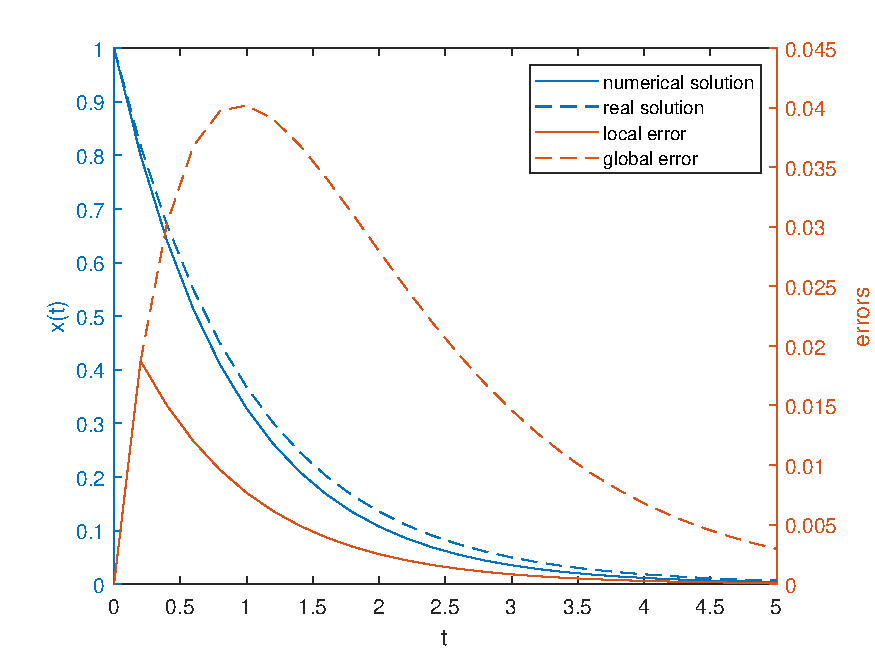
\includegraphics[width=\linewidth]{images/1/1_3_explicit_0_2.pdf} 
        \caption{Explicit Euler}
    \end{subfigure}%\hfill
    \begin{subfigure}{0.5\linewidth}
        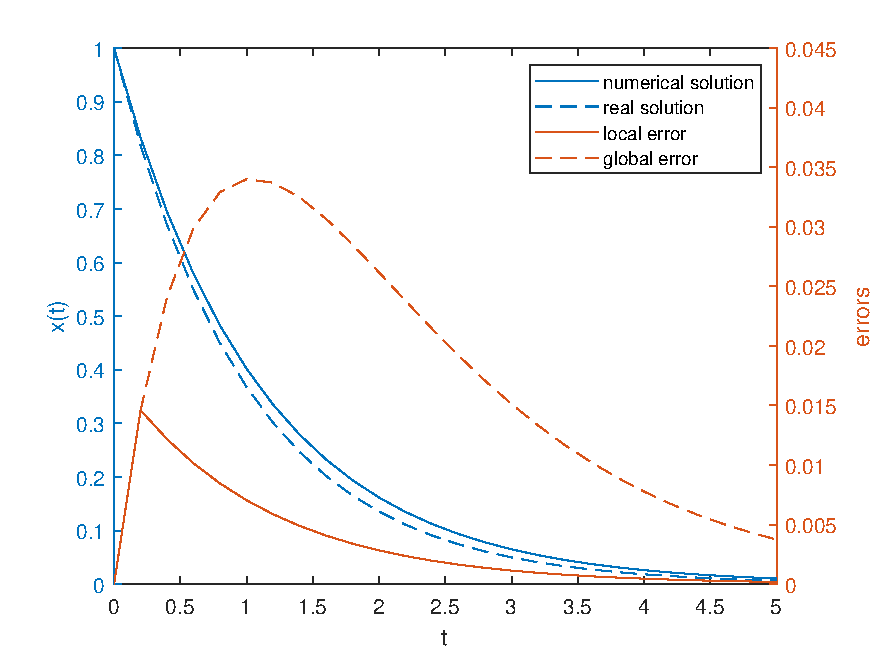
\includegraphics[width=\linewidth]{images/1/1_3_implicit_0_2.pdf}
        \caption{Implicit Euler}
    \end{subfigure}
    \caption{Local and global errors of the test equation}
    \label{1_3_errors}
\end{figure}

In these plots we can observe the two methods in action, and how they lend us a different result. For this particular time step size both the local and global error in the implicit Euler are lower than in the explicit one.

%%%%%%%%%%%%%%%%%%%%%%%%%%%%%%%%%%%%%%%%%%%%%%%%%%%%%%%%%%%%%%%%%%%%%%%%%%%%%%%%%%%%%%%%%%%%%%%%%%%

\subsection{Plot the local error vs the time step for the explicit Euler method and
the implicit Euler method. Does the plot behave as you would expect.
Explain what we mean by order. What is the order of the explicit Euler
method and the implicit Euler method, respectively. You should base your
answer on your numerical simulations. Is this as you would expect using
asymptotic theoretical considerations?} \label{1_4}

In Ascher-Petzold chapter 3.2 \cite{Ascher-Petzold} we find a definition of consistency of the method. We can find the order of consistency of these methods through the \textit{local truncation error}. In the book there's a derivation for the explicit Euler method that yields:
\begin{equation*}
    \mathbf{d}_n = \frac{h_n}{2}\mathbf{y}''(t_{n-1}) + \mathcal{O}(h_n^2).
\end{equation*}
Therefore, we can conclude the explicit Euler method is consistent of order 1. Using Dahlquist theorem \cite{Dahlquist_1956}, as the method is also zero-stable we know the method is convergent of order 1. Later in the chapter, the local error (here written as $\mathbf{l}_n$) is defined. Equation (3.14) in \cite{Ascher-Petzold} reads:
\begin{equation*}
    h_n|\mathcal{N}_h \hat{\mathbf{y}}(t_n)| = |\mathbf{l}_n|(1 + \mathcal{O}(h_n)).
\end{equation*}
We can therefore conclude that the local error will have order $1+1=2$.

We can follow a similar reasoning for obtaining the orders of the implicit Euler. We define the difference operator of the implicit Euler as:
\begin{equation*}
    \mathcal{N}_h u(t_n) = \frac{u(t_n) - u(t_{n-1})}{h_n} - f(t_n, u(t_n)).
\end{equation*}

Using Taylor's expansion $y(t_{n-1}) = y(t_n) - h_n y'(t_n) + \frac{h_n^2}{2}y''(t_n) + \ldots$ we get a local truncation error:
\begin{align*}
    \mathbf{d}_n &= \mathcal{N}_h y(t_n) = \frac{y(t_n) - y(t_{n-1})}{h_n} - f(t_n, y(t_n)) \\
    &= \frac{y(t_n) - \left[ y(t_n) - h_n y'(t_n) + \frac{h_n^2}{2}y''(t_n) + \mathcal{O}(h_n^3) \right]}{h_n} - y'(t_n) \\
    &= - \frac{h_n}{2}\mathbf{y}''(t_n) + \mathcal{O}(h_n^2).
\end{align*}
Therefore, we can conclude that the Implicit Euler is consistent of order 1. Notice that we get a different sign as in the explicit Euler, and this is completely consistent with what we see in figure \ref{1_3_errors}. As the implicit Euler is also zero-stable we know that the method is also convergent of order 1. Just as before, the local error should also scale with order 2 with the time step size.

Computing the mean of the local and the global error for the test equation with $\lambda=-1$, $x_0 = 1$, $\code{tspan}=[0, 20]$ and different time step sizes, ranging from $h=0.01$ to $0.5$ we finally obtain the results shown in Figure \ref{1_4_5_errors}. The local error escalates as a function of $h^2$ for both methods, just as what was expected from the mathematical derivation. 

\begin{figure}[h!]
\centering
    \begin{subfigure}{0.5\linewidth}
        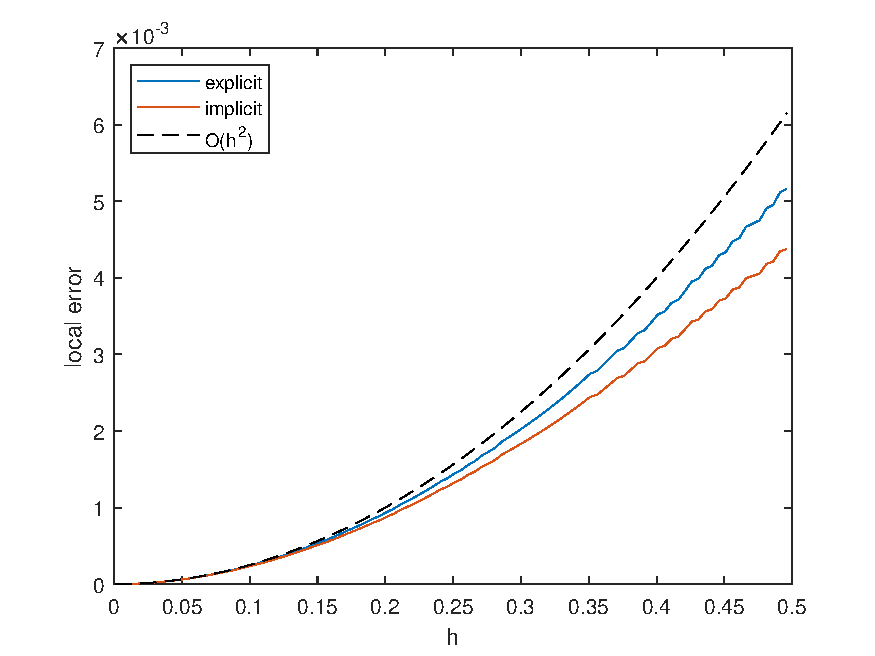
\includegraphics[width=\linewidth]{images/1/1_4_localerror.pdf} 
        \caption{Local Error}
    \end{subfigure}%\hfill
    \begin{subfigure}{0.5\linewidth}
        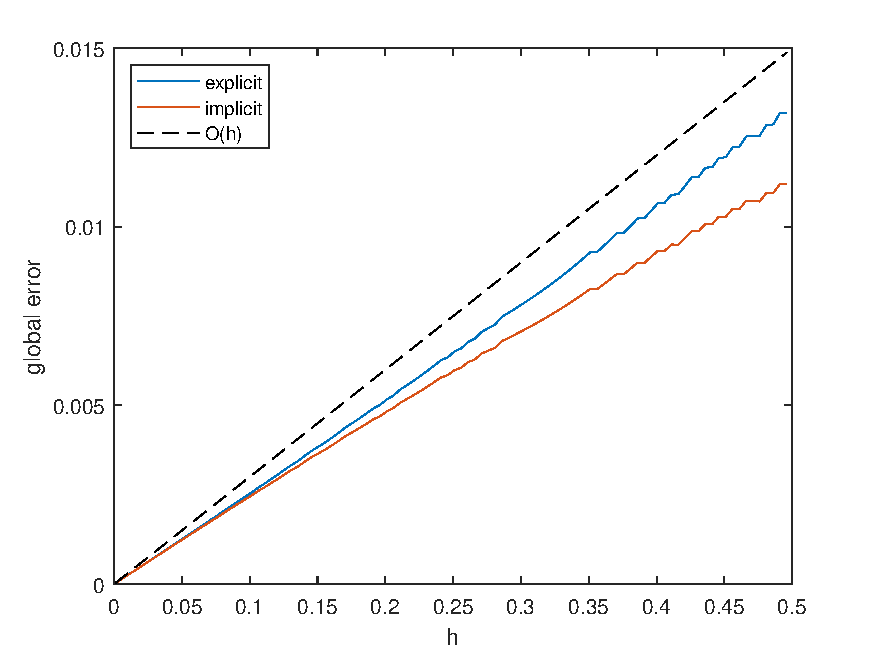
\includegraphics[width=\linewidth]{images/1/1_5_globalerror.pdf}
        \caption{Global Error}
    \end{subfigure}
    \caption{Errors of the Test Equation}
    \label{1_4_5_errors}
\end{figure}

%%%%%%%%%%%%%%%%%%%%%%%%%%%%%%%%%%%%%%%%%%%%%%%%%%%%%%%%%%%%%%%%%%%%%%%%%%%%%%%%%%%%%%%%%%%%%%%%%%%

\subsection{Plot the global error vs the time step for the explicit Euler method and
the implicit Euler method. Does the plot behave as you would expect.}
Following what we got in the previous exercise, as both methods have order 1 the global error should scale linearly with $h$. Taking a look at Figure \ref{1_4_5_errors}, we can see that the global error behaves as expected for both methods. It's also worth mentioning that the Implicit method has a lower local and global error for the test equation. This makes total sense if we analyze the expression of the local truncation error obtained in the previous exercise.

%%%%%%%%%%%%%%%%%%%%%%%%%%%%%%%%%%%%%%%%%%%%%%%%%%%%%%%%%%%%%%%%%%%%%%%%%%%%%%%%%%%%%%%%%%%%%%%%%%%

\subsection{Explain stability of a method and derive the expressions for the stability of
the explicit Euler method and the implicit Euler method. Plot the stability
regions. Explain A-stability. Is the explicit Euler-method A-stable? Is the
implicit Euler method A-stable?}

The concept of stability of a method comes from the concept of stability of a given problem. When looking at the Test Equation system in \ref{test_equation} (with $\lambda \in \mathbb{C}$), we can distinguish three different cases:
\begin{itemize}
    \item $\text{Re}(\lambda) > 0$, the solution grows exponentially with $t$ and the problem is \textit{unstable}. The distance between solution curves increases in time. In linear problems, the space of the solution (in this case $\mathbb{R}$) is then referred as the \textit{unstable space}
    \item $\text{Re}(\lambda) = 0$, the solution is either oscillating or 0, making the distance between solution curves to stay constant over time. This is referred as the \textit{center space}
    \item $\text{Re}(\lambda) < 0$, then the exponential decreases over time. The distance between curves decreases and the problem is \textit{asymptotically stable}. This yields an additional \textit{absolute stability} requirement:
    \begin{equation} \label{stability_requirement}
        |x_n| \leq |x_{n-1}|, \quad \forall n.
    \end{equation}
\end{itemize}

If we now take a look at how the Explicit Euler method is calculated iteratively for the Test Equation:
\begin{equation*}
    x_{n + 1} = x_n + h\lambda x_n = (1+h\lambda) x_n = (1+h\lambda)^2 x_{n-1} = \cdots = (1+h\lambda)^{n+1} x_0.
\end{equation*}
The only way \ref{stability_requirement} is going to be met is if:
\begin{equation*}
    |1+h\lambda| \leq 1.
\end{equation*}
This restricts the stability of the Explicit Euler to certain values of $h\lambda$. This region is depicted coloured in Figure \ref{stability_regions}.

For the Implicit Euler:
\begin{equation*}
     x_{n + 1} = x_n + h\lambda x_{n+1} = (1-h\lambda)^{-1} x_n = (1-h\lambda)^{-2} x_{n-1} = \cdots = (1-h\lambda)^{-(n+1)} x_0.
\end{equation*}
The stability condition in this case is:
\begin{equation*}
    \frac{1}{|1-h\lambda|} \leq 1.
\end{equation*}
This region is also depicted in Figure \ref{stability_regions}.

This leads us to the concept of A-Stability. A method is considered \textit{A-stable} if its region of absolute stability contains the entire left half-plane of $z=h\lambda$, i.e. $\text{Re}(h\lambda) < 0$. From Figure \ref{stability_regions} we can conclude that the Explicit Euler is not A-stable, while the Implicit Euler is.

\begin{figure}[h!]
\centering
    \begin{subfigure}{0.5\linewidth}
        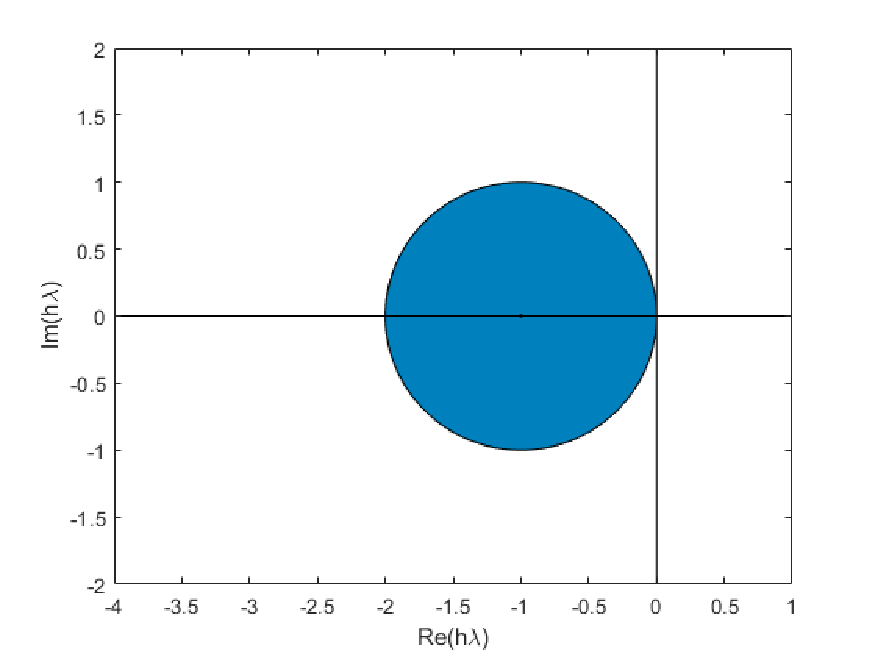
\includegraphics[width=\linewidth]{images/1/1_6_explicit.pdf} 
        \caption{Explicit Euler}
    \end{subfigure}%\hfill
    \begin{subfigure}{0.5\linewidth}
        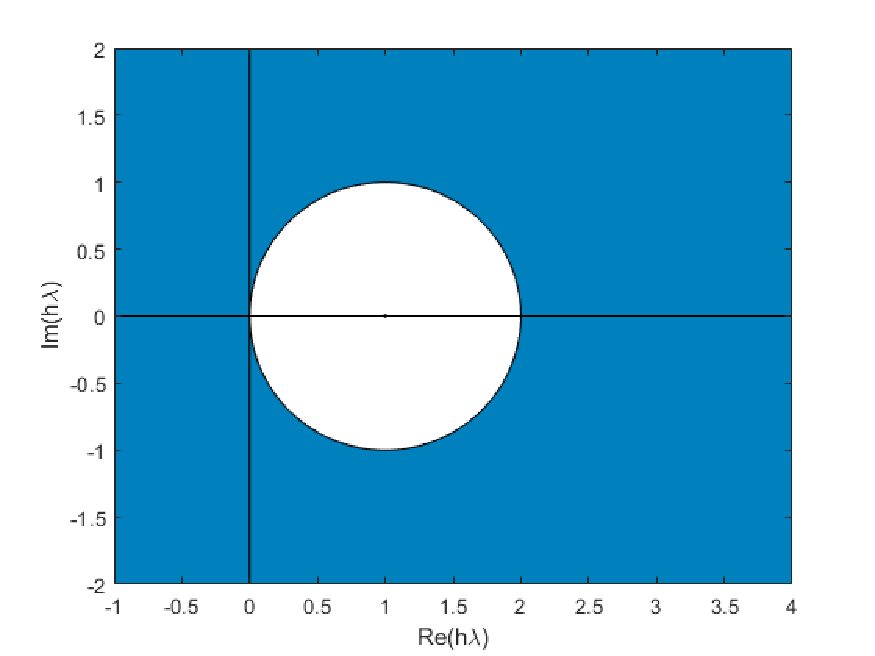
\includegraphics[width=\linewidth]{images/1/1_6_implicit.pdf}
        \caption{Implicit Euler}
    \end{subfigure}
    \caption{Absolute stability regions}
    \label{stability_regions}
\end{figure}
\pagebreak

\section{Explicit ODE solver} \label{part2}
We consider the initial value problem
\begin{equation} \label{2_problem}
    \Dot{x}(t) = f(t,x(t),p), \hspace{1em} x(t_0) = x_0,
\end{equation}
where $x \in \mathbb{R}^{n_x}$ and $p \in \mathbb{R}^{n_p}$.

\subsection{Describe the explicit Euler algorithm (i.e. provide an algorithm for it in your report and explain how you get from the differential equations to the numerical formulas).}

Taking a solution $x(t)$ of the IVP (\ref{2_problem}), we consider its Taylor expansion around time $t_0$:
\begin{align*}
    x(t_0 + h) &= x(t_0) + hx'(t_0) + \frac{h^2}{2}x''(t_0) + \mathcal{O}(h^3) \\
    & \approx x(t_0) + hx'(t_0).
\end{align*}
By ignoring quadratic terms and noticing that $x'(t) = f(t, x(t), p)$ we get the expression of the Explicit Euler method. If we discretize time as $t_n = t_0 + n \cdot h \, : 0 \leq n \leq N$ we can calculate a mesh function $x_n$ at each point in the following way:
\begin{align*}
    x_0 &= x(t_0), \\
    x_n &= x_{n-1}  + h f(t_{n-1}, x_{n-1}, p) \hspace{1em} \text{for } n = 1, 2, \ldots, N.
\end{align*}
The numerical solution $x_n \to x(t_n)$ as $h \to 0$. This is proven by the derivation of convergence and global error order of the method in exercise \ref{1_4}.

%%%%%%%%%%%%%%%%%%%%%%%%%%%%%%%%%%%%%%%%%%%%%%%%%%%%%%%%%%%%%%%%%%%%%%%%%%%%%%%%%%%%%%%%%%%%%%%%%%%

\subsection{Implement an algorithm in Matlab for the explicit Euler method with fixed time-step and provide this in your report. Use a format that enables syntax highlighting.}
\begin{lstlisting}[caption = Explicit Euler method with fixed time step size, captionpos=b, label=2_ExEuler_fixed]
function [T,X] = EulerExplicit_fixed(fun, tspan, h, x0, args)

t0 = tspan(1);
tf = tspan(end);
T = t0:h:tf;
N = size(T,2);
X = zeros(size(x0,1), N);
X(:,1) = x0;

for k = 1:N-1
    f = feval(fun, T(k), X(:,k), args{:});
    X(:,k+1) = X(:,k) + h * f;
end
end

\end{lstlisting}

%%%%%%%%%%%%%%%%%%%%%%%%%%%%%%%%%%%%%%%%%%%%%%%%%%%%%%%%%%%%%%%%%%%%%%%%%%%%%%%%%%%%%%%%%%%%%%%%%%%

\subsection{Implement an algorithm in Matlab for the explicit Euler method with adaptive time step and error estimation using step doubling.}
In this implementation we use an asymptotic time step controller. As we are going to model problems without an analytical solution, we'll use step doubling to make an estimate of the error.

\begin{lstlisting}[caption = Explicit Euler method with adaptive time step size, captionpos=b, label=2_ExEuler_adaptive]
function [T,X,r_out,h_out,info] = EulerExplicit_adaptive(fun,tspan,h0,x0,abstol,reltol,args)

epstol = 0.8;
facmin = 0.1;
facmax = 5.0;

t0 = tspan(1);
tf = tspan(end);
t = t0;
h = h0;
x = x0;

T = t0;
X = x0;
r_out = [];
h_out = [];
info = zeros(1,4);

nfun = 0;
nstep = 0;
naccept = 0;

while t < tf
    if (t+h > tf)
        h = tf-t;
    end
    f = feval(fun,t,x,args{:});
    nfun = nfun + 1;
    AcceptStep = false;
    while ~AcceptStep
        x1 = x + h*f;
        
        hm = 0.5*h;
        tm = t + hm;
        xm = x + hm*f;
        fm = feval(fun,tm,xm,args{:});
        nfun = nfun + 1;
        x1hat = xm + hm*fm;
        
        nstep = nstep + 1;
        
        e = abs(x1hat-x1);
        r = max(e./max(abstol, abs(x1hat) .* reltol));
        AcceptStep = (r <= 1.0);
        
        if AcceptStep
            t = t+h;
            x = x1hat;
            
            T = [T,t];
            X = [X,x];
            r_out = [r_out, r];
            h_out = [h_out, h];
            naccept = naccept + 1;
        end
        
        h = max(facmin, min(sqrt(epstol/r), facmax)) * h;
    end
end

info(1) = nfun;
info(2) = nstep;
info(3) = naccept;
info(4) = nstep - naccept;

end

\end{lstlisting}

% \pagebreak

%%%%%%%%%%%%%%%%%%%%%%%%%%%%%%%%%%%%%%%%%%%%%%%%%%%%%%%%%%%%%%%%%%%%%%%%%%%%%%%%%%%%%%%%%%%%%%%%%%%

\subsection{Test your algorithms on the Van der Pol problem \texorpdfstring{($\mathbf{\mu = 1.5}$ and $\mathbf{\mu = 15}$, $\mathbf{x_0 = [1.0;1.0]}$)}{mu = 1.5 and mu = 15, x0 = [1.0;1.0]}} \label{2_4}
The IVP (\ref{2_problem}) for the Van der Pol problem will be used in the entire assignment by calling the following function:

\begin{lstlisting}[caption = Van der Pol equation, captionpos=b, label=VDP_eq]
function xdot = VanderPol(t,x,mu)
xdot = zeros(2,1);
xdot(1) = x(2);
xdot(2) = mu*(1-x(1)^2)*x(2) - x(1);
end
\end{lstlisting}

Both methods will be called simply by setting the parameters and respectively:
\begin{lstlisting}
[T,X] = EulerExplicit_fixed(@VanderPol, tspan, h, x0, args);
[T,X,r_out,h_out,info] = EulerExplicit_adaptive(@VanderPol, tspan, h0, x0, abstol, reltol, args);
\end{lstlisting}

In the following plots we can observe the results of the Explicit Euler method with fixed and adaptive step size, both solving the Van der Pol problem for a $\mu$ of $1.5$ and $15$. The solutions are plotted using different step sizes for the fixed method and different tolerances for the adaptive method. The tolerance value sets both the values of \code{abstol} and \code{reltol}.

Taking a look at the results for the fixed method in Figures \ref{2_4_fixed_mu_1_5} and \ref{2_4_fixed_mu_15}, we can spot a curious behaviour. Even though the shape of the solution for high step sizes looks alike to the real solution, there is a considerable frequency difference among them. We can also see how for $\mu=15$ the problem becomes more \textit{stiff}, thus requiring a smaller step size (values of $h \sim 0.2$ made it explode).

The same behaviours can also be observed in the results for the adaptive method in Figures \ref{2_4_adaptive_mu_1_5} and \ref{2_4_adaptive_mu_15}. These plots also show the final chosen step size per every time iteration and the measure of the relative error. Of course, when the tolerance is very fine $h \to 0$ and $r \to 0.8$, which is the chosen value of \code{epstol}. For the case when $\mu = 15$, we can also observe the increase in stiffness in these two plots. Also, we can observe how the no. of function calls and steps varies when we decrease the tolerance value in Tables \ref{2_4_adaptive_mu_1_5_table} and \ref{2_4_adaptive_mu_15_table}.

\begin{figure}[H]
    \centering
    \makebox[\textwidth][c]{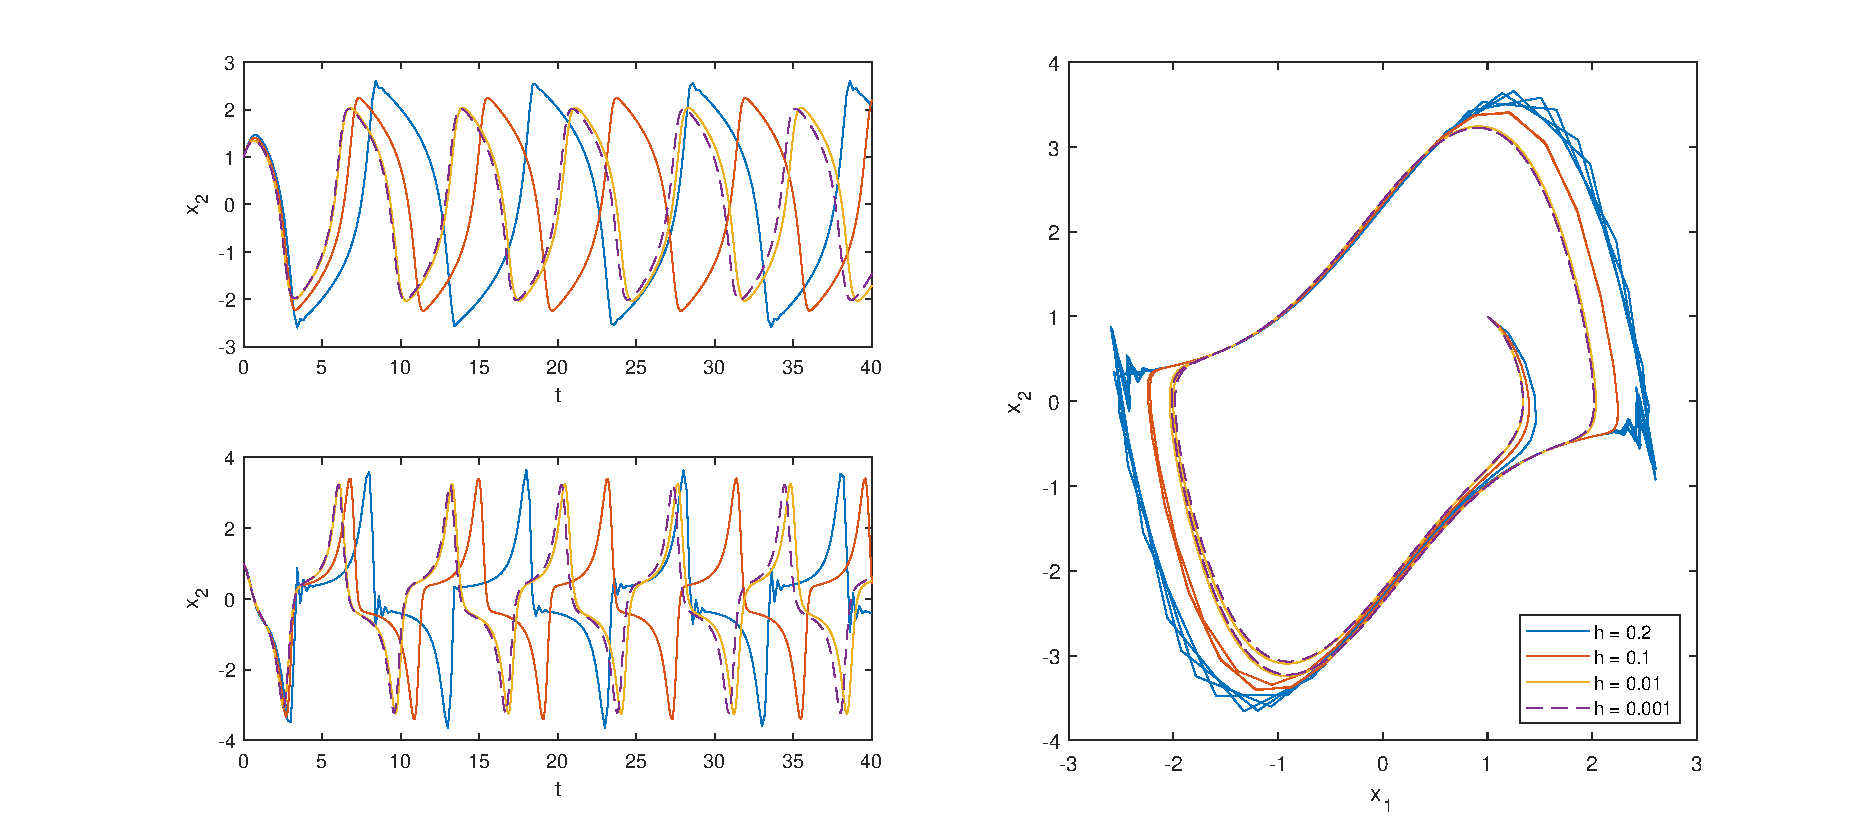
\includegraphics[width=1.25\textwidth]{images/2/2_4_fixed_mu_1_5.pdf}}
    \caption{Solution for the Van der Pol problem ($\mathit{\mu = 1.5}$) using Explicit Euler with fixed step size}
    \label{2_4_fixed_mu_1_5}
\end{figure}

\begin{figure}[H]
    \centering
    \makebox[\textwidth][c]{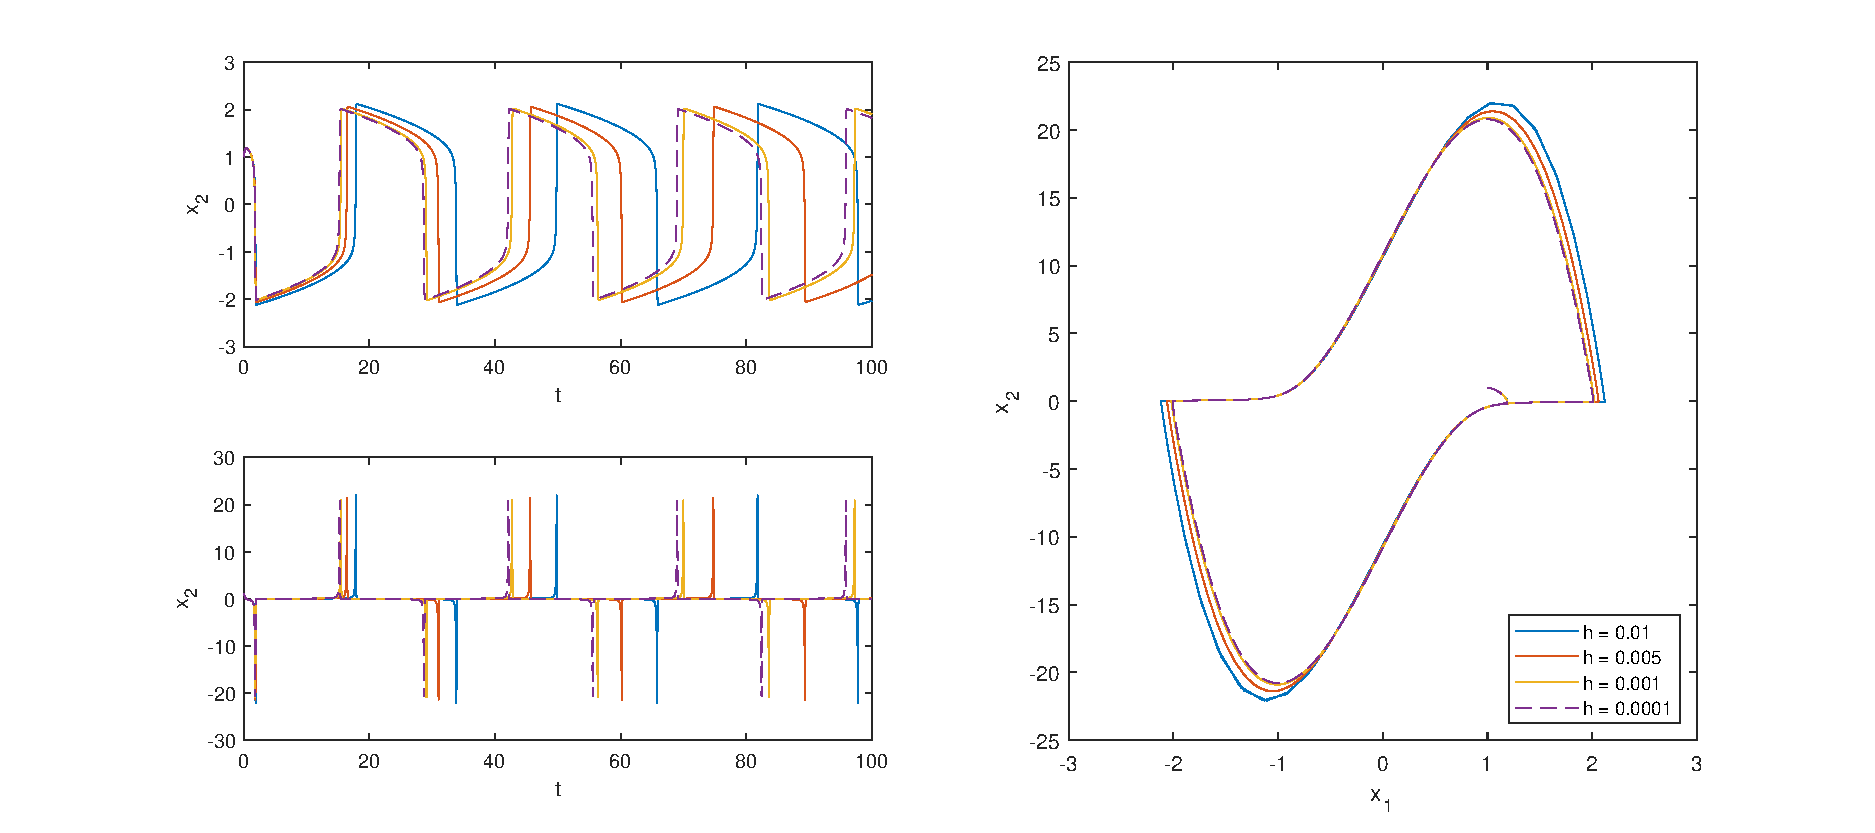
\includegraphics[width=1.25\textwidth]{images/2/2_4_fixed_mu_15.pdf}}
    \caption{Solution for the Van der Pol problem ($\mathit{\mu = 15}$) using Explicit Euler with fixed step size}
    \label{2_4_fixed_mu_15}
\end{figure}

\begin{figure}[H]
    \centering
    \makebox[\textwidth][c]{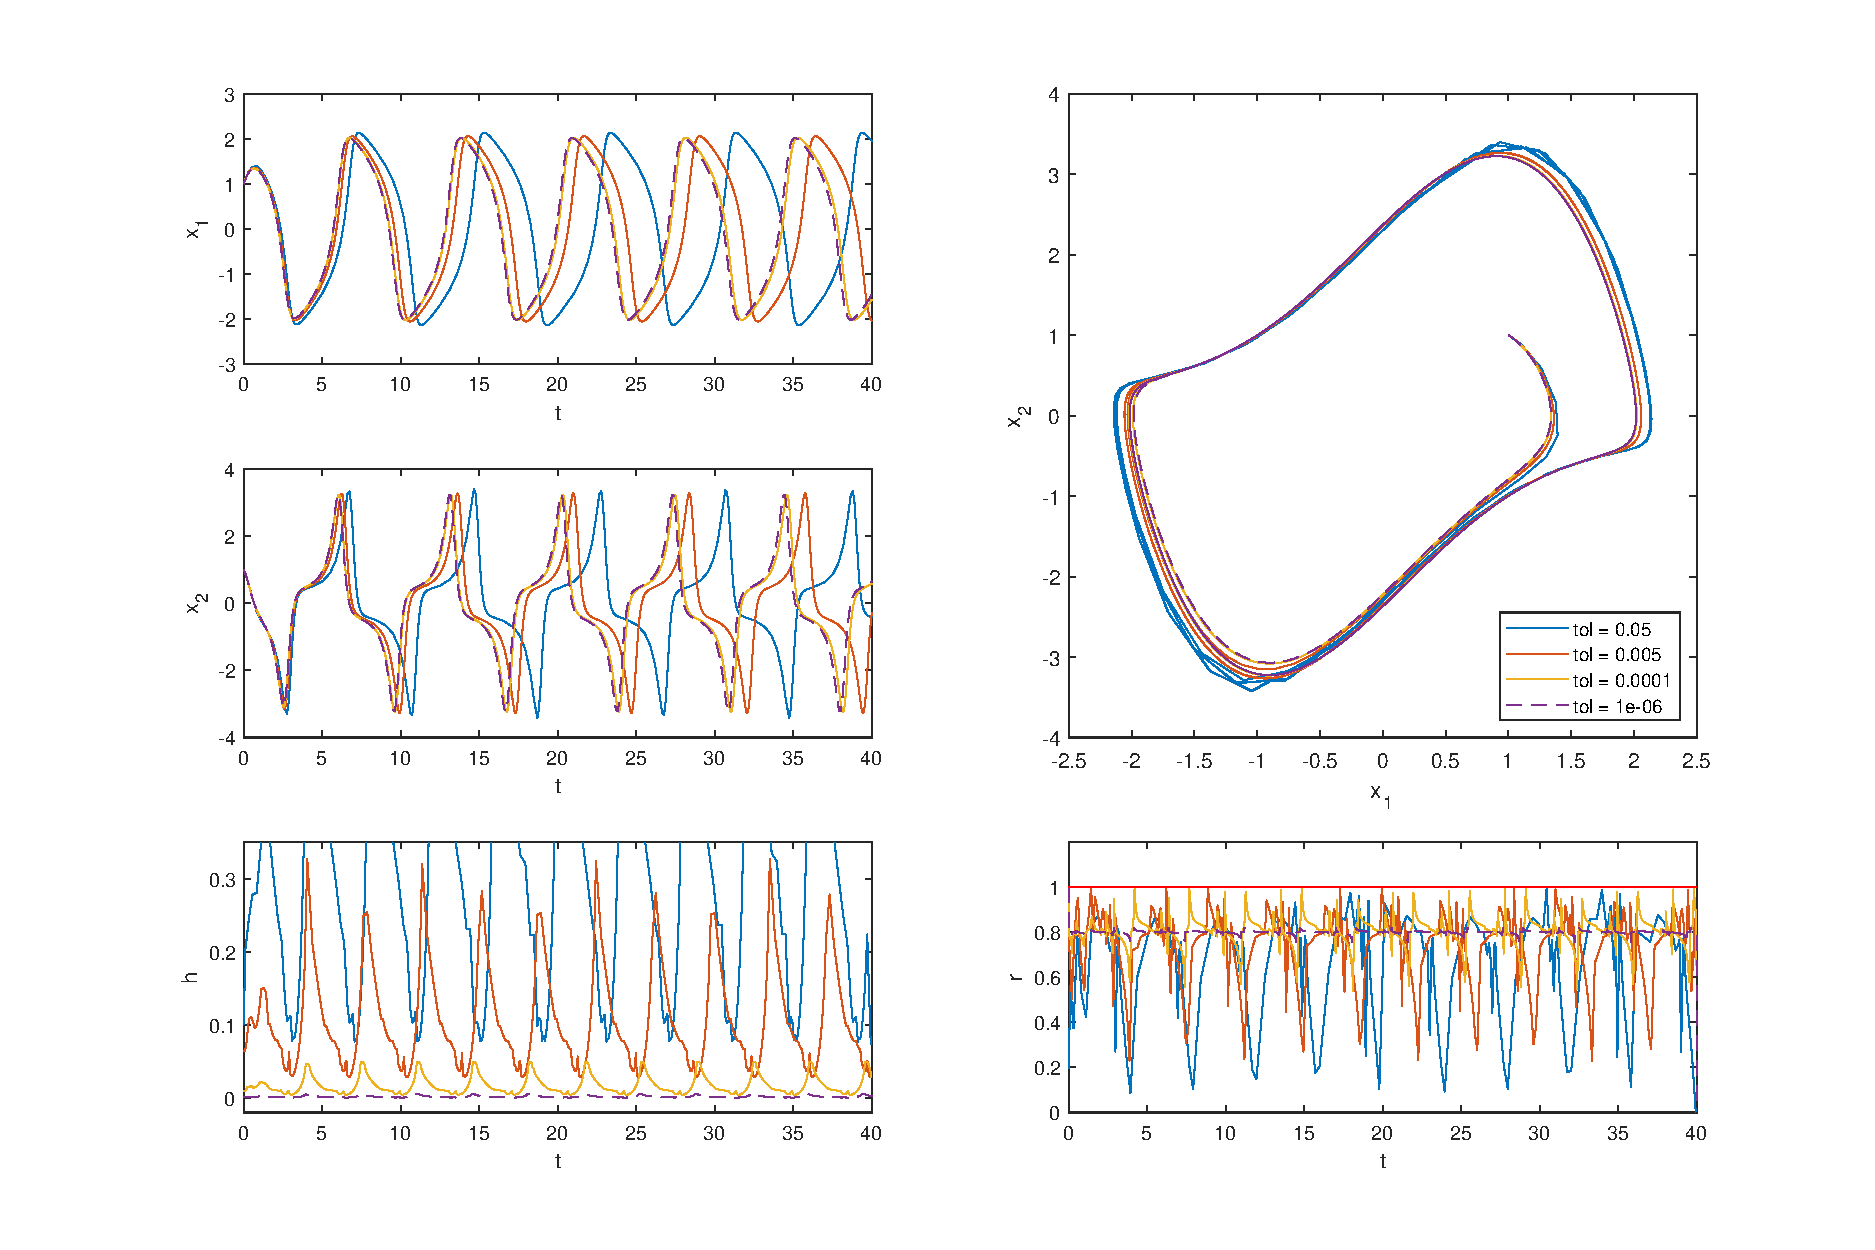
\includegraphics[width=1.25\textwidth]{images/2/2_4_adaptive_mu_1_5.pdf}}
    \caption{Solution for the Van der Pol problem ($\mathit{\mu = 1.5}$) using Explicit Euler with adaptive step size}
    \label{2_4_adaptive_mu_1_5}
\end{figure}

\begin{table}[H]
    \centering
    \begin{tabular}{@{}l|cccc@{}}
    \toprule
    Tolerances           & 0.05 & 0.005 & 0.0001 & 1e-06 \\ \midrule
    Function evaluations & 445  & 1200  & 7383   & 73678 \\
    Calculated steps     & 263  & 660   & 3695   & 36840 \\
    Accepted steps       & 182  & 540   & 3688   & 36838 \\
    Rejected steps       & 81   & 120   & 7      & 2     \\ \bottomrule
    \end{tabular}
    \caption{Parameters of the Explicit Euler with adaptive step size for the Van der Pol problem ($\mathit{\mu = 1.5}$)}
    \label{2_4_adaptive_mu_1_5_table}
\end{table}

\begin{figure}[H]
    \centering
    \makebox[\textwidth][c]{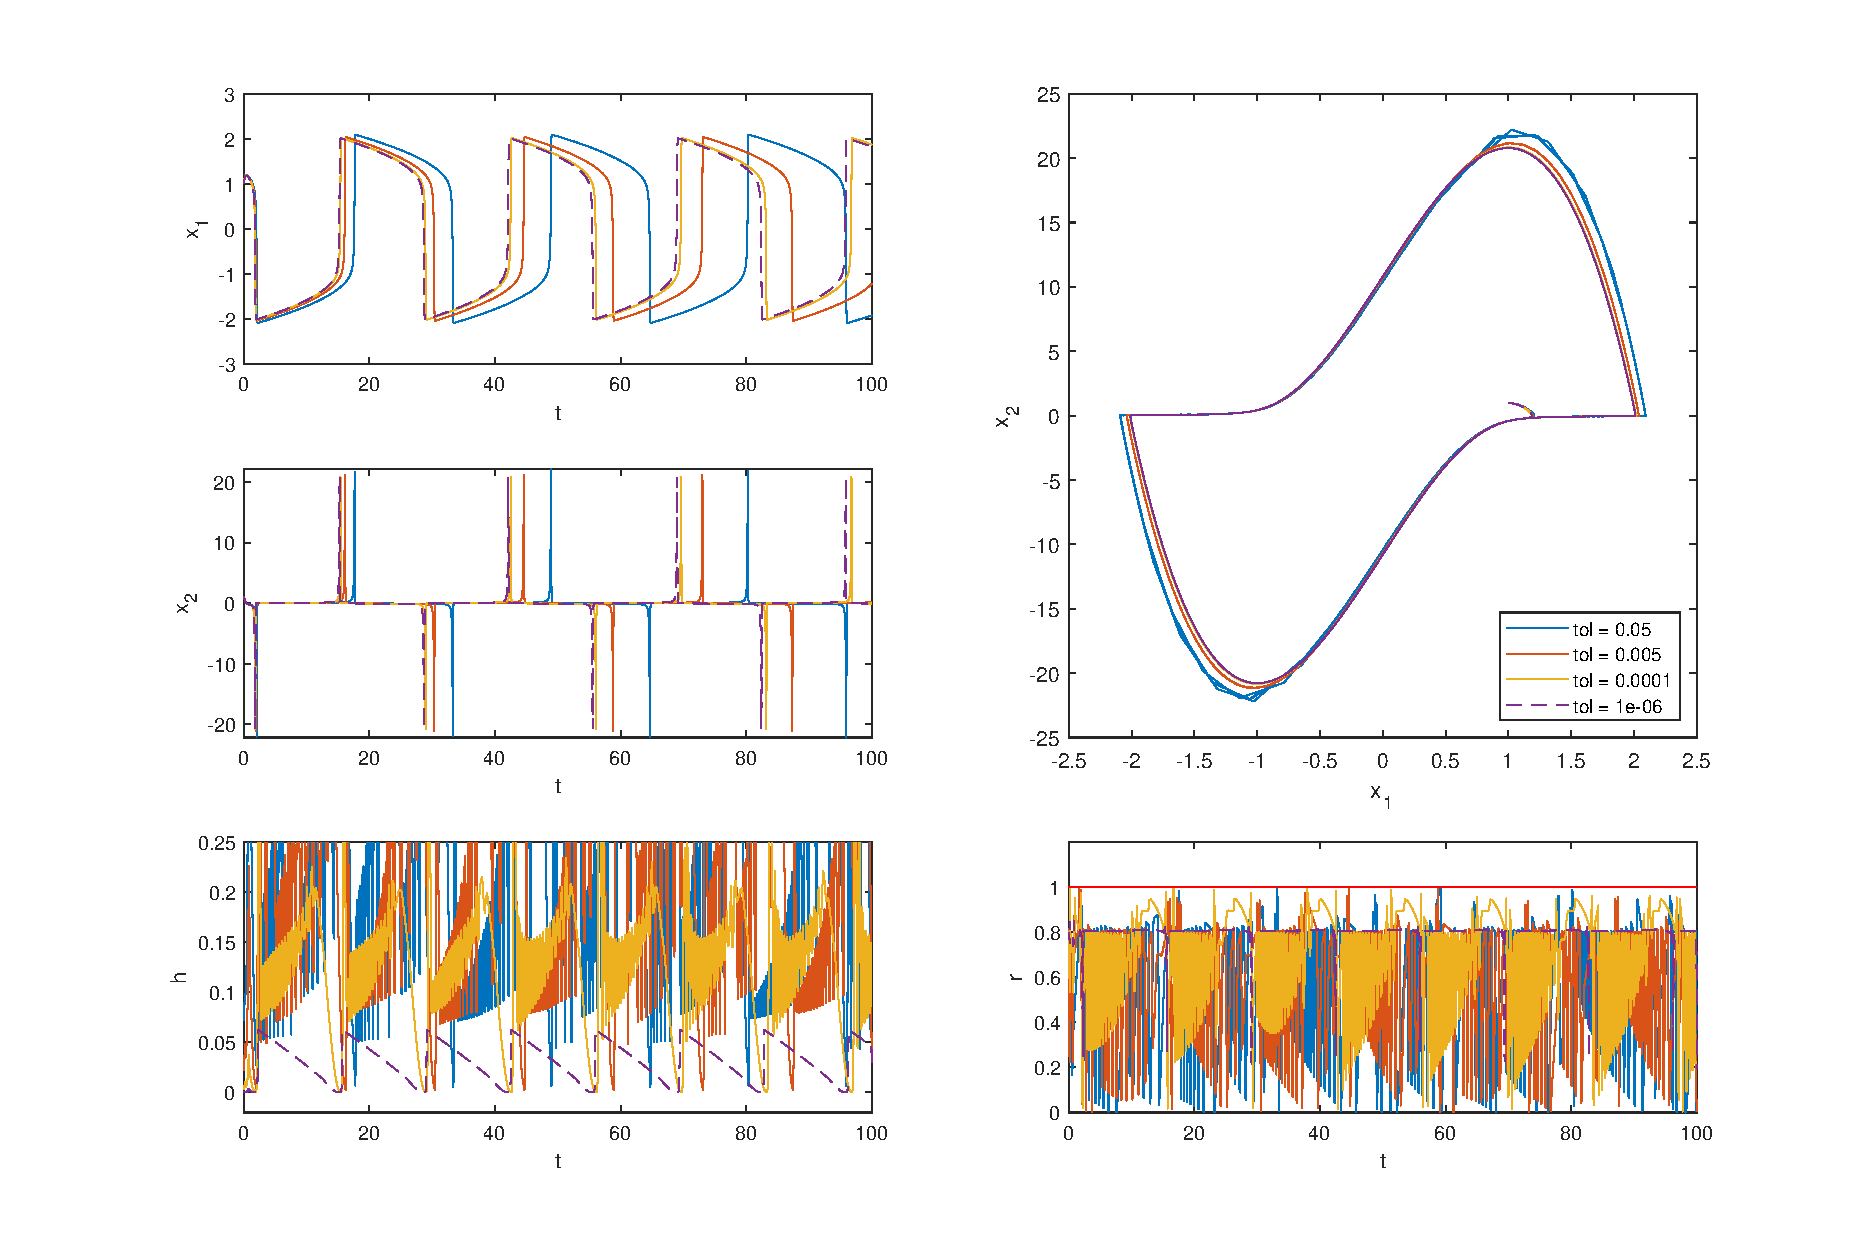
\includegraphics[width=1.25\textwidth]{images/2/2_4_adaptive_mu_15.pdf}}
    \caption{Solution for the Van der Pol problem ($\mathit{\mu = 15}$) using Explicit Euler with adaptive step size}
    \label{2_4_adaptive_mu_15}
\end{figure}

\begin{table}[H]
    \centering
    \begin{tabular}{@{}l|cccc@{}}    \toprule
    Tolerances           & 0.05 & 0.005 & 0.0001 & 1e-06      \\ \midrule
    Function evaluations & 1583 & 2485  & 11246  & 1.0404e+05 \\
    Calculated steps     & 954  & 1418  & 5740   & 52022      \\
    Accepted steps       & 629  & 1067  & 5506   & 52019      \\
    Rejected steps       & 325  & 351   & 234    & 3          \\ \bottomrule
    \end{tabular}
    \caption{Parameters of the Explicit Euler with adaptive step size for the Van der Pol problem ($\mathit{\mu = 15}$)}
    \label{2_4_adaptive_mu_15_table}
\end{table}

\pagebreak
\pagebreak
\pagebreak
\pagebreak
%%%%%%%%%%%%%%%%%%%%%%%%%%%%%%%%%%%%%%%%%%%%%%%%%%%%%%%%%%%%%%%%%%%%%%%%%%%%%%%%%%%%%%%%%%%%%%%%%%%

\subsection{Test your algorithms on the adiabatic CSTR problem described in the papers uploaded to Learn (3D-version and 1D-version).}
The IVPs (\ref{2_problem}) for both versions of the CSTR problem, obtained from \cite{Bagterp1} and \cite{Bagterp2} are included in the following functions:

\begin{lstlisting}[caption = CSTR 3D equation, captionpos=b, label=CSTR_3D_eq]
function xdot = CSTR_3D(t,x,F,params)
% F to IS units
F = F/60000;

beta = params(1);
k0 = params(2);
EaR = params(3);
CAin = params(4);
CBin = params(5);
Tin = params(6);
V = params(7);

CA = x(1);
CB = x(2);
T = x(3);
xdot = zeros(3,1);

% Rate of reaction
r = k0 * exp(-EaR/T) * CA * CB;
% Production rates and rate of temperature
RA = -r;
RB = -2*r;
RT = beta*r;
% Final ODE
xdot(1) = F/V * (CAin - CA) + RA;
xdot(2) = F/V * (CBin - CB) + RB;
xdot(3) = F/V * (Tin - T) + RT;
end

\end{lstlisting}

\begin{lstlisting}[caption = CSTR 1D equation, captionpos=b, label=CSTR_1D_eq]
function Tdot = CSTR_1D(t, T, F, params)
% F to IS units
F = F/60000;

beta = params(1);
k0 = params(2);
EaR = params(3);
CAin = params(4);
CBin = params(5);
Tin = params(6);
V = params(7);

% Rate of reaction
r = k0 * exp(-EaR/T) * (CAin + 1/beta * (Tin - T)) * (CBin + 2/beta * (Tin - T));
% Rate of temperature
RT = beta * r;
% Final ODE
Tdot = F/V*(Tin - T) + RT;
end

\end{lstlisting}

Just as in \cite{Bagterp1} and \cite{Bagterp2}, the flow will be a function of time. Its shape can be seen in Figure \ref{2_5_3D_trial}, together with a solution for the 3D-CSTR problem. The way to call the method having this flow function over time is slightly trickier than in the Van der Pol problem. I tried first creating F as a piecewise function and substituting the time in every CSTR function call. However, this was proven to be very time consuming as it implied working with symbolic functions. The best way of achieving the same output was by:
\pagebreak
\begin{lstlisting}
% Piecewise flow definition
tspans = [[0,3];[3,5];[5,7];[7,9];[9,12];[12,16];[16,18];...
    [18,20];[20,22];[22,24];[24,28];[28,32];[32,35]];
Fs = [700,600,500,400,300,200,300,400,500,600,700,200,700];

T = [];
X = [];

for i=1:size(Fs,2)
    tspan = tspans(i,:)*60;
    F = Fs(i);
    args = {F, [beta,k0,EaR,CAin,CBin,Tin,V]};
    [T_local,X_local] = EulerExplicit_fixed(@CSTR_3D, tspan, h, x0, args);
    
    T = [T, T_local(1:end-1)];
    X = [X, X_local(:,1:end-1)];
    
    x0 = X_local(:,end);
end
% Add last point and normalize
T = [T,T_local(end)]/60;
X = [X, X_local(:,end)]-273;
\end{lstlisting}

\begin{figure}[H]
    \centering
    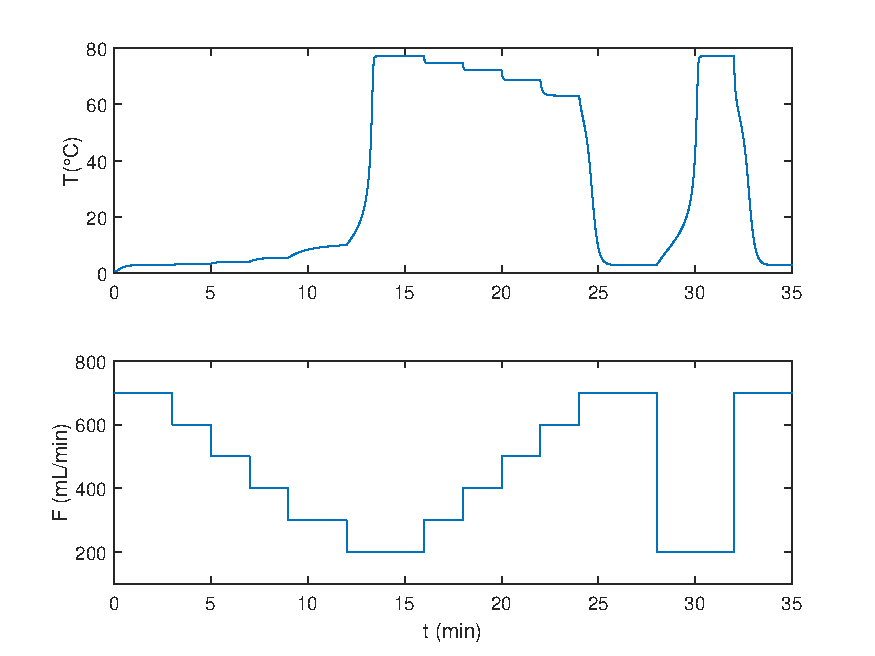
\includegraphics[width=0.8\textwidth]{images/2/2_5_3D_trial.pdf}
    \caption{Solution and value of the flow over time for the CSTR 3D problem}
    \label{2_5_3D_trial}
\end{figure}

The results for the 3D problem and 1D problem are very similar. This can be seen in Figure \ref{2_5_3D_vs_1D}, where a closeup of the interval $t \in [0,1.5]$ minutes is shown. This was the region where we can find the greatest difference between the two problems. The following plots show the results of different runs of the CSTR problems, for the fixed and adaptive Explicit Euler with different values of steps and tolerances respectively.

Taking a look at the results using the fixed method (Figure \ref{2_5_3D_1D_hs}), it's very difficult to spot a difference between the 3D and 1D case. The plot behaves the same for every chosen time step. However, the results from the adaptive in Figures \ref{2_5_3D_tols} and \ref{2_5_1D_tols} and Tables \ref{2_5_3D_tols_table} and \ref{2_5_1D_tols} are much more enlightening. In the 3D problem, the solution is pretty close even for the biggest tolerance of $0.05$. Moreover, we can observe some spike behaviour in the value of $r$ that coincides with every step change of the flow function. Also the problem becomes more stiff when the value of $F$ goes down (the r value and therefore change in h shifts a lot in these regions). This also explains the spike behaviour observed in the fixed method only at these points in time. Finally, we can observe that it takes a tighter tolerance for the 1D problem to converge. However, the number of function evaluations is a lot smaller than the 3D problem for the same tolerances and lowering down enough the tolerance yields pretty good results.

\begin{figure}[H]
    \centering
    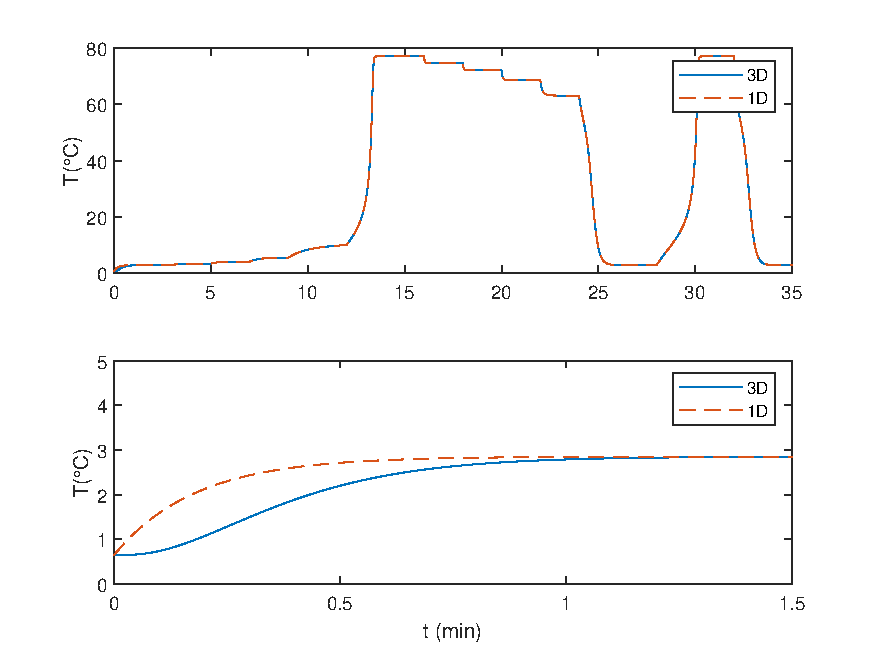
\includegraphics[width=0.8\textwidth]{images/2/2_5_3D_vs_1D.pdf}
    \caption{Comparison of the solutions for the CSTR 3D and 1D}
    \label{2_5_3D_vs_1D}
\end{figure}

\begin{figure}[H]
\centering
    \begin{subfigure}{0.8\linewidth}
        \centering
        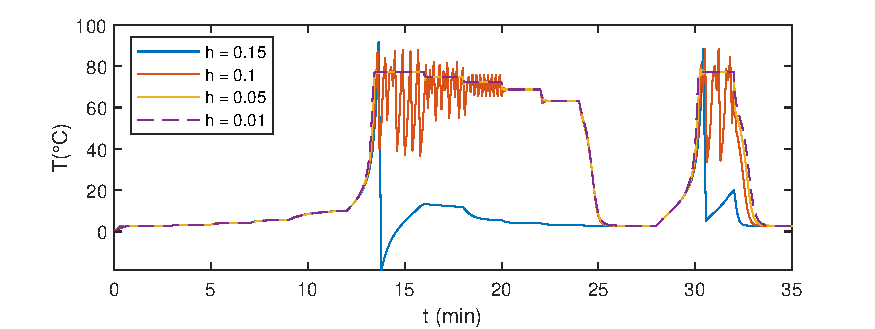
\includegraphics[width=1\linewidth]{images/2/2_5_3D_hs.pdf} 
        \caption{CSTR 3D problem}
    \end{subfigure} \\
    \begin{subfigure}{0.8\linewidth}
        \centering
        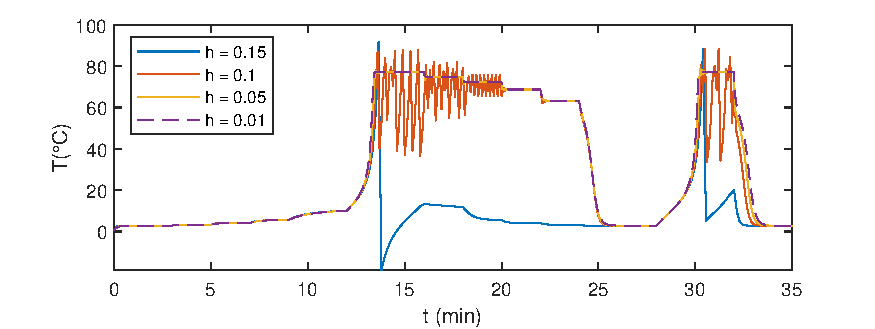
\includegraphics[width=1\linewidth]{images/2/2_5_1D_hs.pdf}
        \caption{CSTR 1D problem}
    \end{subfigure}
    \caption{Solution for the CSTR problem using Explicit Euler with fixed step size}
    \label{2_5_3D_1D_hs}
\end{figure}

\begin{figure}[H]
    \centering
    \makebox[\textwidth][c]{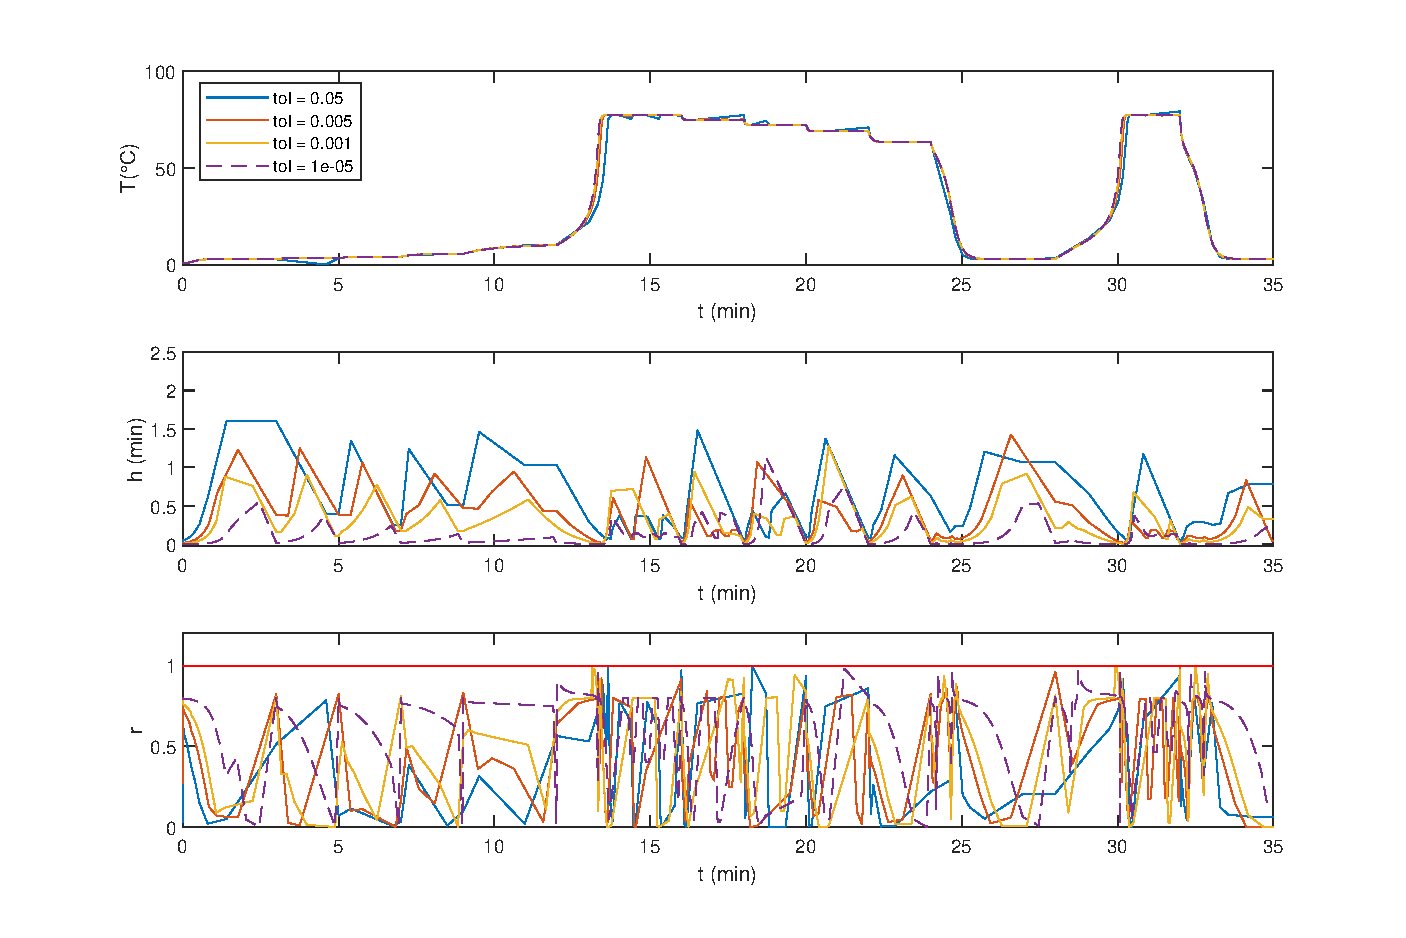
\includegraphics[width=1\textwidth]{images/2/2_5_3D_tols.pdf}}
    \caption{Solution for the CSTR 3D problem using Explicit Euler with adaptive step size}
    \label{2_5_3D_tols}
\end{figure}

\begin{table}[H]
    \centering
    \begin{tabular}{@{}l|cccc@{}}
    \toprule
    Tolerances           & 0.05 & 0.005 & 0.001 & 1e-05 \\ \midrule
    Function evaluations & 207  & 431   & 726   & 5250  \\
    Calculated steps     & 120  & 245   & 400   & 2657  \\
    Accepted steps       & 87   & 186   & 326   & 2593  \\
    Rejected steps       & 33   & 59    & 74    & 64    \\ \bottomrule
    \end{tabular}
    \caption{Parameters of the Explicit Euler with adaptive step size for the CSTR 3D problem}
    \label{2_5_3D_tols_table}
\end{table}

\begin{figure}[H]
    \centering
    \makebox[\textwidth][c]{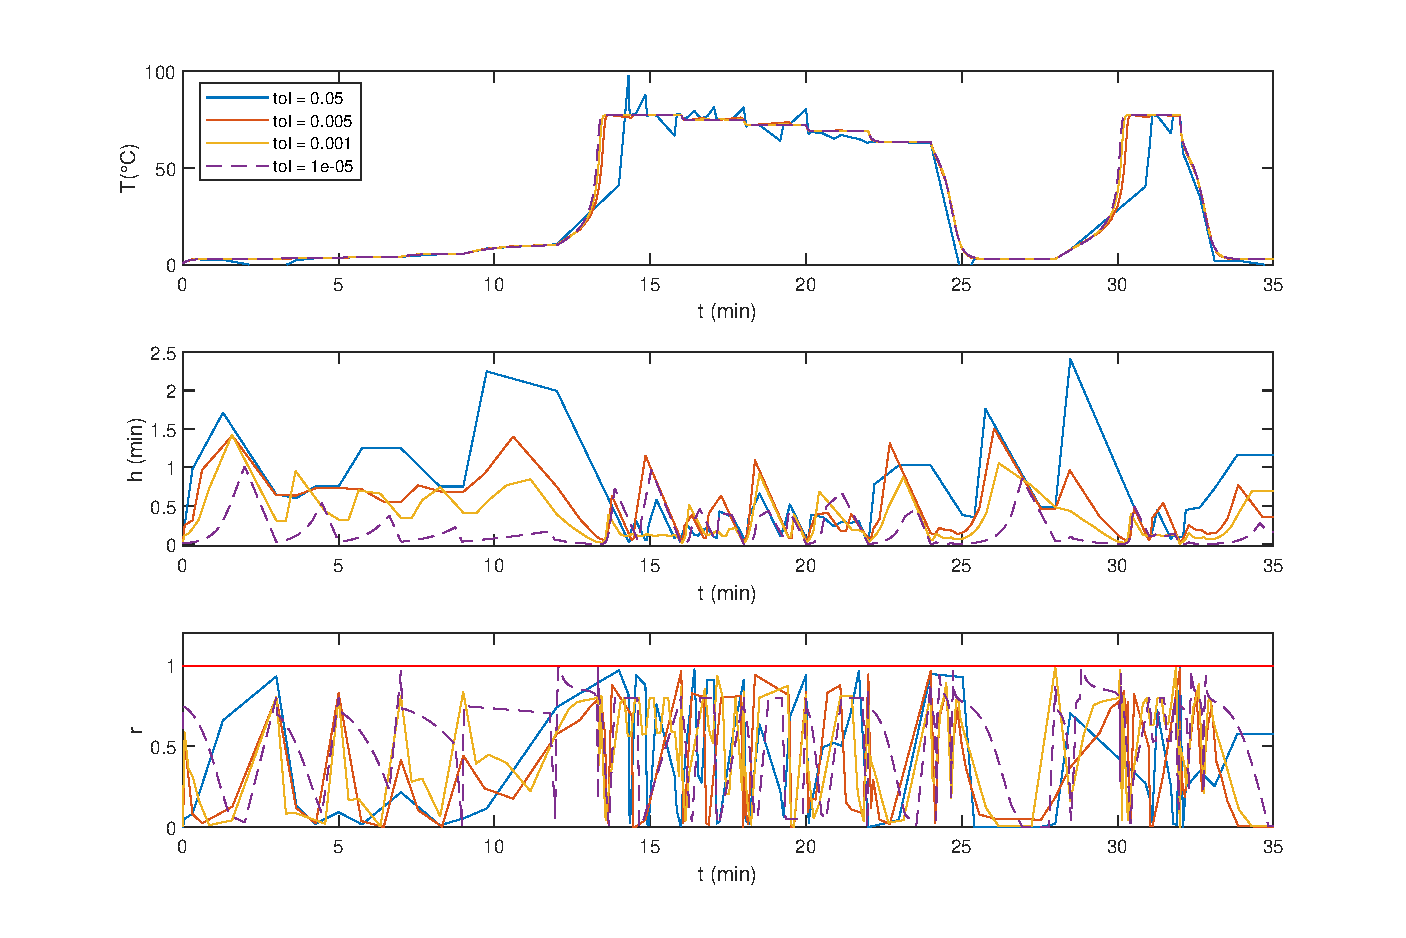
\includegraphics[width=1\textwidth]{images/2/2_5_1D_tols.pdf}}
    \caption{Solution for the CSTR 1D problem using Explicit Euler with adaptive step size}
    \label{2_5_1D_tols}
\end{figure}

\begin{table}[H]
    \centering
    \begin{tabular}{@{}l|cccc@{}}
    \toprule
    Tolerances           & 0.05 & 0.005 & 0.001 & 1e-05 \\ \midrule
    Function evaluations & 194  & 256   & 455   & 2285  \\
    Calculated steps     & 115  & 148   & 261   & 1171  \\
    Accepted steps       & 79   & 108   & 194   & 1114  \\
    Rejected steps       & 36   & 40    & 67    & 57    \\ \bottomrule
    \end{tabular}
    \caption{Parameters of the Explicit Euler with adaptive step size for the CSTR 1D problem}
    \label{2_5_1D_tols_table}
\end{table}

%%%%%%%%%%%%%%%%%%%%%%%%%%%%%%%%%%%%%%%%%%%%%%%%%%%%%%%%%%%%%%%%%%%%%%%%%%%%%%%%%%%%%%%%%%%%%%%%%%%
\pagebreak

\subsection{Compare the results from your algorithms with the results you get using some of Matlab's ODE solvers}
We'll compare the solution obtained with the explicit Euler to two ODE solvers from Matlab: \code{ode45} and \code{ode15s}. The first one is an implementation of the Dormand-Prince 5(4), a method from the Explicit Runge-Kutta family. Being an explicit method, it's not very good when dealing with stiff problems. \code{ode15s}, on the other hand, is designed to work specifically with these types of problems. Both of them are also of adaptive step size. For that reason, we will compare the Explicit Euler with adaptive step size to these two: see how they behave for a given tolerance and problem and analyse their increase in the number of function evaluations when narrowing down the tolerance.

For the Van der Pol problem, we tested Explicit Euler against \code{ode45} for the non-stiff case ($\mu = 1.5$), and against \code{ode15s} for the stiff case ($\mu = 15$). The obtained results for the Van der Pol problem (Figures \ref{2_6_mu_1_5} and \ref{2_6_mu_15} and Tables \ref{2_6_adaptive_mu_1_5_table} and \ref{2_6_adaptive_mu_15_table}) show what we discussed previously. The Explicit Euler works fine in the non-stiff case, even though the \code{ode45} achieves better accuracy with a fewer no. of function evaluations. In the stiff case, however, the no. of evaluations is ridiculously high compared to the \code{ode15s}.

\begin{figure}[H]
    \centering
    \makebox[\textwidth][c]{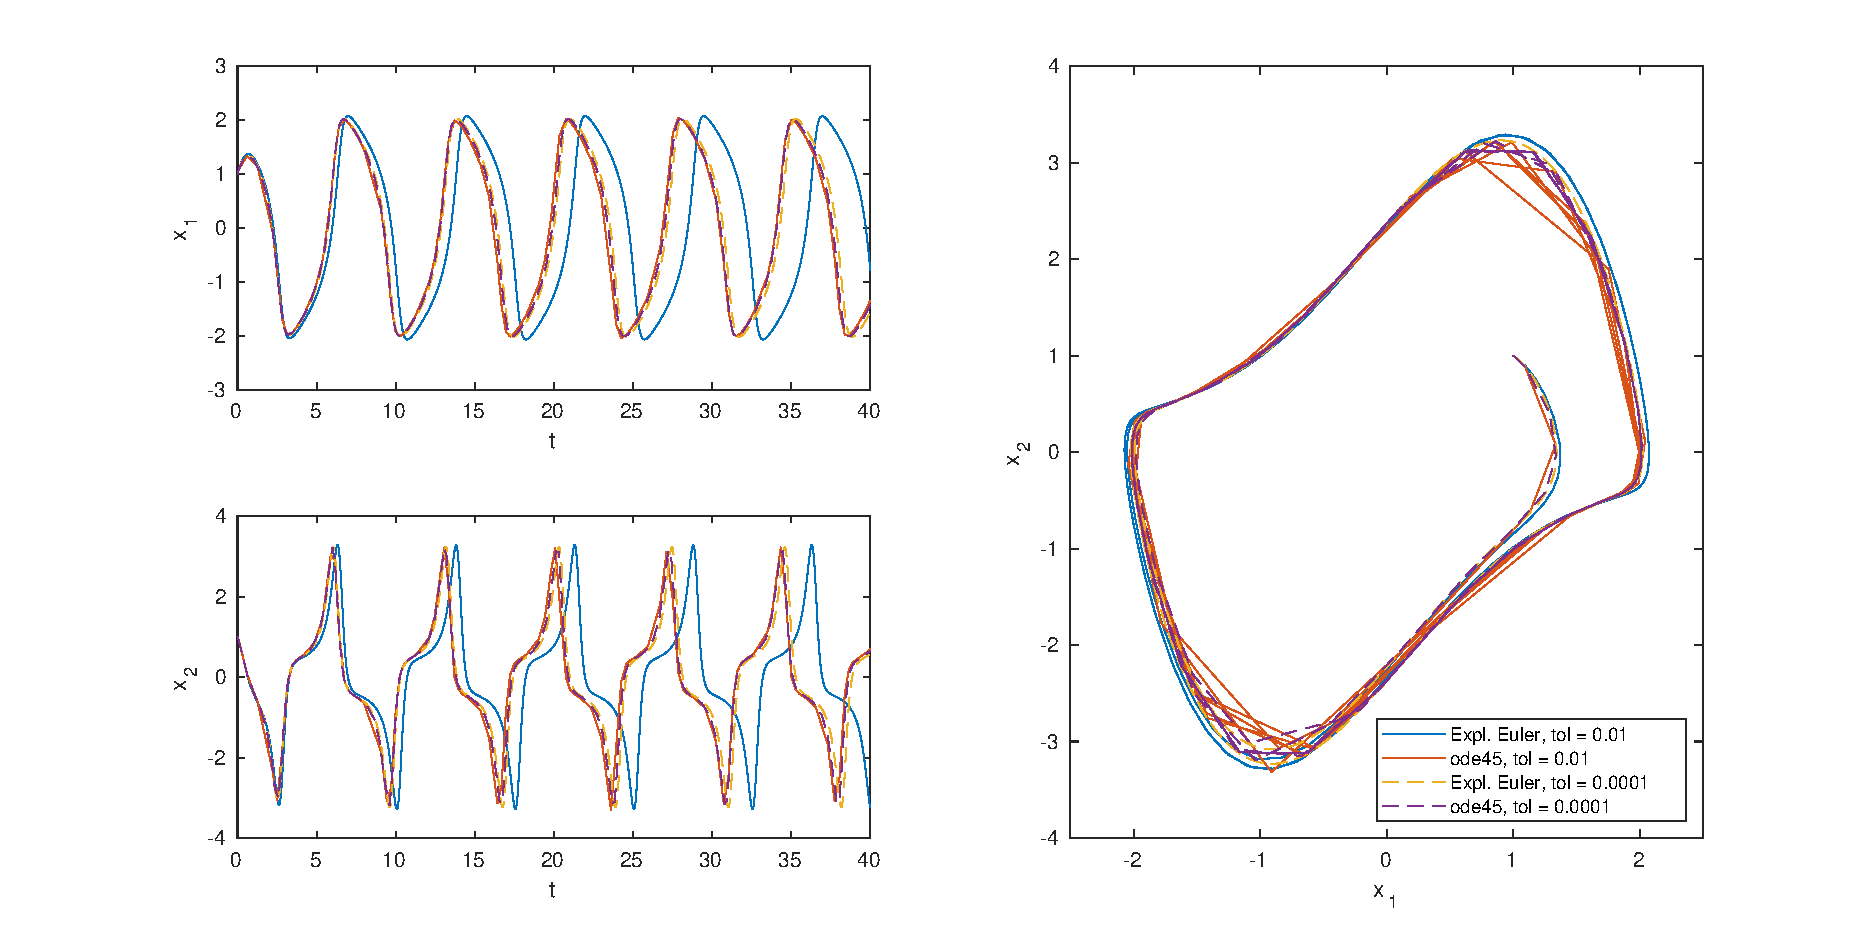
\includegraphics[width=1.25\textwidth]{images/2/2_6_mu_1_5.pdf}}
    \caption{Solution for the Van der Pol problem ($\mathit{\mu = 1.5}$) using Explicit Euler vs. \code{ode45}}
    \label{2_6_mu_1_5}
\end{figure}

\begin{table}[H]
    \centering
    \begin{tabular}{@{}l|cc|cc@{}}
    \toprule
    \textbf{Method} & \multicolumn{2}{c|}{\textbf{Expl. Euler}} & \multicolumn{2}{c}{\textbf{ode45}} \\
    Tolerances           & 0.01           & 0.0001          & 0.01       & 0.0001       \\ \midrule
    Function evaluations & 853            & 7383            & 787        & 1357         \\
    Calculated steps     & 473            & 3695            & 131        & 226          \\
    Accepted steps       & 380            & 3688            & 100        & 180          \\
    Rejected steps       & 93             & 7               & 31         & 46           \\ \bottomrule
    \end{tabular}
    \caption{Parameters of the Explicit Euler vs. \code{ode45} for the Van der Pol problem ($\mathit{\mu = 1.5}$)}
    \label{2_6_adaptive_mu_1_5_table}
\end{table}

\begin{figure}[H]
    \centering
    \makebox[\textwidth][c]{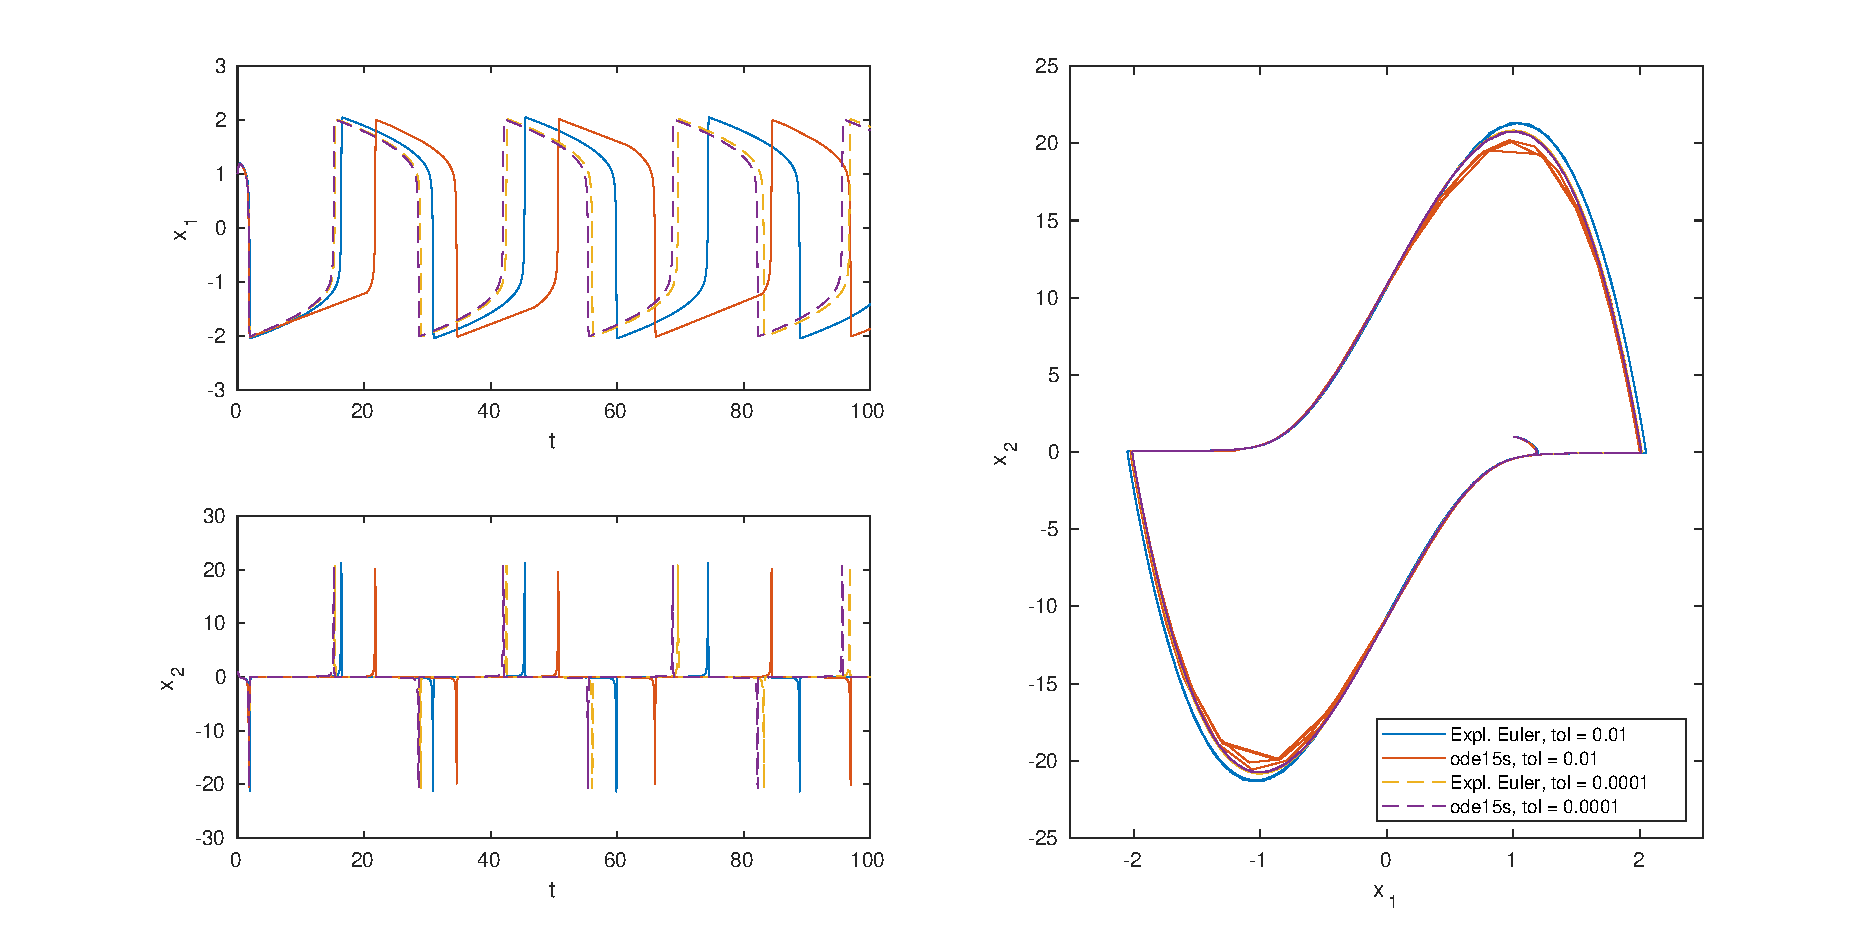
\includegraphics[width=1.25\textwidth]{images/2/2_6_mu_15.pdf}}
    \caption{Solution for the Van der Pol problem ($\mathit{\mu = 15}$) using Explicit Euler vs. \code{ode15s}}
    \label{2_6_mu_15}
\end{figure}

\begin{table}[H]
    \centering
    \begin{tabular}{@{}l|ll|ll@{}}
    \toprule
    \textbf{Method}      & \multicolumn{2}{c|}{\textbf{Expl. Euler}} & \multicolumn{2}{c}{\textbf{ode15s}} \\
    Tolerances           & 0.01               & 0.0001               & 0.01            & 0.0001            \\ \midrule
    Function evaluations & 2108               & 11246                & 1273            & 2780              \\
    Calculated steps     & 1219               & 5740                 & 558             & 1327              \\
    Accepted steps       & 889                & 5506                 & 411             & 1094              \\
    Rejected steps       & 330                & 234                  & 147             & 233               \\ \bottomrule
    \end{tabular}
    \caption{Parameters of the Explicit Euler vs. \code{ode15s} for the Van der Pol problem ($\mathit{\mu = 15}$)}
    \label{2_6_adaptive_mu_15_table}
\end{table}

For the CSTR problem, we also see how both the Explicit Euler and \code{ode45} fail where the problem turns more stiff. The \code{ode15s} achieves very good performance in this case.
\begin{figure}[H]
    \centering
    \begin{subfigure}{0.8\linewidth}
        \centering
        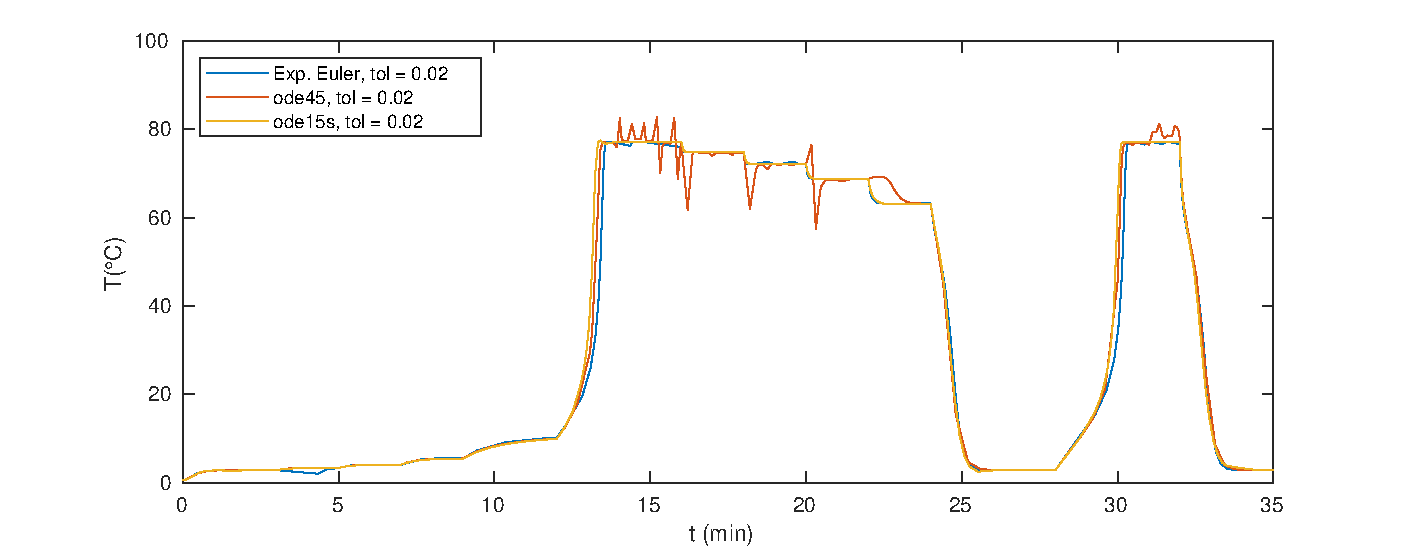
\includegraphics[width=1\linewidth]{images/2/2_6_3D.pdf} 
        \caption{CSTR 3D problem}
    \end{subfigure} \\
    \begin{subfigure}{0.8\linewidth}
        \centering
        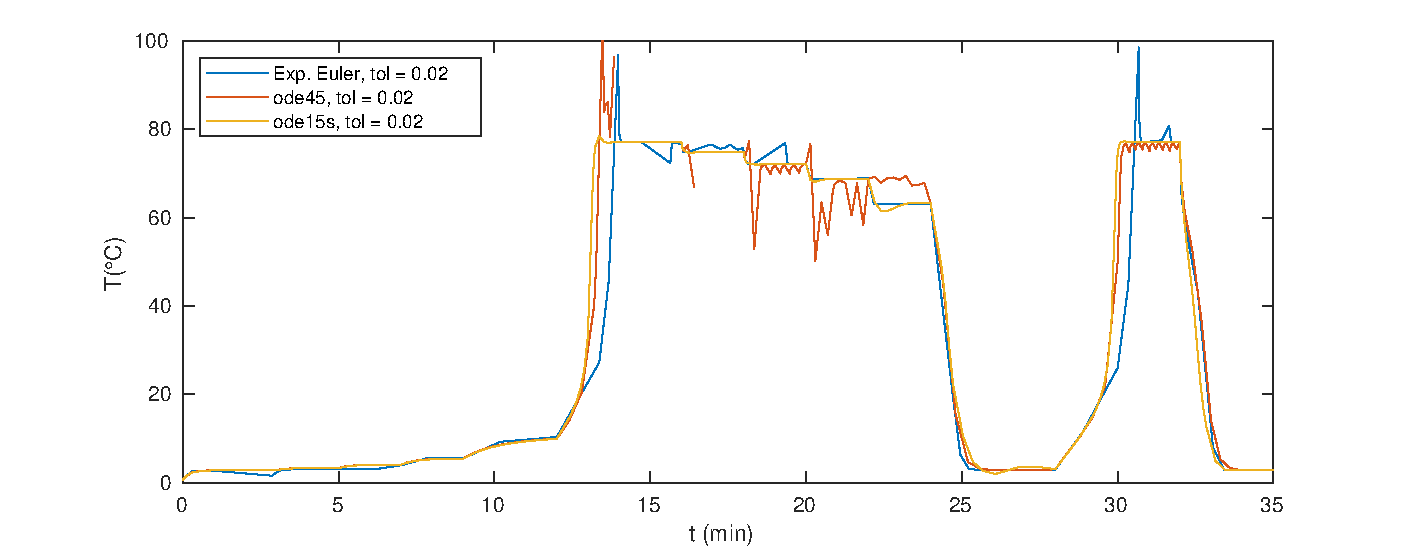
\includegraphics[width=1\linewidth]{images/2/2_6_1D.pdf}
        \caption{CSTR 1D problem}
    \end{subfigure}
    \caption{Solution for the CSTR problem using Explicit Euler vs. \code{ode45} and \code{ode15s}}
    \label{2_6_3D_1D}
\end{figure}

\begin{table}[H]
    \centering
    \begin{tabular}{@{}l|c|c|c@{}}
    \toprule
    \textbf{Method}      & \textbf{Expl. Euler} & \textbf{ode45} & \textbf{ode15s} \\
    Tolerances           & 0.02                 & 0.02           & 0.02            \\ \midrule
    Function evaluations & 291                  & 1477           & 480             \\
    Calculated steps     & 168                  & 1555           & 1423            \\
    Accepted steps       & 123                  & 211            & 203             \\
    Rejected steps       & 45                   & 33             & 27              \\ \bottomrule
    \end{tabular}
    \caption{Parameters of the Explicit Euler vs. \code{ode45} and \code{ode15s} for the CSTR-3D problem}
    \label{2_6_3D_table}
\end{table}

\begin{table}[H]
    \centering
    \begin{tabular}{@{}l|c|c|c@{}}
    \toprule
    \textbf{Method}      & \textbf{Expl. Euler} & \textbf{ode45} & \textbf{ode15s} \\
    Tolerances           & 0.02                 & 0.02           & 0.02            \\ \midrule
    Function evaluations & 201                  & 1297           & 375             \\
    Calculated steps     & 117                  & 1270           & 1275            \\
    Accepted steps       & 84                   & 195            & 180             \\
    Rejected steps       & 33                   & 19             & 27              \\ \bottomrule
    \end{tabular}
    \caption{Parameters of the Explicit Euler vs. \code{ode45} and \code{ode15s} for the CSTR-1D problem}
    \label{2_6_1D_table}
\end{table}

\pagebreak

\section{Implicit ODE solver} \label{part3}
We consider again the initial value problem in (\ref{2_problem}).

\subsection{Describe the implicit Euler algorithm (i.e. provide an algorithm for it in
your report and explain how you get from the differential equations to the
numerical formulas).}
The idea behind the Implicit Euler is that, instead of using the function evaluation at the previous point, it uses the one at the future point. A more mathematical derivation would be to approximate the integral form of the problem by the right-hand rectangle method, as in
\begin{equation*}
    x(t_{n+1})- x(t_n) = \int_{t_n}^{t_{n+1}} f(t,x(t),p) dt \approx hf(t+1,x(t+1),p).
\end{equation*}
As seen in part \ref{part1}, this improves the absolute region of stability of the Explicit Euler considerably. However, the bad news is that a nonlinear system of equations must be solved in each time step. To achieve this we'll use Newton's method to approximate the solution. The Implicit Euler is therefore calculated as:
\begin{align*}
    x_0 &= x(t_0), \\
    x_n &= x_{n-1} + hf(t_n, x_n, p), \hspace{1em} \text{solve } x_n \text{ for } n = 1,2,\ldots, N.
\end{align*}

%%%%%%%%%%%%%%%%%%%%%%%%%%%%%%%%%%%%%%%%%%%%%%%%%%%%%%%%%%%%%%%%%%%%%%%%%%%%%%%%%%%%%%%%%%%%%%%%%%%

\subsection{Implement  an  algorithm  in  Matlab  for  the  implicit  Euler  method  with
 fixed time-step and provide this in your report.  Use a format that enables
syntax highlighting.}

\begin{lstlisting}[caption = Newton's method, captionpos=b, label=3_NewtonsMethod]
 function [x,k] = NewtonsMethod(FunJac, tk, xk, h, xinit, tol, maxit, args)
k = 0;
t = tk + h;
x = xinit;
[f,J] = feval(FunJac,t,x,args{:});
k = k + 1;
R = x - h*f - xk;
I = eye(length(xk));

while( (k<maxit) && (norm(R,'inf')>tol) )
    dRdx = I - J*h;
    dx = dRdx\R;
    x = x - dx;
    [f,J] = feval(FunJac,t,x,args{:});
    k = k+1;
    R = x - h*f - xk;
end

\end{lstlisting}
\begin{lstlisting}[caption = Implicit Euler method with fixed time step size, captionpos=b, label=3_ImEuler_fixed]
function [T,X] = EulerImplicit_fixed(funJac, tspan, h, x0, args)

t0 = tspan(1);
tf = tspan(end);
T = t0:h:tf;
N = size(T,2);
X = zeros(size(x0,1), N);
X(:,1) = x0;

tol = 1.0e-8;
maxit = 100;

for k=1:N-1
    f = feval(funJac,T(k),X(:,k),args{:});
    xinit = X(:,k) + f*h;
    [X(:,k+1),~] = NewtonsMethod(funJac, T(:,k), X(:,k), h, xinit, tol, maxit, args);
end
end

\end{lstlisting}
%%%%%%%%%%%%%%%%%%%%%%%%%%%%%%%%%%%%%%%%%%%%%%%%%%%%%%%%%%%%%%%%%%%%%%%%%%%%%%%%%%%%%%%%%%%%%%%%%%%

\subsection{ Implement  an  algorithm  in  Matlab  for  the  implicit  Euler  method  with
adaptive time step and error estimation using step doubling.}
The Implicit Euler with adaptive time step will also call Newton's method shown in Listing \ref{3_NewtonsMethod}
\begin{lstlisting}[caption = Implicit Euler method with fixed time step size, captionpos=b, label=3_ImEuler_adaptive]
function [T,X,r_out,h_out,info] = EulerImplicit_adaptive(funJac,tspan,h0,x0,abstol,reltol,args)

epstol = 0.8;
facmin = 0.1;
facmax = 5.0;

newtontol = 1.0e-8;
maxit = 100;

t0 = tspan(1);
tf = tspan(end);
t = t0;
h = h0;
x = x0;

T = t0;
X = x0;
r_out = [];
h_out = [h0];
info = zeros(1,4);

nfun = 0;
nstep = 0;
naccept = 0;

while t < tf
    if (t+h > tf)
        h = tf-t;
    end
    [f,J] = feval(funJac,t,x,args{:});
    nfun = nfun + 1;
    
    AcceptStep = false;
    while ~AcceptStep
        % Single step size
        xinit1 = x + h*f;
        [x1,nfun_local] = NewtonsMethod(funJac, t, x, h, xinit1, newtontol, maxit, args);
        nfun = nfun + nfun_local;
        
        hm = 0.5*h;
        tm = t + hm;
        xinitm = x + hm*f;
        [xm,nfun_local] = NewtonsMethod(funJac, t, x, hm, xinitm, newtontol, maxit, args);
        nfun = nfun + nfun_local;
        
        [fm,Jm] = feval(funJac,tm,xm,args{:});
        nfun = nfun + 1;
        xinit1hat = xm + hm*f;
        [x1hat,nfun_local] = NewtonsMethod(funJac, tm, xm, hm, xinit1hat, newtontol, maxit, args);
        nfun = nfun + nfun_local;
        
        nstep = nstep + 1;
        
        e = abs(x1hat-x1);
        r = max(e./max(abstol, abs(x1hat) .* reltol));
        AcceptStep = (r <= 1.0);
        
        if AcceptStep
            t = t+h;
            x = x1hat;
            
            T = [T,t];
            X = [X,x];
            r_out = [r_out, r];
            h_out = [h_out, h];
            naccept = naccept + 1;
        end
        
        h = max(facmin, min(sqrt(epstol/r), facmax)) * h;
    end
end

info(1) = nfun;
info(2) = nstep;
info(3) = naccept;
info(4) = nstep - naccept;

end

\end{lstlisting}

%%%%%%%%%%%%%%%%%%%%%%%%%%%%%%%%%%%%%%%%%%%%%%%%%%%%%%%%%%%%%%%%%%%%%%%%%%%%%%%%%%%%%%%%%%%%%%%%%%%

\subsection{Test your algorithms on the Van der Pol problem \texorpdfstring{($\mathbf{\mu = 2}$ and $\mathbf{\mu = 12}$, $\mathbf{x_0 = [0.5;0.5]}$).}{(mu = 2 and mu = 12, x0 = [0.5;0.5]).}}
The way of calling the ODE solvers is similar as in Exercise \ref{2_4}. Results are shown in the following Figures and Tables. First thing we can notice when looking at the plot is that the Implicit, contrary to the Explicit, approximates the error from the inside of the steady-state curve: worst approximations of the solution make the frequency of the oscillation larger and the amplitude smaller.

We can also observe the stiffness of $\mu=12$ is handled a lot better. Specially in Figure \ref{3_4_adaptive_mu_12}, while there's still some oscillations when $x_2$ shifts suddenly, it is considerably better than the Explicit. It's also worth noticing, looking at Tables \ref{3_4_adaptive_mu_2_table} and \ref{3_4_adaptive_mu_12_table}, the huge increase in the number of function evaluations. This is obviously due to the added call to Newton's method to solve the non linear equation.

\begin{figure}[H]
    \centering
    \makebox[\textwidth][c]{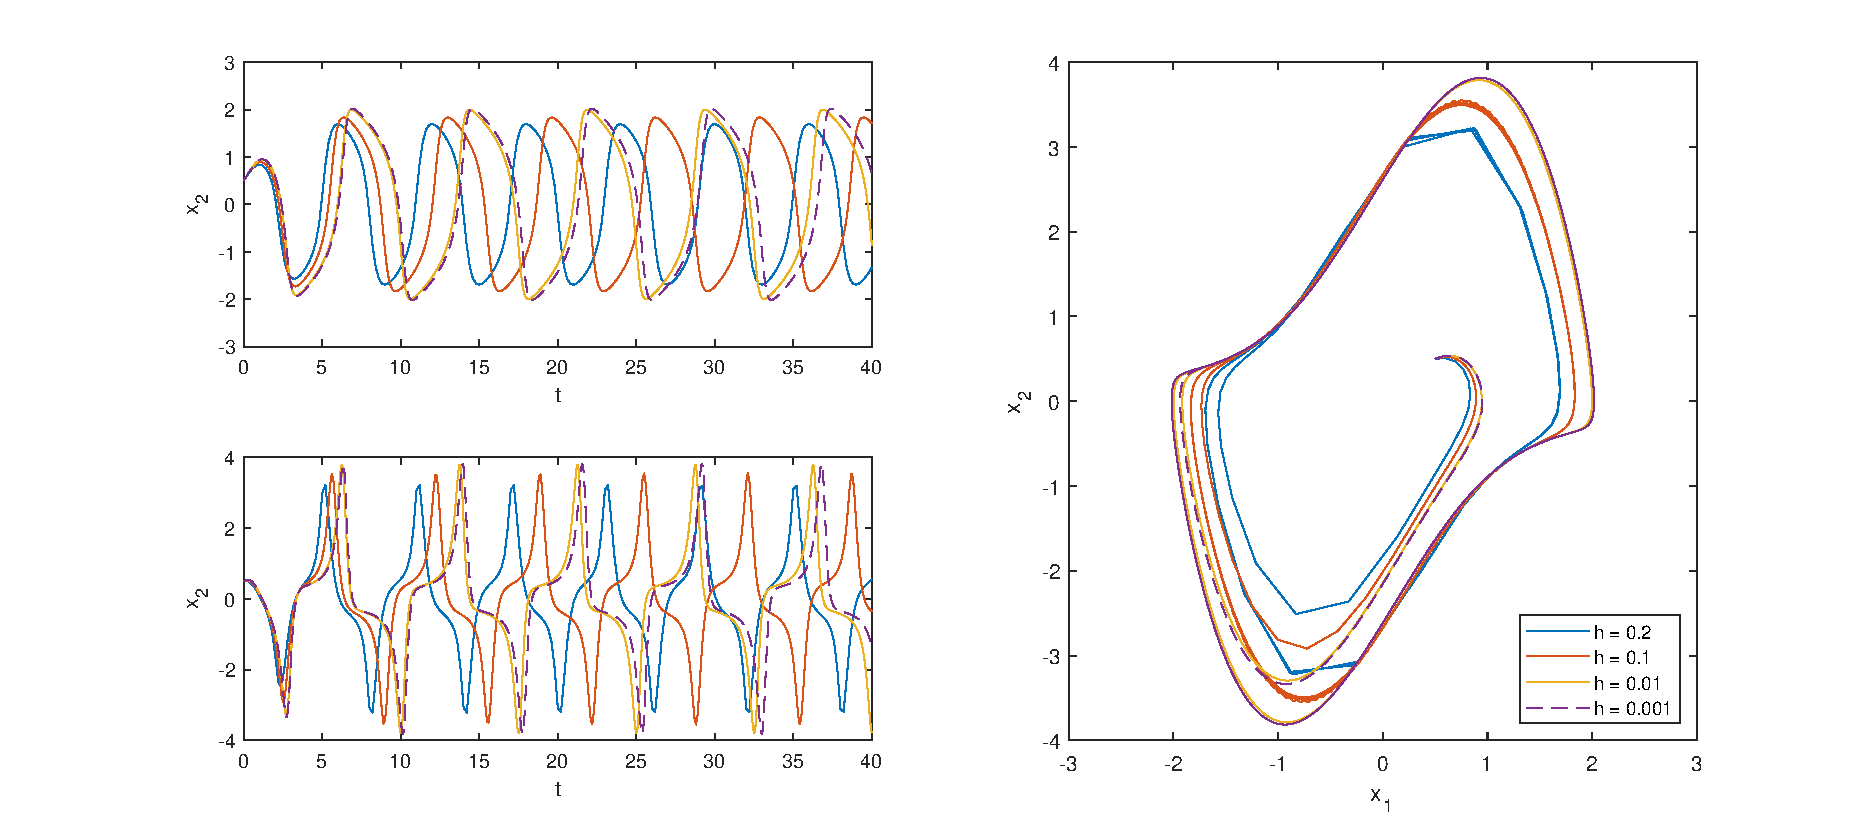
\includegraphics[width=1.25\textwidth]{images/3/3_4_fixed_mu_2.pdf}}
    \caption{Solution for the Van der Pol problem ($\mathit{\mu = 2}$) using Implicit Euler with fixed step size}
    \label{3_4_fixed_mu_2}
\end{figure}

\begin{figure}[H]
    \centering
    \makebox[\textwidth][c]{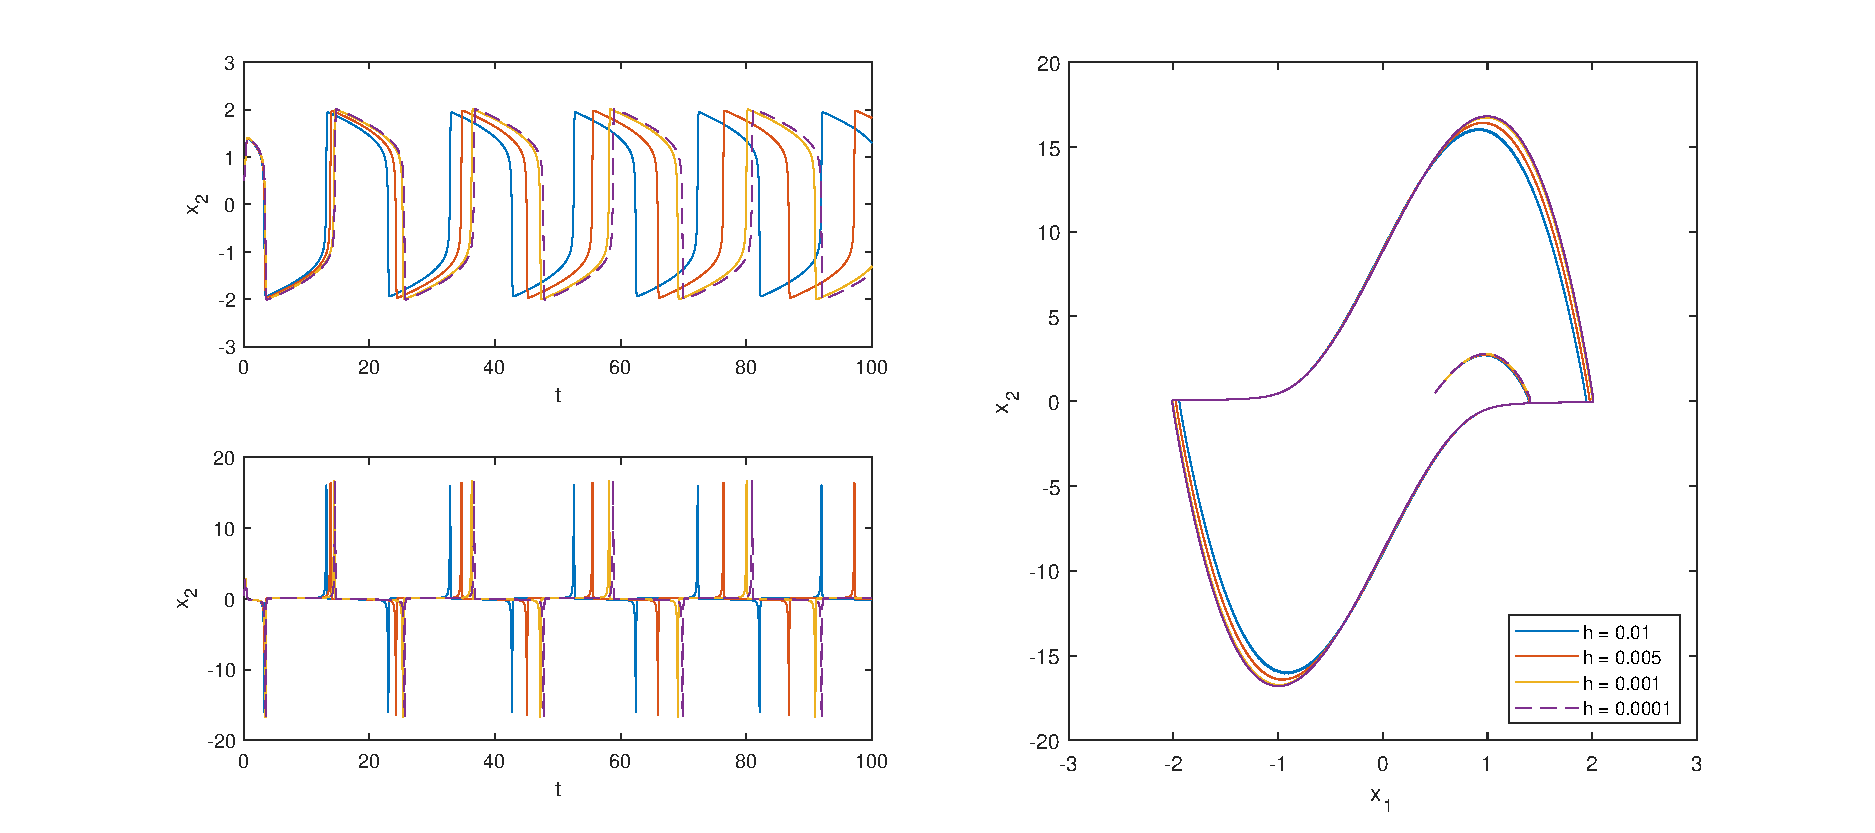
\includegraphics[width=1.25\textwidth]{images/3/3_4_fixed_mu_12.pdf}}
    \caption{Solution for the Van der Pol problem ($\mathit{\mu = 12}$) using Implicit Euler with fixed step size}
    \label{3_4_fixed_mu_12}
\end{figure}

\begin{figure}[H]
    \centering
    \makebox[\textwidth][c]{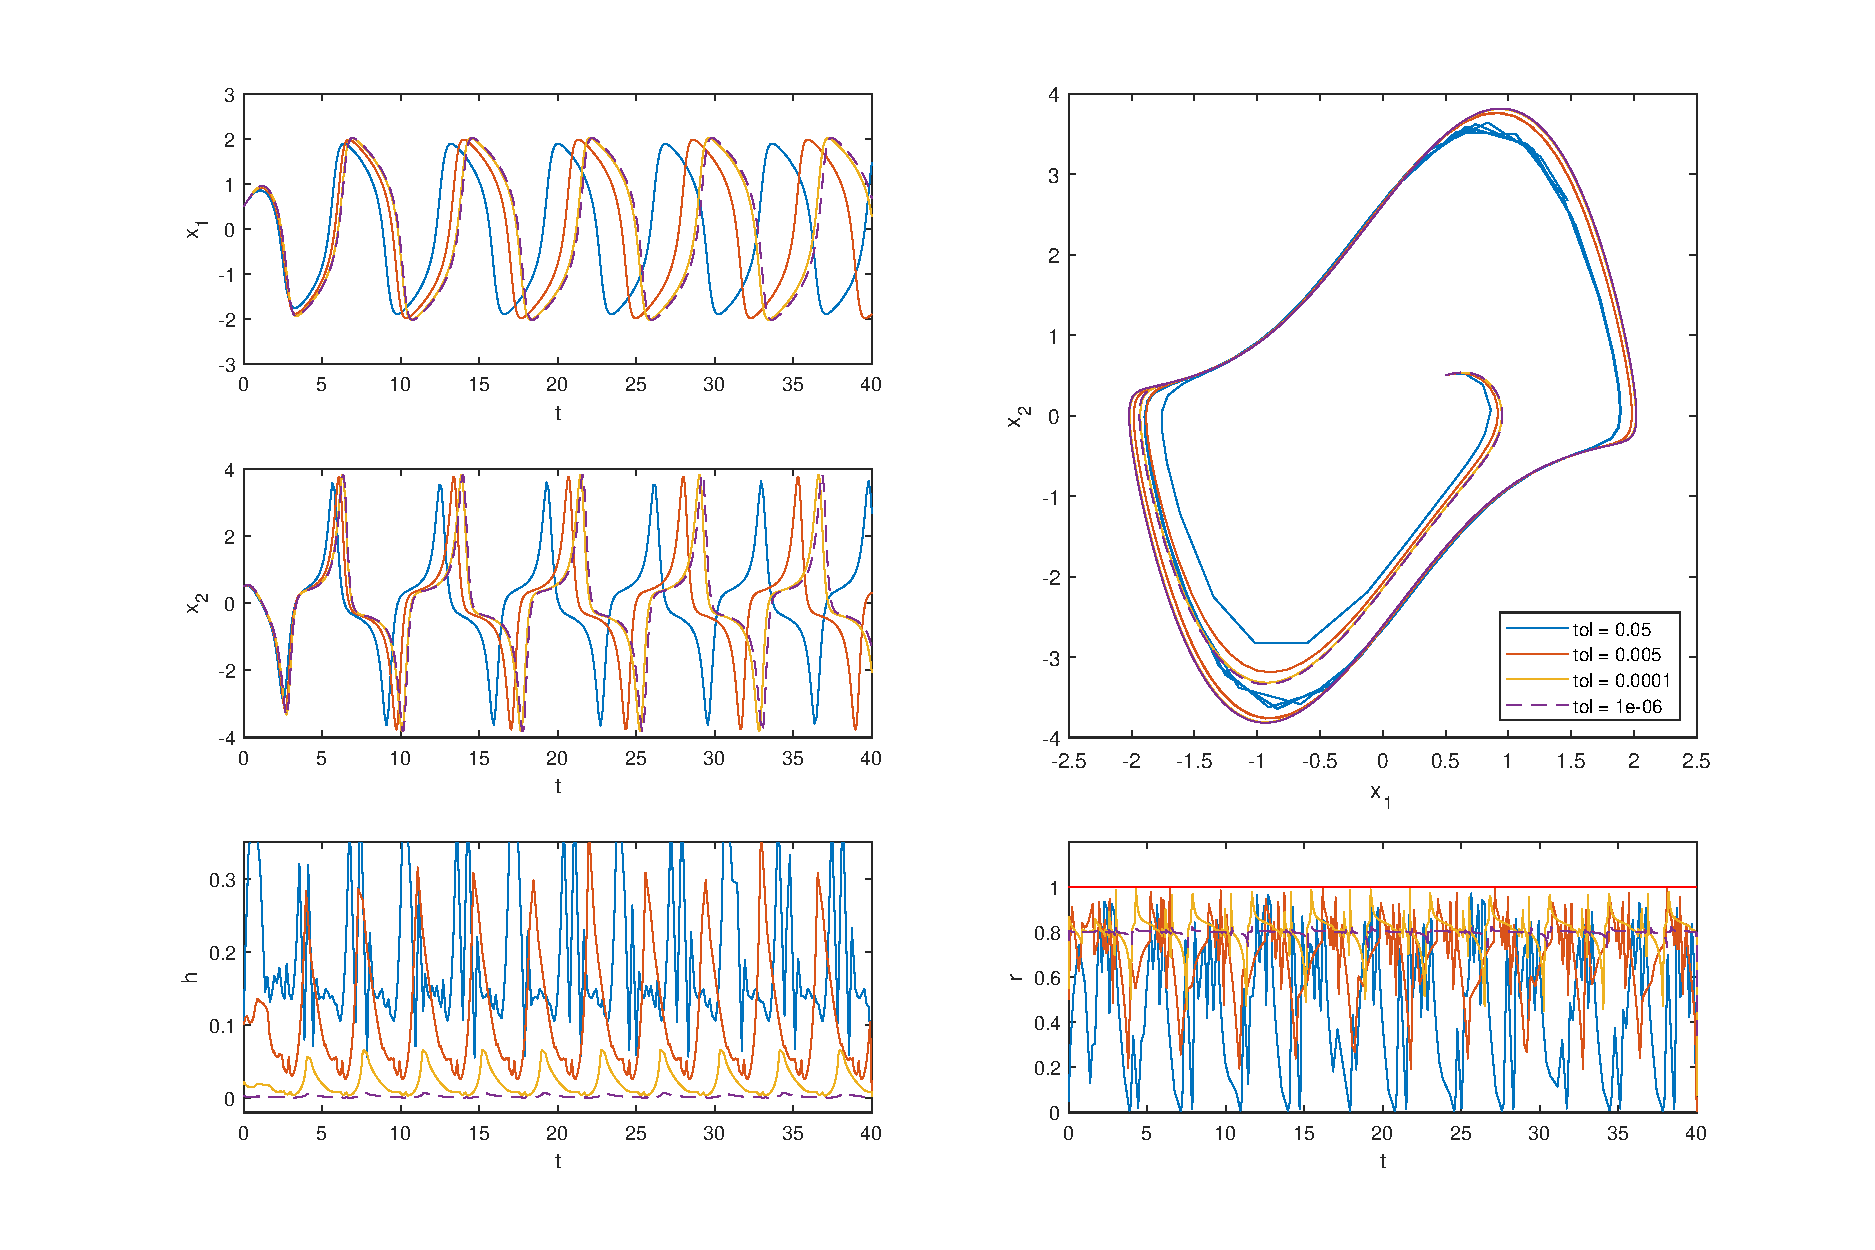
\includegraphics[width=1.25\textwidth]{images/3/3_4_adaptive_mu_2.pdf}}
    \caption{Solution for the Van der Pol problem ($\mathit{\mu = 2}$) using Implicit Euler with adaptive step size}
    \label{3_4_adaptive_mu_2}
\end{figure}

\begin{table}[H]
    \centering
    \begin{tabular}{@{}l|cccc@{}}
    \toprule
    Tolerances           & 0.05 & 0.005 & 0.0001 & 1e-06      \\ \midrule
    Function evaluations & 5732 & 8162  & 30764  & 3.0379e+05 \\
    Calculated steps     & 353  & 754   & 3799   & 37974      \\
    Accepted steps       & 237  & 589   & 3797   & 37972      \\
    Rejected steps       & 116  & 165   & 2      & 2          \\ \bottomrule
    \end{tabular}
    \caption{Parameters of the Implicit Euler with adaptive step size for the Van der Pol problem ($\mathit{\mu = 2}$)}
    \label{3_4_adaptive_mu_2_table}
\end{table}

\begin{figure}[H]
    \centering
    \makebox[\textwidth][c]{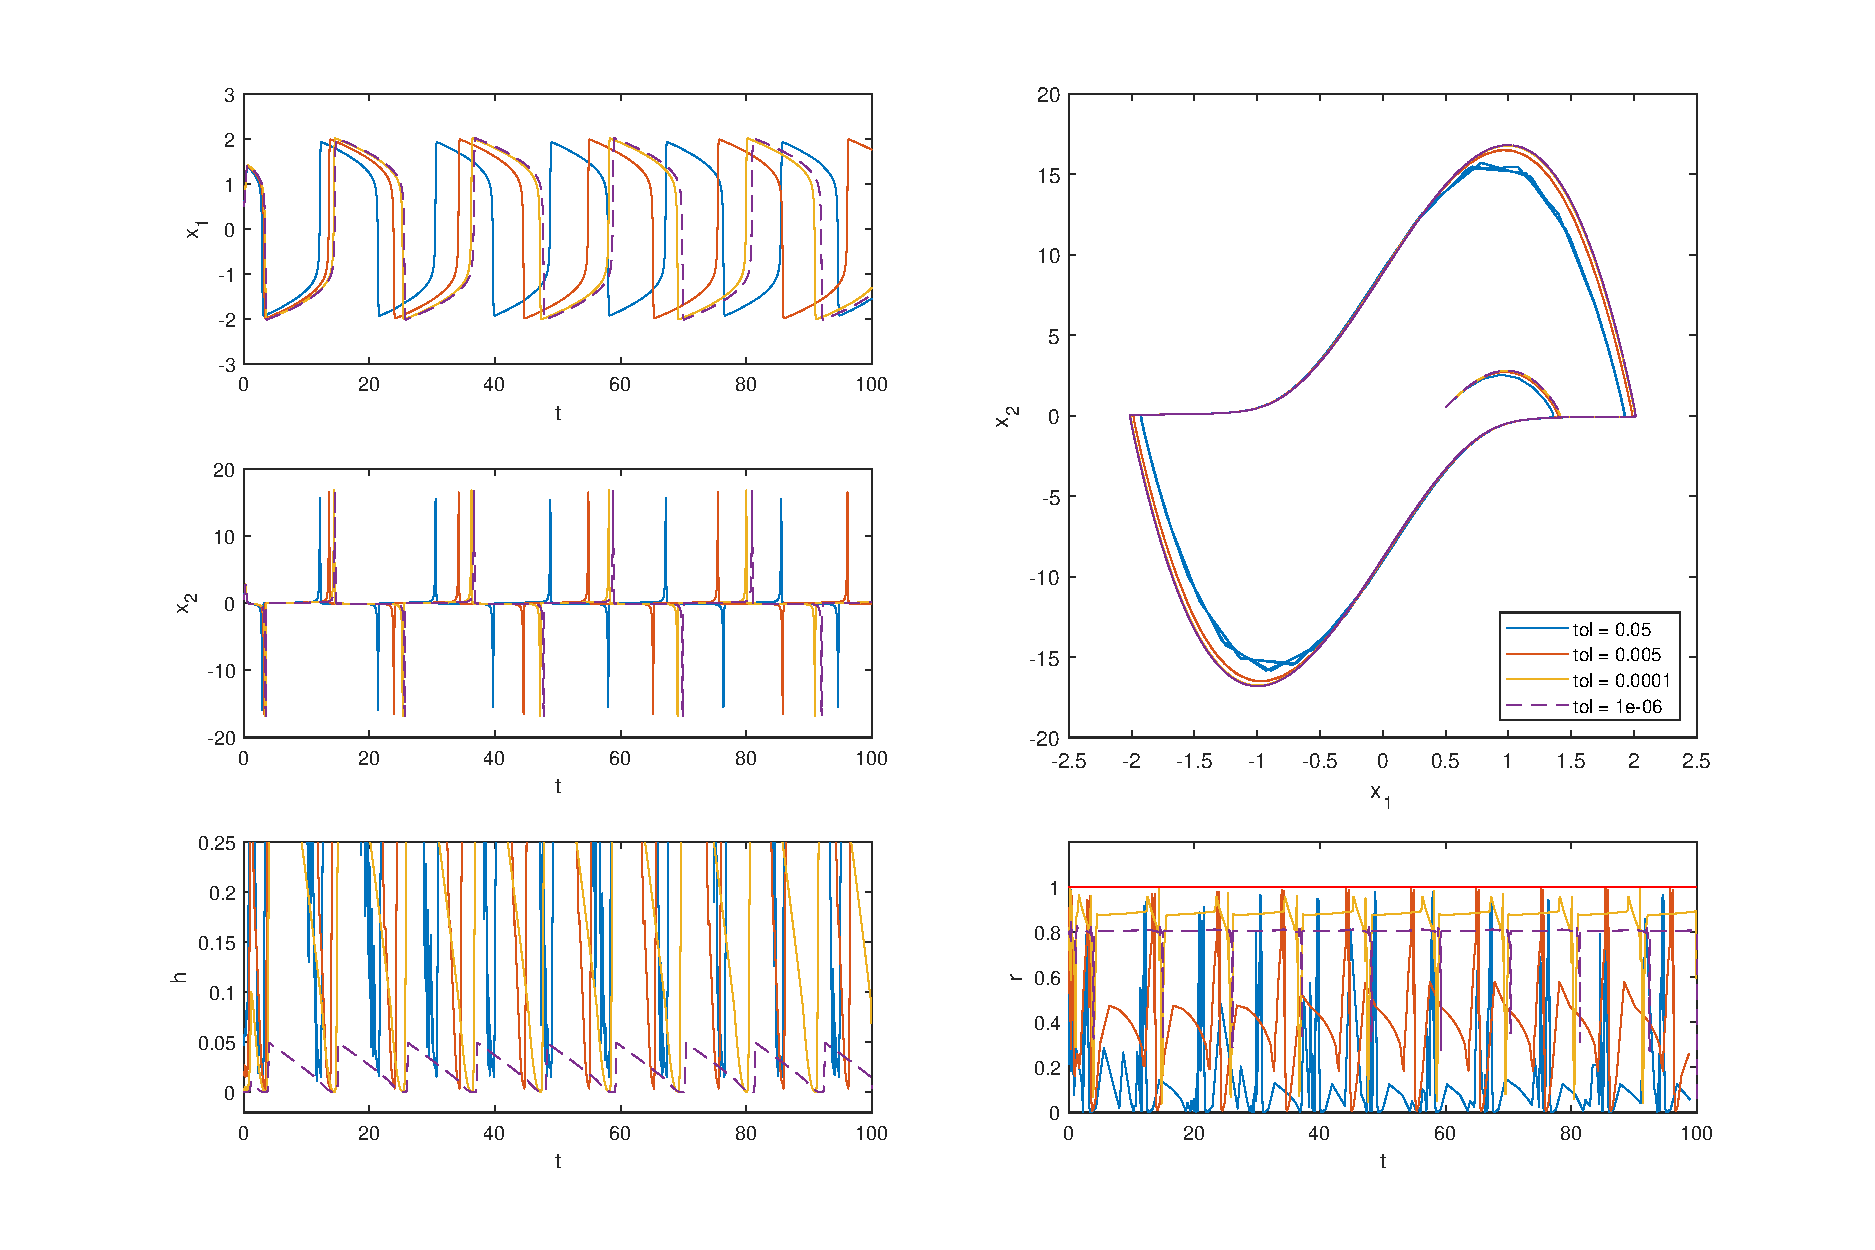
\includegraphics[width=1.25\textwidth]{images/3/3_4_adaptive_mu_12.pdf}}
    \caption{Solution for the Van der Pol problem ($\mathit{\mu = 12}$) using Implicit Euler with adaptive step size}
    \label{3_4_adaptive_mu_12}
\end{figure}

\begin{table}[H]
    \centering
    \begin{tabular}{@{}l|cccc@{}}    \toprule
    Tolerances           & 0.05  & 0.005 & 0.0001 & 1e-06      \\ \midrule
    Function evaluations & 24307 & 14368 & 48124  & 4.6157e+05 \\
    Calculated steps     & 776   & 1288  & 5746   & 57695      \\
    Accepted steps       & 478   & 982   & 5739   & 57692      \\
    Rejected steps       & 298   & 306   & 7      & 3          \\ \bottomrule
    \end{tabular}
    \caption{Parameters of the Implicit Euler with adaptive step size for the Van der Pol problem ($\mathit{\mu = 12}$)}
    \label{3_4_adaptive_mu_12_table}
\end{table}

\pagebreak
%%%%%%%%%%%%%%%%%%%%%%%%%%%%%%%%%%%%%%%%%%%%%%%%%%%%%%%%%%%%%%%%%%%%%%%%%%%%%%%%%%%%%%%%%%%%%%%%%%%

\subsection{Test  your  algorithms  on  the  adiabatic  CSTR  problem  described  in  the
papers uploaded to Learn (3D-version and 1D-version).}
Here are shown the results of the Implicit Euler for the CSTR problem. Just as in last exercise, we can't observe any significant difference between the 3D and 1D problem (Figure \ref{3_5_3D_vs_1D}). The results when working with a fixed time step size (Figure \ref{3_5_3D_1D_hs}) are the same for both results. We can observe how the implicit manages to control the \textit{stiffness} of the problem when the values of $F$ go lower, we can't find no longer the oscillations. The highest step size misses completely the values though. However, it converges quicker than the explicit to the real solution.

For the adaptive method, the value \code{facmax} was set to be $1.5$, otherwise the asymptotic step controller was too sensible and diverged a lot. Here, we can see that the step size controller is working and the results converge quickly to the real solution. The 1D solution misses the larger values of $T$ (when $F$ is lower) for the largest tolerance. 
\begin{figure}[H]
    \centering
    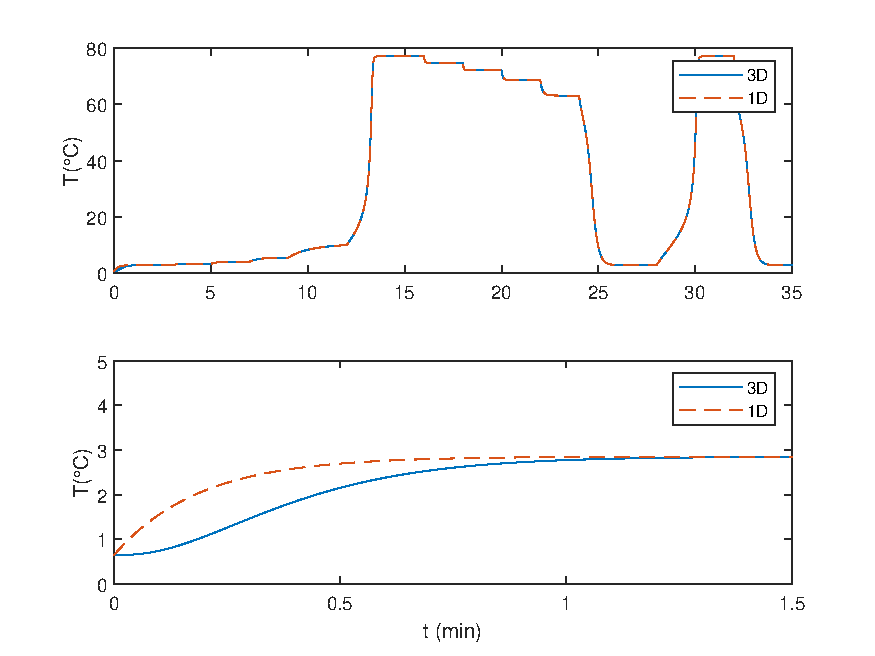
\includegraphics[width=0.8\textwidth]{images/3/3_5_3D_vs_1D.pdf}
    \caption{Comparison of the solutions for the CSTR 3D and 1D with Implicit Euler}
    \label{3_5_3D_vs_1D}
\end{figure}

\begin{figure}[H]
\centering
    \begin{subfigure}{0.8\linewidth}
        \centering
        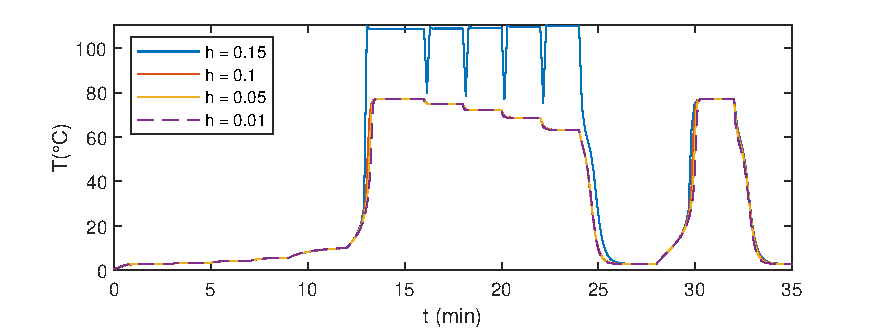
\includegraphics[width=1\linewidth]{images/3/3_5_3D_hs.pdf} 
        \caption{CSTR 3D problem}
    \end{subfigure} \\
    \begin{subfigure}{0.8\linewidth}
        \centering
        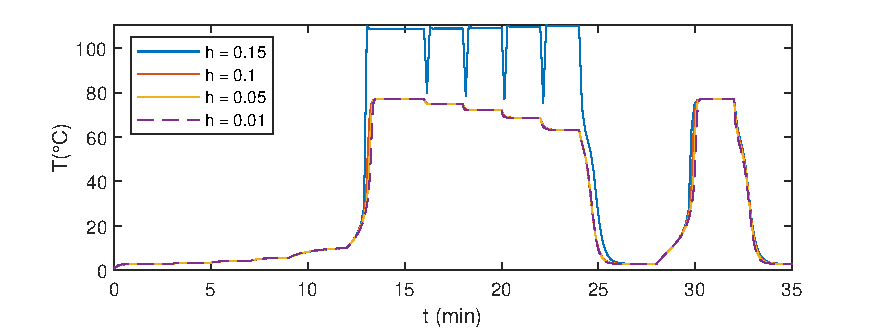
\includegraphics[width=1\linewidth]{images/3/3_5_1D_hs.pdf}
        \caption{CSTR 1D problem}
    \end{subfigure}
    \caption{Solution for the CSTR problem using Implicit Euler with fixed step size}
    \label{3_5_3D_1D_hs}
\end{figure}

\begin{figure}[H]
    \centering
    \makebox[\textwidth][c]{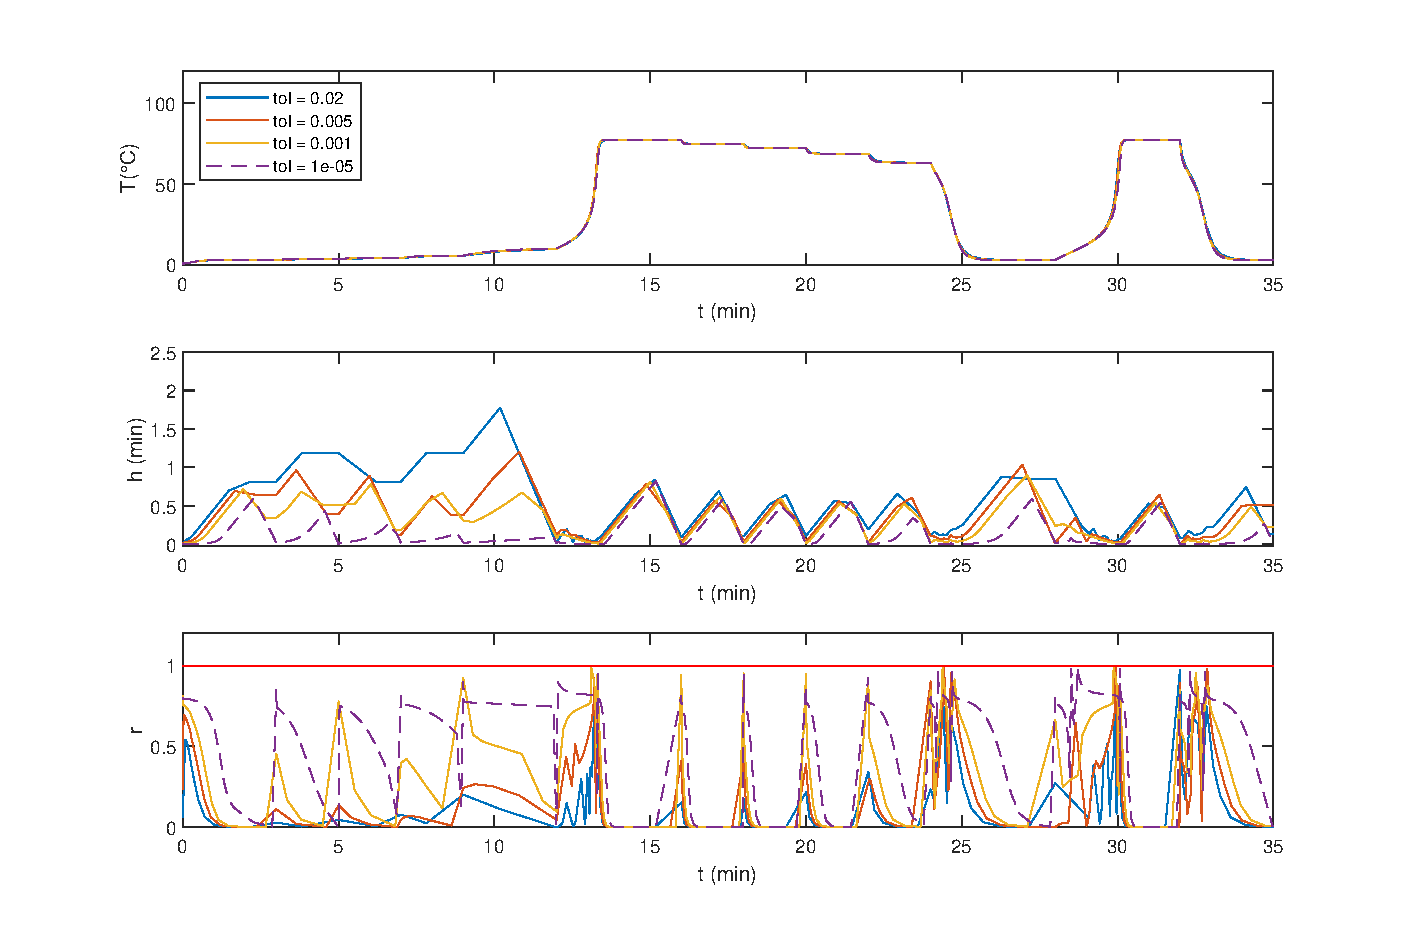
\includegraphics[width=1\textwidth]{images/3/3_5_3D_tols.pdf}}
    \caption{Solution for the CSTR 3D problem using Implicit Euler with adaptive step size}
    \label{3_5_3D_tols}
\end{figure}

\begin{table}[H]
    \centering
    \begin{tabular}{@{}l|cccc@{}}
    \toprule
    Tolerances           & 0.02 & 0.005 & 0.001 & 1e-05 \\ \midrule
    Function evaluations & 2386 & 3171  & 4325  & 21476 \\
    Calculated steps     & 146  & 232   & 388   & 2589  \\
    Accepted steps       & 121  & 188   & 307   & 2537  \\
    Rejected steps       & 25   & 44    & 81    & 52    \\ \bottomrule
    \end{tabular}
    \caption{Parameters of the Implicit Euler with adaptive step size for the CSTR 3D problem}
    \label{3_5_3D_tols_table}
\end{table}

\begin{figure}[H]
    \centering
    \makebox[\textwidth][c]{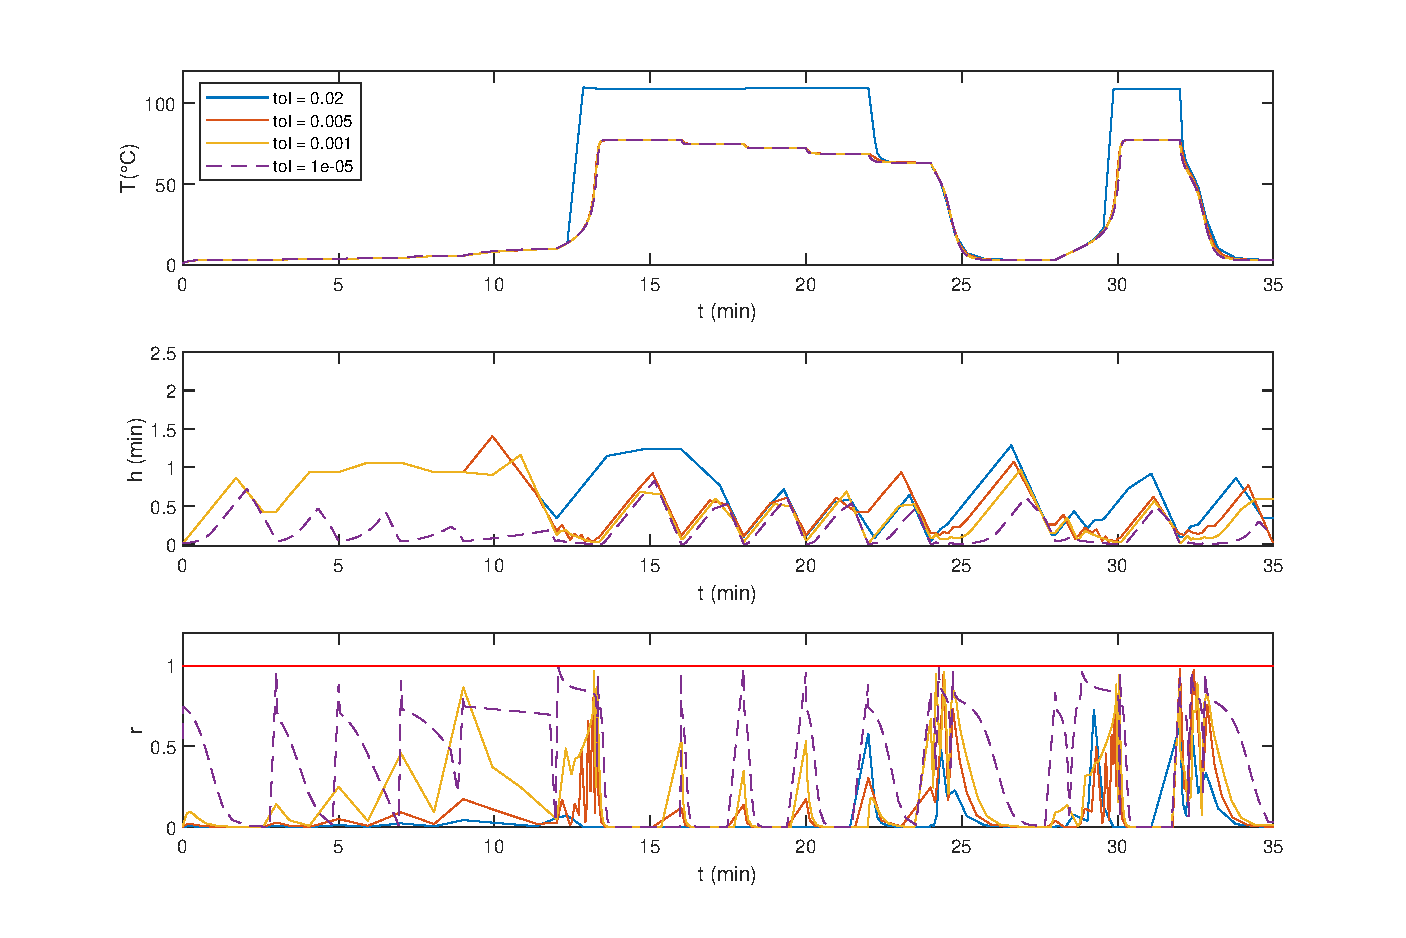
\includegraphics[width=1\textwidth]{images/3/3_5_1D_tols.pdf}}
    \caption{Solution for the CSTR 1D problem using Implicit Euler with adaptive step size}
    \label{3_5_1D_tols}
\end{figure}

\begin{table}[H]
    \centering
    \begin{tabular}{@{}l|cccc@{}}
    \toprule
    Tolerances           & 0.02 & 0.005 & 0.001 & 1e-05 \\ \midrule
    Function evaluations & 2311 & 2592  & 3144  & 11390 \\
    Calculated steps     & 88   & 141   & 222   & 1126  \\
    Accepted steps       & 80   & 115   & 173   & 1073  \\
    Rejected steps       & 8    & 26    & 49    & 53    \\ \bottomrule
    \end{tabular}
    \caption{Parameters of the Implicit Euler with adaptive step size for the CSTR 1D problem}
    \label{3_5_1D_tols_table}
\end{table}

%%%%%%%%%%%%%%%%%%%%%%%%%%%%%%%%%%%%%%%%%%%%%%%%%%%%%%%%%%%%%%%%%%%%%%%%%%%%%%%%%%%%%%%%%%%%%%%%%%%

\subsection{Compare the results from your algorithms with the results you get using some  of  Matlab's  ODE  solvers  The  report  should  contain  figures  and  a discussion of your algorithm for different tolerances and step sizes.}
For the Van der Pol problem, we tested Implicit Euler against \code{ode45} for the non-stiff case ($\mu = 1.5$), and against \code{ode15s} for the stiff case ($\mu = 15$). Contrary to what we obtained using explicit Euler, the Implicit Euler works fine in the stiff case, even though the \code{ode15s} achieves better accuracy with a fewer no. of function evaluations. This is also due to the fact that we're using step doubling to approximate the error. In the non-stiff case, however, the no. of evaluations is ridiculously high compared to the \code{ode45}, which makes sense given that it's an implicit method vs. an explicit one in a non-stiff problem.

\begin{figure}[H]
    \centering
    \makebox[\textwidth][c]{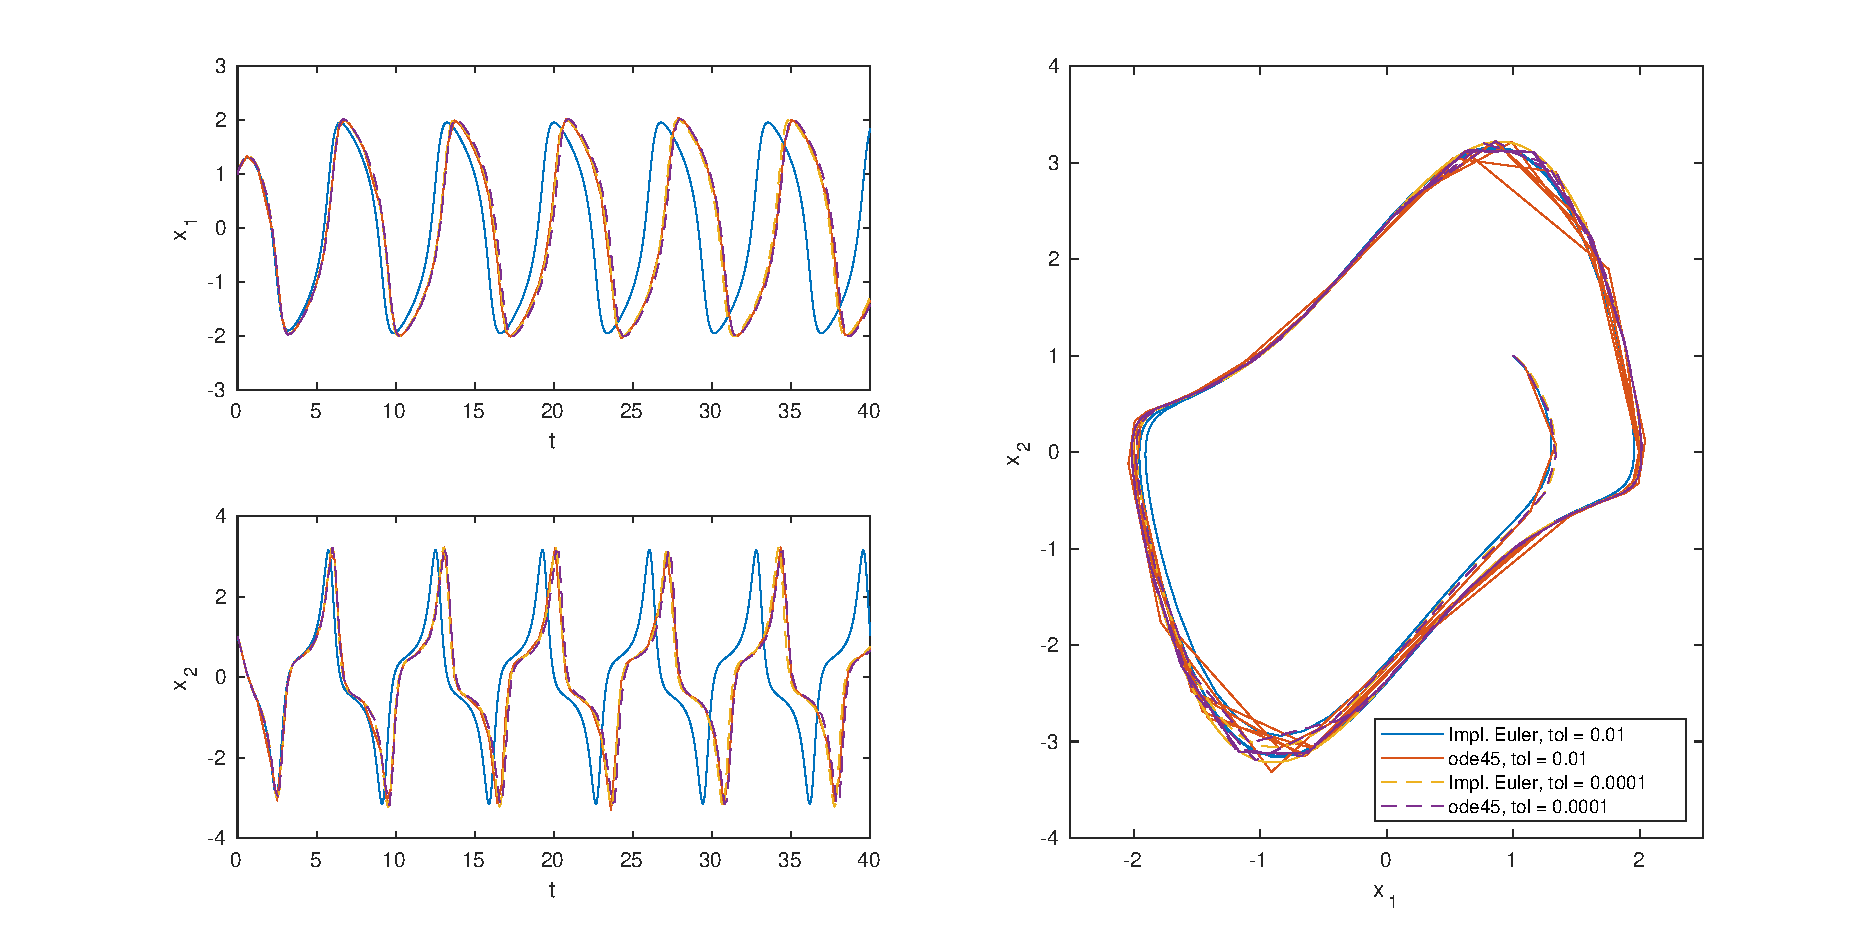
\includegraphics[width=1.25\textwidth]{images/3/3_6_mu_1_5.pdf}}
    \caption{Solution for the Van der Pol problem ($\mathit{\mu = 1.5}$) using Implicit Euler vs. \code{ode45}}
    \label{3_6_mu_1_5}
\end{figure}

\begin{table}[H]
    \centering
    \begin{tabular}{@{}l|cc|cc@{}}
    \toprule
    \textbf{Method}      & \multicolumn{2}{c|}{\textbf{Impl. Euler}} & \multicolumn{2}{c}{\textbf{ode45}} \\
    Tolerances           & 0.01               & 0.0001               & 0.01            & 0.0001           \\ \midrule
    Function evaluations & 5713               & 29600                & 787             & 1357             \\
    Calculated steps     & 522                & 3666                 & 131             & 226              \\
    Accepted steps       & 402                & 3664                 & 100             & 180              \\
    Rejected steps       & 120                & 2                    & 31              & 46               \\ \bottomrule
    \end{tabular}
    \caption{Parameters of the Implicit Euler vs. \code{ode45} for the Van der Pol problem ($\mathit{\mu = 1.5}$)}
    \label{3_6_adaptive_mu_1_5_table}
\end{table}

\begin{figure}[H]
    \centering
    \makebox[\textwidth][c]{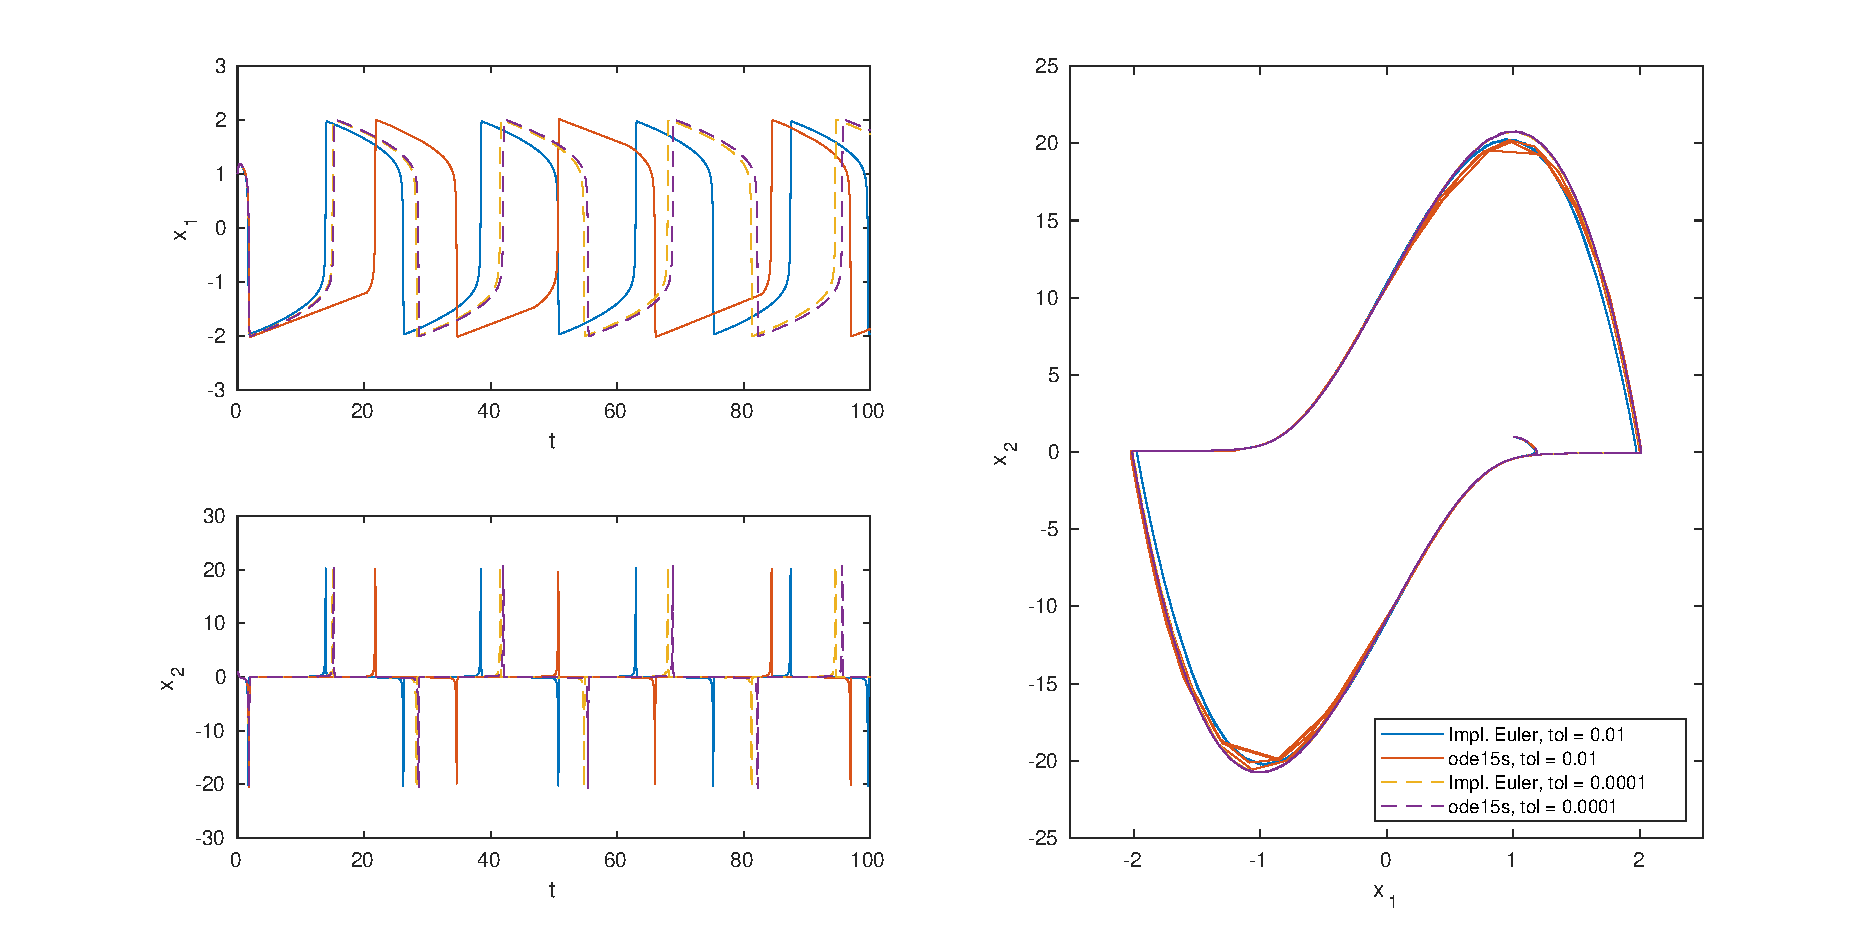
\includegraphics[width=1.25\textwidth]{images/3/3_6_mu_15.pdf}}
    \caption{Solution for the Van der Pol problem ($\mathit{\mu = 15}$) using Implicit Euler vs. \code{ode15s}}
    \label{3_6_mu_15}
\end{figure}

\begin{table}[H]
    \centering
    \begin{tabular}{@{}l|ll|ll@{}}
    \toprule
    \textbf{Method}      & \multicolumn{2}{c|}{\textbf{Impl. Euler}} & \multicolumn{2}{c}{\textbf{ode15s}} \\
    Tolerances           & 0.01                & 0.0001              & 0.01            & 0.0001            \\ \midrule
    Function evaluations & 12508               & 43567               & 1273            & 2780              \\
    Calculated steps     & 937                 & 5198                & 558             & 1327              \\
    Accepted steps       & 743                 & 5189                & 411             & 1094              \\
    Rejected steps       & 120                 & 2                   & 147             & 233               \\ \bottomrule
    \end{tabular}
    \caption{Parameters of the Implicit Euler vs. \code{ode15s} for the Van der Pol problem ($\mathit{\mu = 15}$)}
    \label{3_6_adaptive_mu_15_table}
\end{table}

For the CSTR problem, we also see how both the Implicit Euler and \code{ode15s} achieve good performance for the 3D case. For the 1D case we see the Implicit deviating a bit, but this could be caused by the tolerance being too wide. The \code{ode45} achieves worse performance in both cases.

\begin{figure}[H]
    \centering
    \begin{subfigure}{0.8\linewidth}
        \centering
        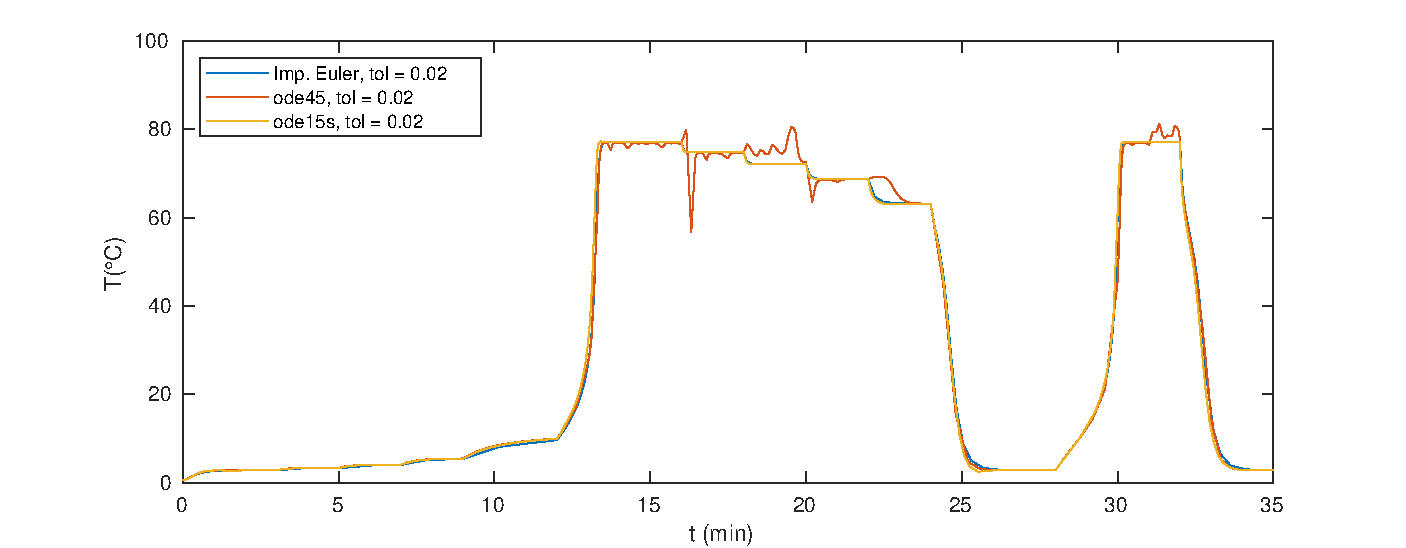
\includegraphics[width=1\linewidth]{images/3/3_6_3D.pdf} 
        \caption{CSTR 3D problem}
    \end{subfigure} \\
    \begin{subfigure}{0.8\linewidth}
        \centering
        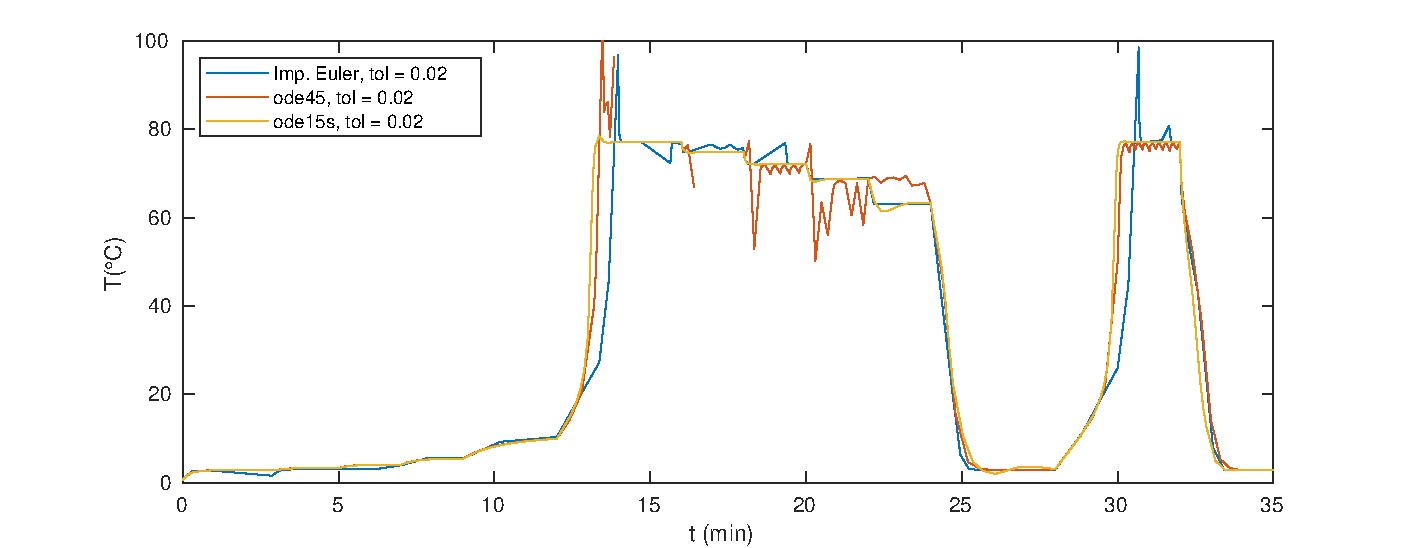
\includegraphics[width=1\linewidth]{images/3/3_6_1D.pdf}
        \caption{CSTR 1D problem}
    \end{subfigure}
    \caption{Solution for the CSTR problem using Implicit Euler vs. \code{ode45} and \code{ode15s}}
    \label{3_6_3D_1D}
\end{figure}

\begin{table}[H]
    \centering
    \begin{tabular}{@{}l|c|c|c@{}}
    \toprule
    \textbf{Method}      & \textbf{Impl. Euler} & \textbf{ode45} & \textbf{ode15s} \\
    Tolerances           & 0.02                 & 0.02           & 0.02            \\ \midrule
    Function evaluations & 2386                 & 1513           & 477             \\
    Calculated steps     & 146                  & 1586           & 1408            \\
    Accepted steps       & 121                  & 220            & 201             \\
    Rejected steps       & 25                   & 30             & 29              \\ \bottomrule
    \end{tabular}
    \caption{Parameters of the Implicit Euler vs. \code{ode45} and \code{ode15s} for the CSTR-3D problem}
    \label{3_6_3D_table}
\end{table}

\begin{table}[H]
    \centering
    \begin{tabular}{@{}l|c|c|c@{}}
    \toprule
    \textbf{Method}      & \textbf{Impl. Euler} & \textbf{ode45} & \textbf{ode15s} \\
    Tolerances           & 0.02                 & 0.02           & 0.02            \\ \midrule
    Function evaluations & 201                  & 1297           & 375             \\
    Calculated steps     & 117                  & 1270           & 1275            \\
    Accepted steps       & 84                   & 195            & 180             \\
    Rejected steps       & 33                   & 19             & 27              \\ \bottomrule
    \end{tabular}
    \caption{Parameters of the Implicit Euler vs. \code{ode45} and \code{ode15s} for the CSTR-1D problem}
    \label{3_6_1D_table}
\end{table}

\pagebreak
%%%%%%%%%%%%%%%%%%%%%%%%%%%%%%%%%%%%%%%%%%%%%%%%%%%%%%%%%%%%%%%%%%%%%%%%%%%%%%%%%%%%%%%%%%%%%%%%%%%

\subsection{Discuss when one should use the implicit Euler method rather than the
explicit Euler method and illustrate that using an example.}
As previously discussed, the Implicit Euler method is a lot more robust than the Explicit, this is, it handles \textit{stiff problems} a lot better. The reason behind this behaviour is connected to the \textit{region of stability} of the method. We showed the region of stability for the Explicit and Implicit Euler in Figure \ref{stability_regions}. The problem can require an extremely low $h$ for the Explicit Method in order to satisfy $|y_{n-1}| \leq |y_n|$. The implicit, being A-stable, doesn't have this problem.

If we solve the Van der Pol problem for $\mu = 100$ with Explicit and Implicit method with adaptive step we will observe this behaviour. Both will be solved with a tolerance of $10^{-3}$. Just by looking at the $h$ vs. time and $r$ vs. time we can notice the difference. Notice that the time step with the Explicit must be really small even though the solution is really smooth. Otherwise, it would explode. The Implicit manages the stiffness a lot better, getting to values of time step of more than $8$ units of time. The solution is equally valid in both of them. Looking at table \ref{3_7_table}, we notice that the number of steps calculated is more than $10$ times smaller on the implicit. In this case, the Implicit proves to be computationally better, even though we are calling the Newton method at every time step. 

\begin{figure}[H]
    \centering
    \makebox[\textwidth][c]{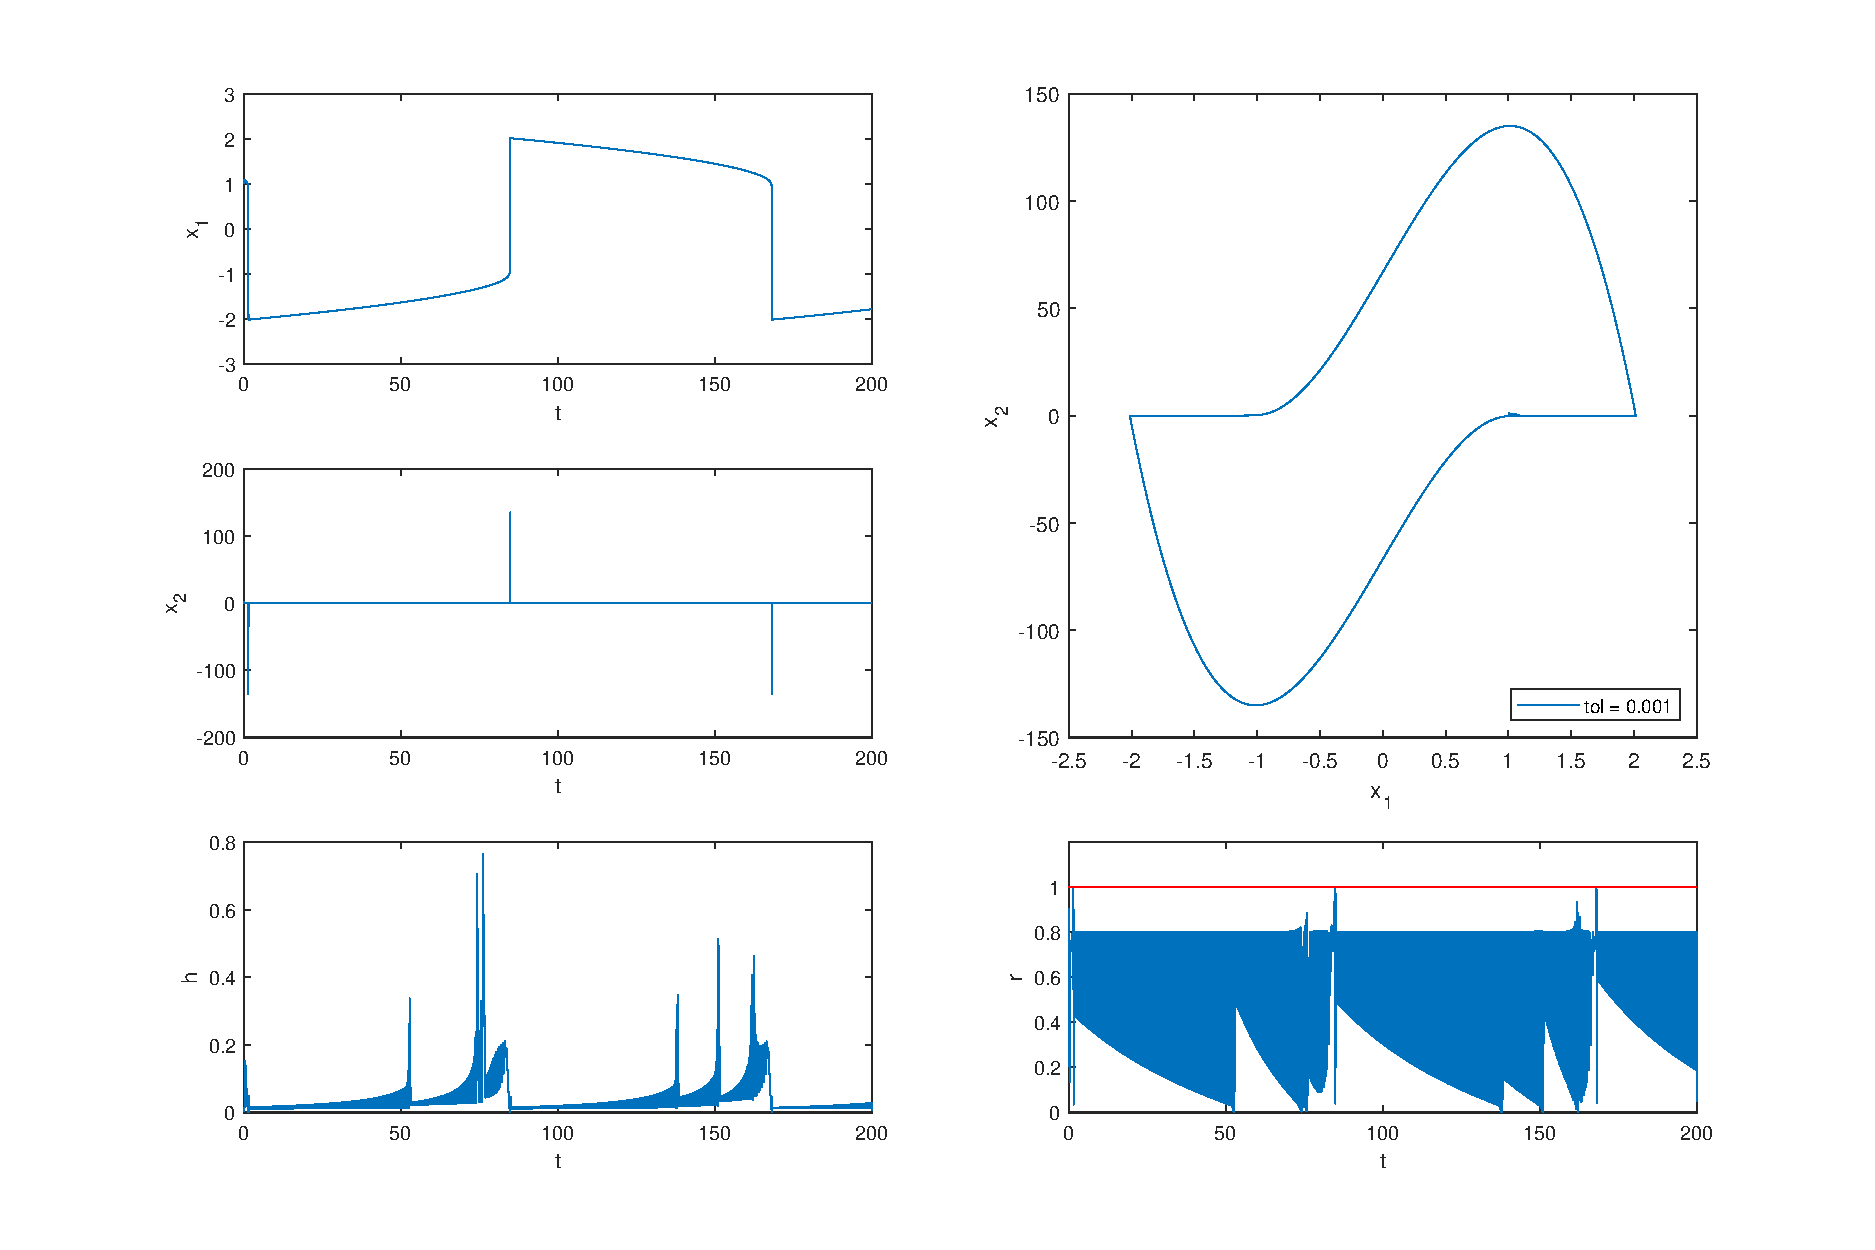
\includegraphics[width=1.25\textwidth]{images/3/3_7_explicit.pdf}}
    \caption{Solution for the Van der Pol problem ($\mathit{\mu = 100}$) using Explicit Euler with adaptive step size}
    \label{3_7_explicit}
\end{figure}

\begin{figure}[H]
    \centering
    \makebox[\textwidth][c]{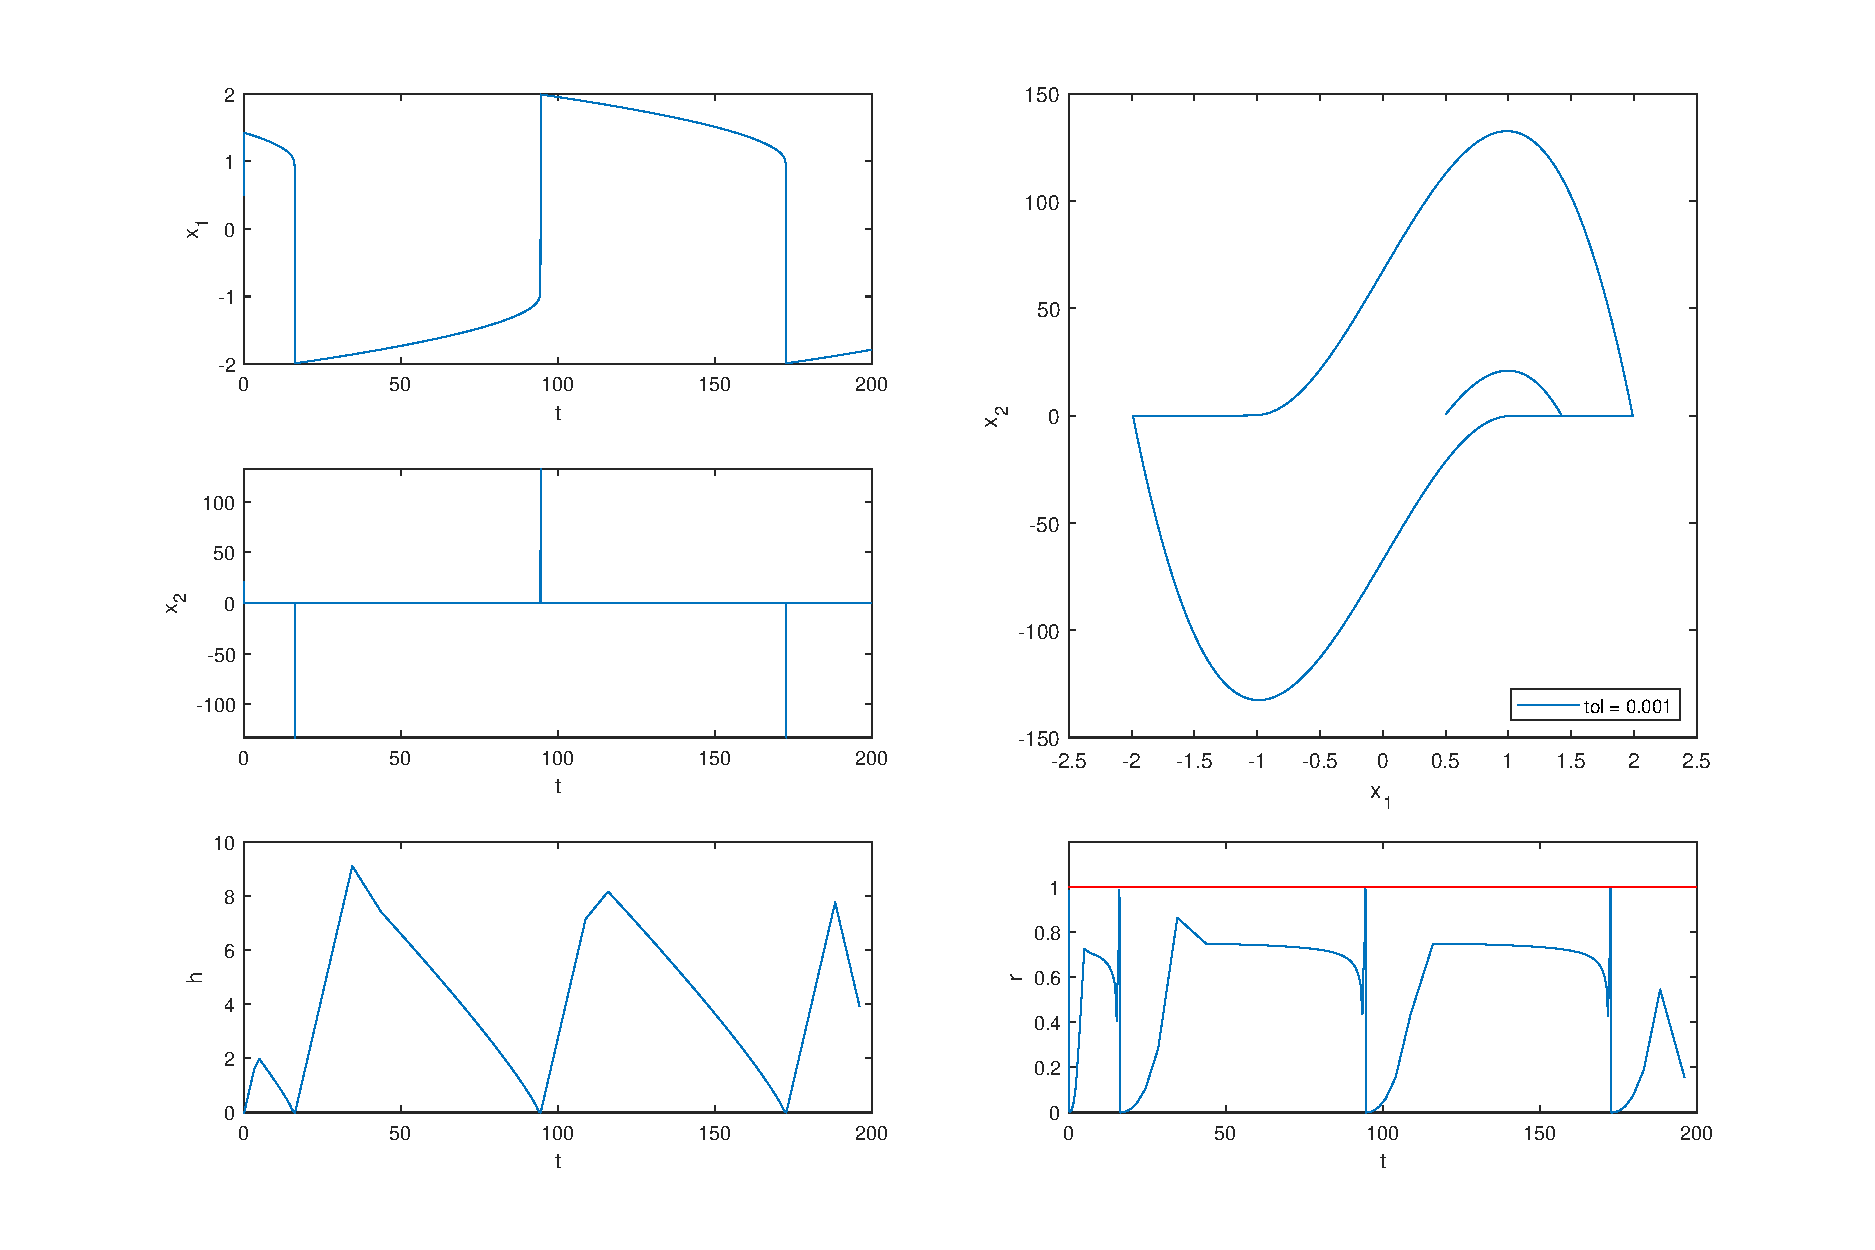
\includegraphics[width=1.25\textwidth]{images/3/3_7_implicit.pdf}}
    \caption{Solution for the Van der Pol problem ($\mathit{\mu = 100}$) using Implicit Euler with adaptive step size}
    \label{3_7_implicit}
\end{figure}

\begin{table}[H]
\centering
\begin{tabular}{@{}l|cc@{}}
\toprule
Tolerances           & Explicit & Implicit \\ \midrule
Function evaluations & 22654    & 12407    \\
Calculated steps     & 13450    & 1207     \\
Accepted steps       & 9204     & 1076     \\
Rejected steps       & 4246     & 131      \\ \bottomrule
\end{tabular}
\caption{Parameters of the Explicit and Implicit methods for the Van der Pol problem ($\mu = 100$)}
\label{3_7_table}
\end{table}
\pagebreak

\section{Solvers for SDEs}
We consider now stochastic differential equations in the form
\begin{equation} \label{4_problem}
    dx(t) = f(t,x(t),p_f) dt + g(t,x(t),p_g) d\omega (t), \hspace{1em} d \omega (t) \sim \mathcal{N}_{iid}(0, Idt)
\end{equation}
where $x \in \mathbb{R}^{n_x}$ and $\omega$ is a stochastic variable with dimension $n_w$, $p_f$ and $p_g$ are parameters for $f:\mathbb{R} \times \mathbb{R}^{n_x} \times \mathbb{R}^{n_{p_f}} \to \mathbb{R}^{n_x}$ and $g:\mathbb{R} \times \mathbb{R}^{n_x} \times \mathbb{R}^{n_{p_g}} \to \mathbb{R}^{n_x \times n_w}$ (i.e. the result of $g$ is a matrix of size $n_x \times n_w$).

\subsection{Make a function in Matlab that can realize a multivariate standard Wiener process.}
We implement the Wiener process in the following function. This generates \code{Ns} realizations of a Wiener process of size \code{nW}.

\begin{lstlisting}[caption = Multivariate standard Wiener process, captionpos=b, label=4_wiener]
function [Tw,W,dW] = StdWienerProcess(tspan,h,nW,Ns,seed)

if nargin == 4
    rng(seed);
end

t0 = tspan(1);
tf = tspan(2);

Tw = t0:h:tf;
N = size(Tw,2);

dW = sqrt(h)*randn(nW,N,Ns);
W  = [zeros(nW,1,Ns) cumsum(dW,2)];
W = W(:,1:end-1,:);
end

\end{lstlisting}
\subsection{Implement the explicit-explicit method with fixed step size.}
\begin{lstlisting}[caption = Euler-Maruyama Method, captionpos=b, label=4_EulerMaruyama]
function [T,X] = EulerMaruyama(ffun,gfun,tspan,h,x0,nW,args)
t0 = tspan(1);
tf = tspan(end);
T = t0:h:tf;
N  = size(T,2);

X  = zeros(size(x0,1),N);
X(:,1) = x0;

[~,~,dW] = StdWienerProcess(tspan,h,nW,1);

for k=1:N-1
    f = feval(ffun,T(k),X(:,k),args{:});
    g = feval(gfun,T(k),X(:,k),args{:});

    psi = X(:,k) + g*dW(:,k);

    X(:,k+1) = psi + h*f;
end

\end{lstlisting}

\pagebreak

\subsection{Implement the implicit-explicit method with fixed step size.}
\begin{lstlisting}[caption = Newton's Method for SDEs, captionpos=b, label=4_NewtonsMethodSDE]
function [x,f,J] = NewtonsMethodSDE(ffun,t,h,psi,xinit,tol,maxit,args)
I = eye(length(xinit));
x = xinit;

[f,J] = feval(ffun,t,x,args{:});
R = x - h*f - psi;
it = 1;

while ( (norm(R,'inf')>tol) &&(it<= maxit) )
    dRdx = I - J*h;
    mdx = dRdx\R;

    x   = x - mdx;
    [f,J] = feval(ffun,t,x,args{:});
    R = x - h*f - psi;
    it = it + 1;
end
end
\end{lstlisting}

\begin{lstlisting}[caption = Implicit-Explicit Method, captionpos=b, label=4_ImplicitExplicit]
function [T,X] = ImplicitExplicit(ffun,gfun,tspan,h,x0,nW,args)

newtontol = 1e-8;
maxit = 100;

t0 = tspan(1);
tf = tspan(end);
T = t0:h:tf;
N  = size(T,2);

X  = zeros(size(x0,1),N);
X(:,1) = x0;

[~,~,dW] = StdWienerProcess(tspan,h,nW,1);
k = 1;

f = feval(ffun,T(k),X(:,k),args{:});
for k=1:N-1
    g = feval(gfun,T(k),X(:,k),args{:});

    psi = X(:,k) + g*dW(:,k);

    xinit = psi + h*f;
    [X(:,k+1),f,~] = NewtonsMethodSDE(ffun,T(:,k+1),h,psi,xinit,newtontol,maxit,args);
end
end

\end{lstlisting}

\subsection{ Describe your implementations and the idea you use in deriving the methods.  Provide Matlab code for your implementations.}
The idea behind the Euler-Maruyama and Implicit-Explicit is the same as in the Explicit and Implicit Euler already described in Parts \ref{part2} and \ref{part3}, for the function $f$. The problem is that now we also have a function $g$ associated to the Wiener process and, as in order to calculate it we need to discretize it, we just use the Explicit Euler for $g$ both in Euler-Maruyama and Implicit-Explicit. Notice that the Newton's method for SDEs is slightly different to the one already presented in Listing \ref{3_NewtonsMethod}. The Matlab code is already provided in the last two questions.

\pagebreak

\subsection{Test your implementations using SDE versions of the Van der Pol problem.}
We will test the implementations in two SDE versions of the Van der Pol problem. One with \textit{state independent diffusion}:
\begin{align*}
    dx_1(t) &= x_2(t)dt, \\
    dx_2(t) &= \left[ \mu (1-x_1(t)^2)x_2(t) - x_1(t) \right] dt + \sigma d\omega (t),
\end{align*}
and another one with \textit{state dependent diffusion}:
\begin{align*}
    dx_1(t) &= x_2(t)dt, \\
    dx_2(t) &= \left[ \mu (1-x_1(t)^2)x_2(t) - x_1(t) \right] dt + \sigma(1+x_1(t)^2) d\omega (t).
\end{align*}

We implement $f$ and the two $g$s in the following scripts:
\begin{lstlisting}
function [f,J] = VanderPolDrift(t,x,mu,sigma)
f = zeros(2, 1);

f(1) = x(2);
f(2) = mu * (1 - x(1)^2)*x(2) - x(1);

if nargout > 1
    J = zeros(2, 2);

    J(1,2) = 1;
    J(2,1) = -2 * mu * x(1) * x(2) - 1;
    J(2,2) = mu * (1-x(1)^2);
end
end

function g = VanderPolDiffusion1(t,x,mu,sigma)
g = [0; sigma];
end

function g = VanderPolDiffusion2(t,x,mu,sigma)
g = [0; sigma*(1.0+x(1)^2)];
end
\end{lstlisting}

In the following plots we show 5 realisations of the Euler-Maruyama and the Implicit-Explicit methods for the state independent diffusion case ($\sigma=1$) and for the dependent ($\sigma=0.5$). The runs were obtained setting $\mu = 3$, $h=0.1$, $\code{tspan} = [0,40]$ and $x_0 = [0.5;0.5]$.

\begin{figure}[H]
    \centering
    \makebox[\textwidth][c]{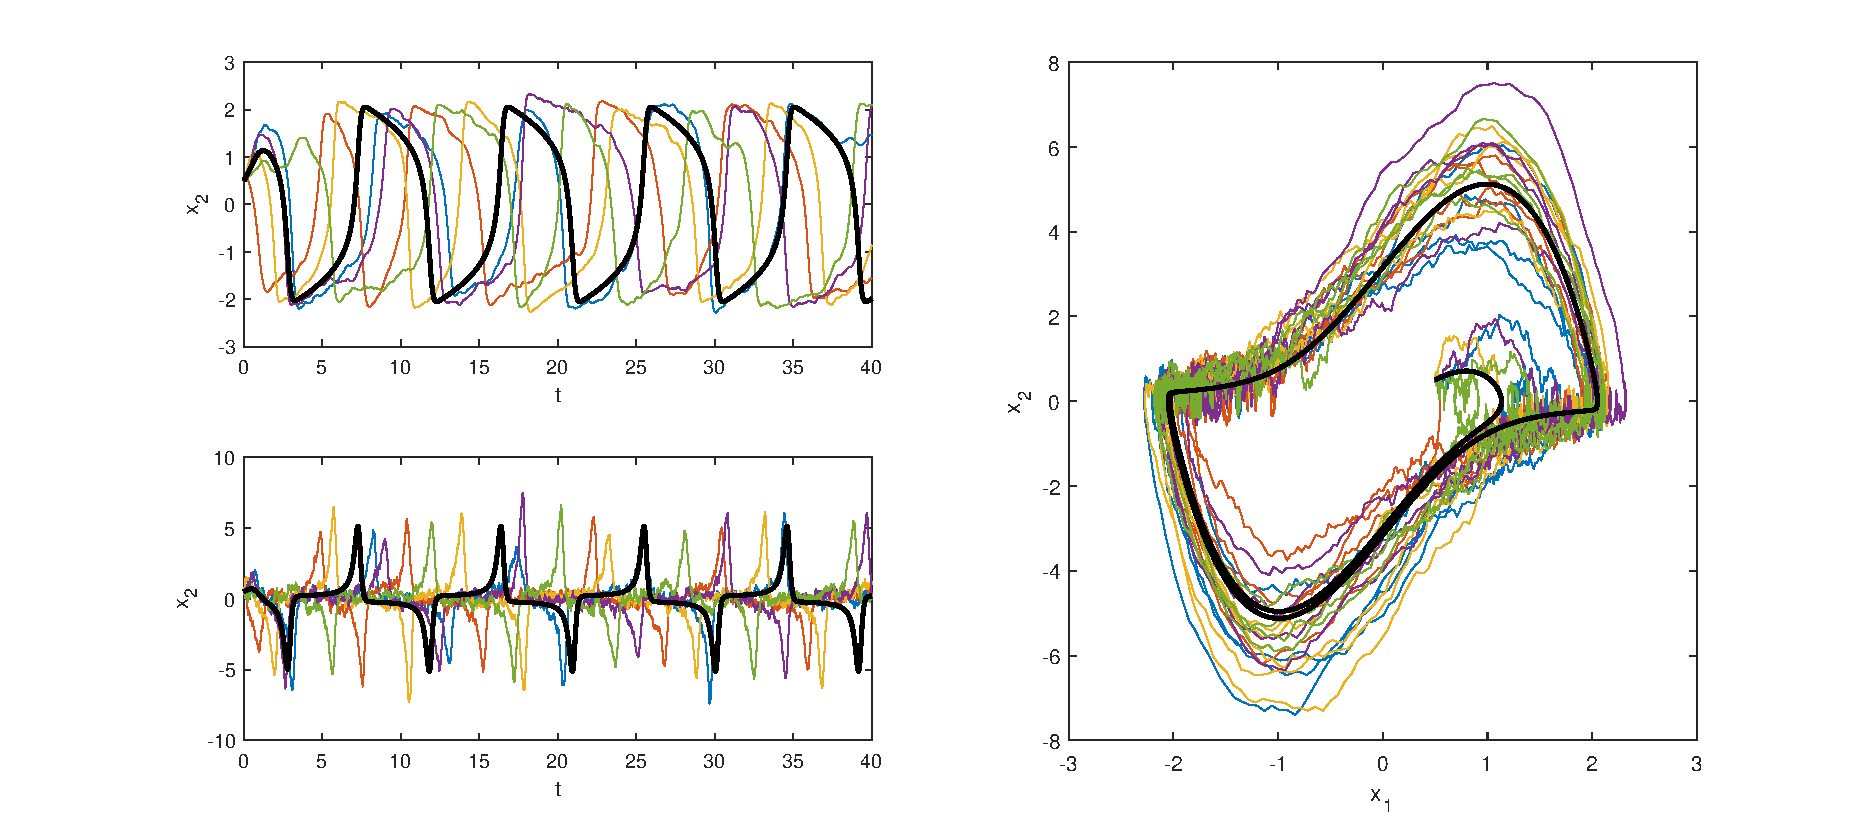
\includegraphics[width=1.25\textwidth]{images/4/4_5_EulerMaruyama_independent.pdf}}
    \caption{5 realisations of the solution for the Van der Pol SDE problem with state independent diffusion ($\mathit{\mu = 3, \sigma=1}$) using Euler-Maruyama with fixed step size}
    \label{4_5_EulerMaruyama_Independent}
\end{figure}

\begin{figure}[H]
    \centering
    \makebox[\textwidth][c]{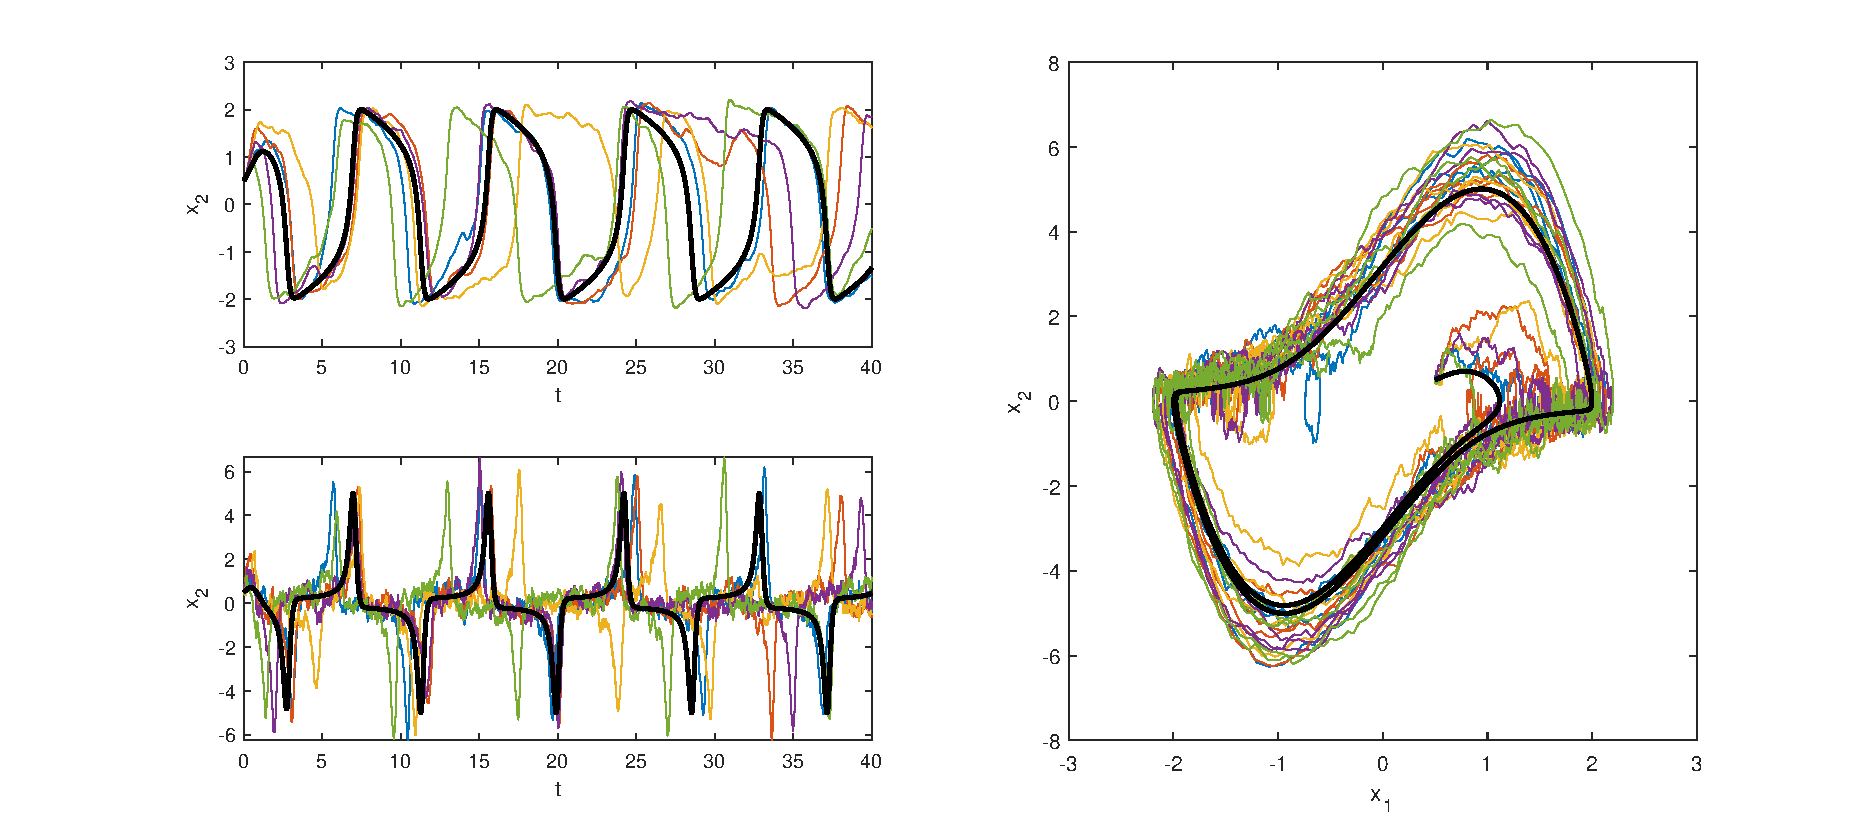
\includegraphics[width=1.25\textwidth]{images/4/4_5_ImplicitExplicit_independent.pdf}}
    \caption{5 realisations of the solution for the Van der Pol SDE problem with state independent diffusion ($\mathit{\mu = 3, \sigma=1}$) using Implicit-Explicit with fixed step size}
    \label{4_5_ImplicitExplicit_Independent}
\end{figure}

\begin{figure}[H]
    \centering
    \makebox[\textwidth][c]{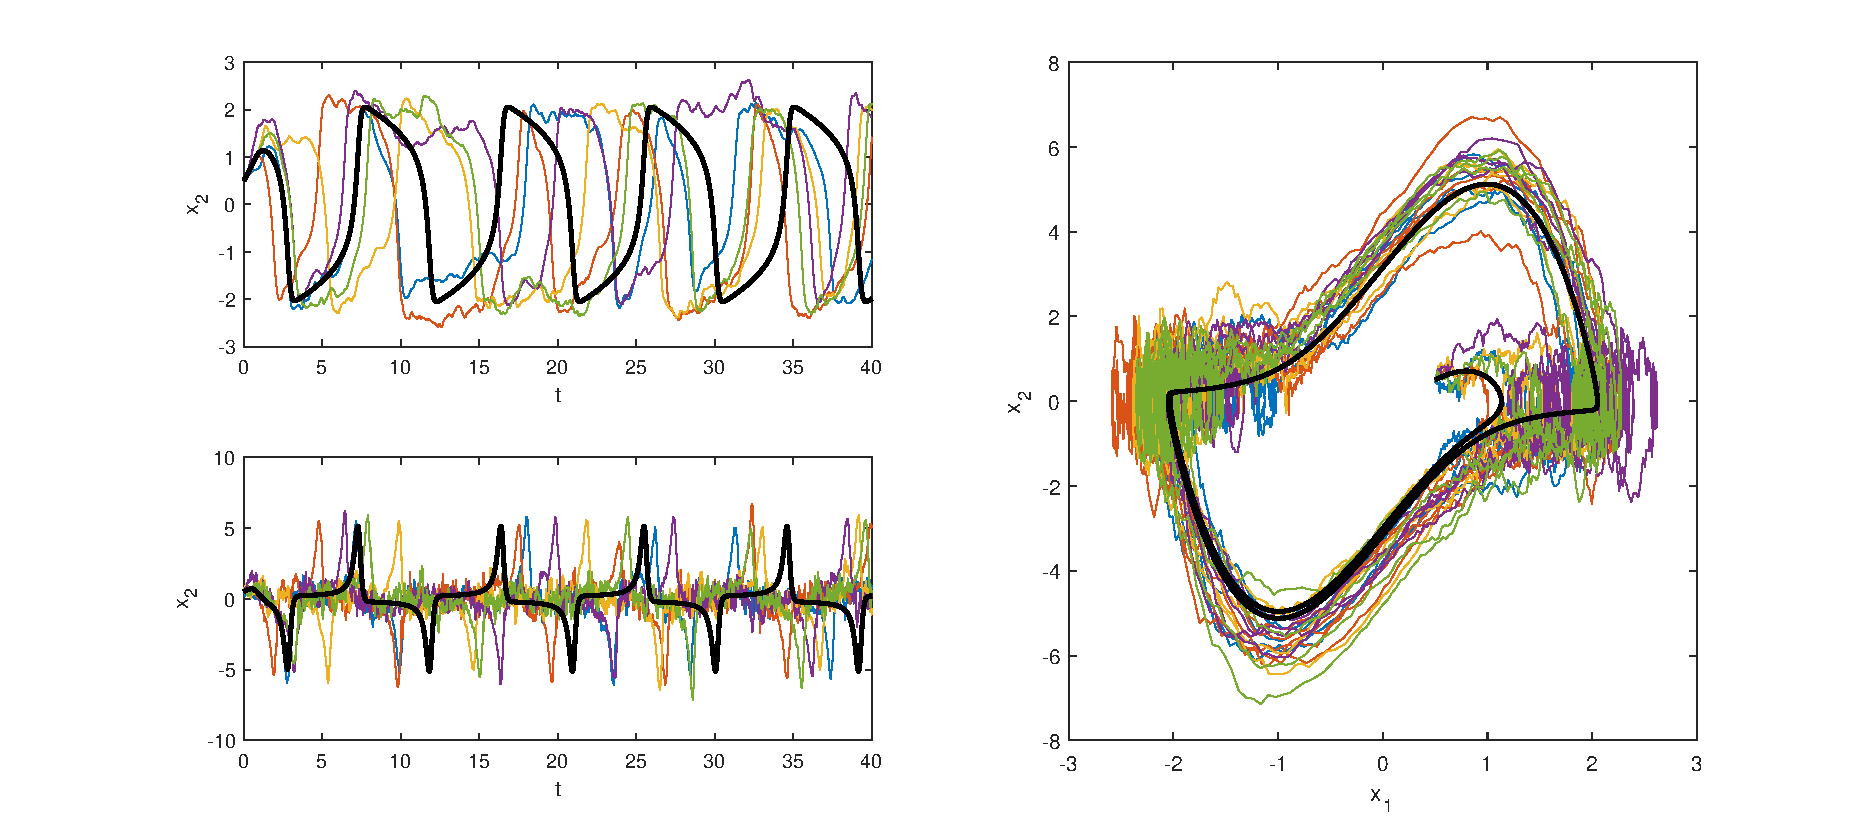
\includegraphics[width=1.25\textwidth]{images/4/4_5_EulerMaruyama_dependent.pdf}}
    \caption{5 realisations of the solution for the Van der Pol SDE problem with state dependent diffusion ($\mathit{\mu = 3, \sigma=0.5}$) using Euler-Maruyama with fixed step size}
    \label{4_5_EulerMaruyama_dependent}
\end{figure}

\begin{figure}[H]
    \centering
    \makebox[\textwidth][c]{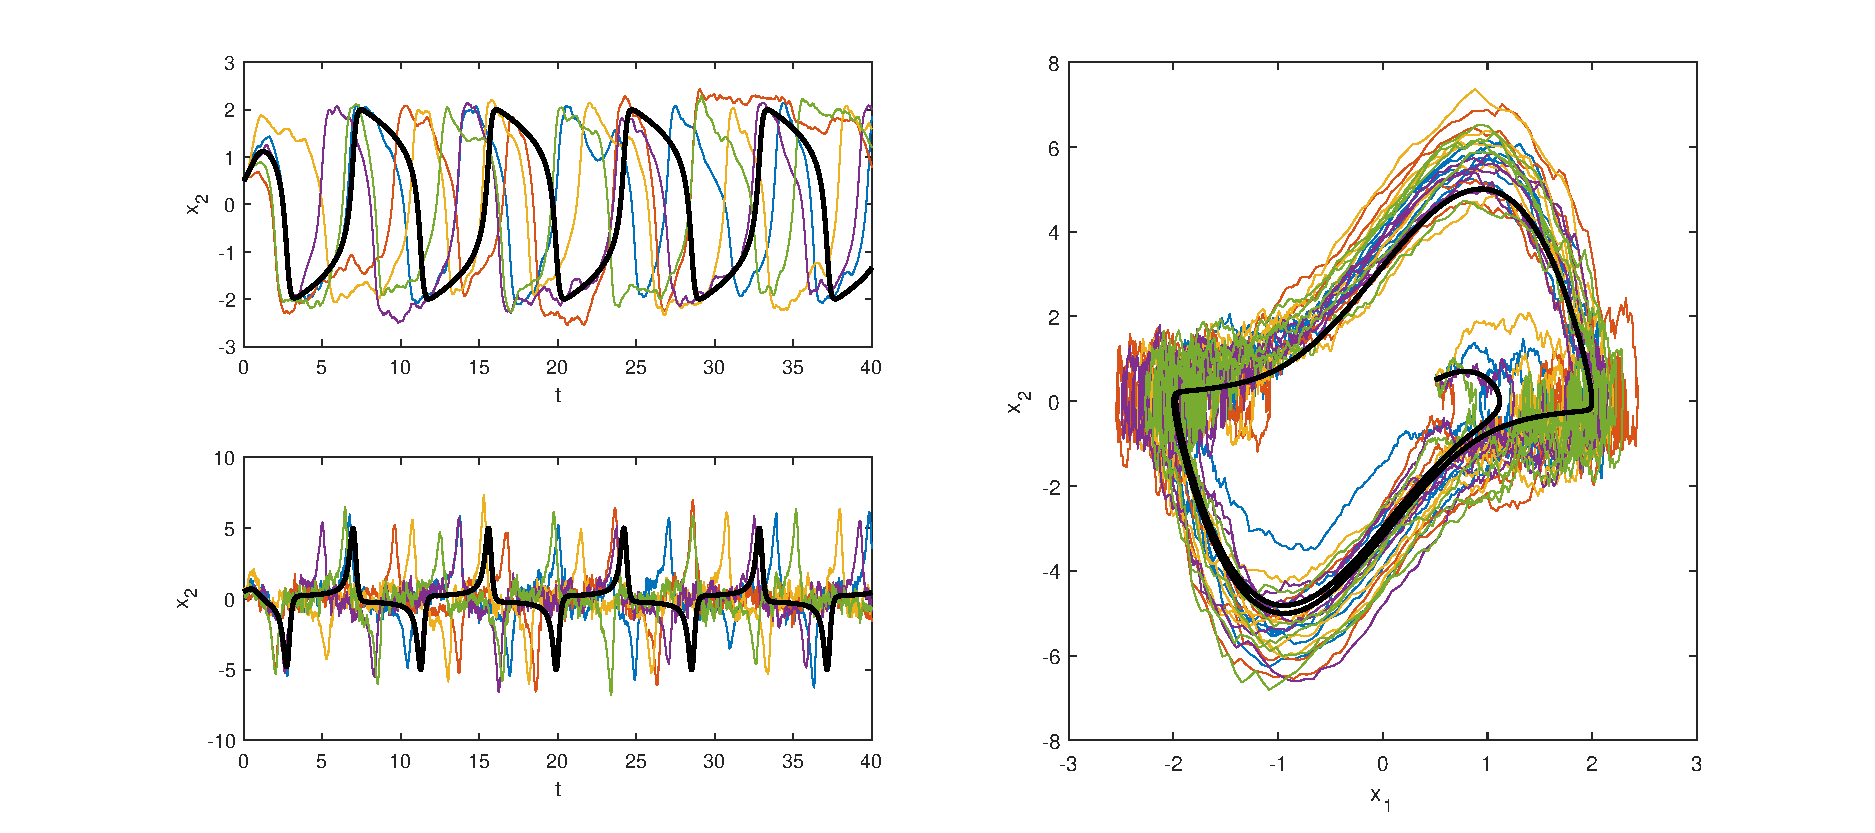
\includegraphics[width=1.25\textwidth]{images/4/4_5_ImplicitExplicit_dependent.pdf}}
    \caption{5 realisations of the solution for the Van der Pol SDE problem with state dependent diffusion ($\mathit{\mu = 3, \sigma=0.5}$) using Implicit-Explicit with fixed step size}
    \label{4_5_ImplicitExplicit_dependent}
\end{figure}

\subsection{Test  your  algorithms  on  the  adiabatic  CSTR  problem  described  in  the papers uploaded to Learn (3D-version and 1D-version).}
For the CSTR problem, we'll also compute 5 realisations of the Euler-Maruyama and the Implicit-Explicit  methods for the 3D and the 1D case. These runs are obtained setting all the parameters as in \cite{Bagterp1} and \cite{Bagterp2}. $\sigma$ was set to $0.5$ for all runs. It's worth noticing how the noise decreases for the 1D problem even though they are run with the same $\sigma$.

\vspace{3cm}

\begin{figure}[H]
\centering
    \begin{subfigure}{0.8\linewidth}
        \centering
        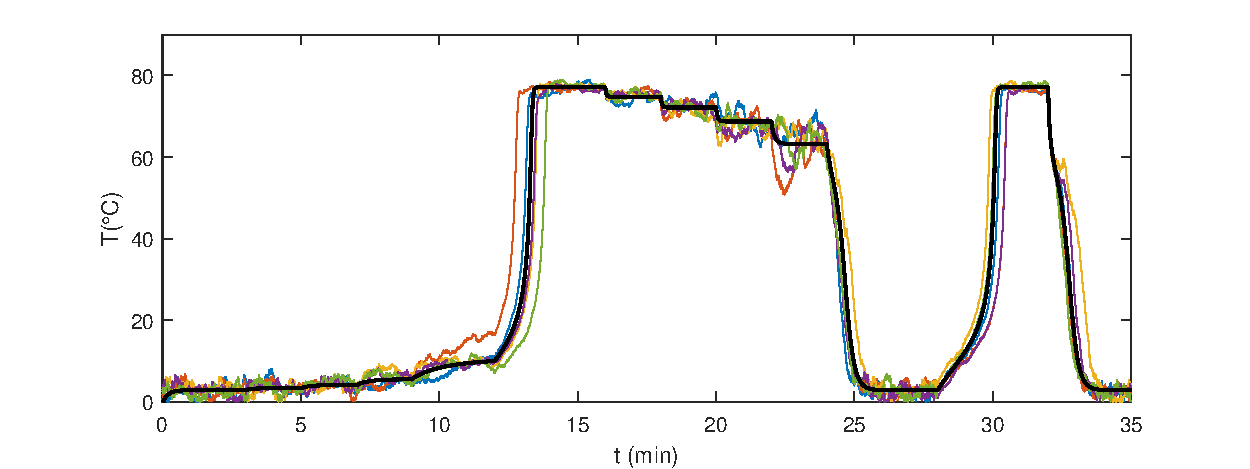
\includegraphics[width=1\linewidth]{images/4/4_6_EulerMaruyama_3D.pdf} 
        \caption{Euler-Maruyama method}
    \end{subfigure} \\
    \begin{subfigure}{0.8\linewidth}
        \centering
        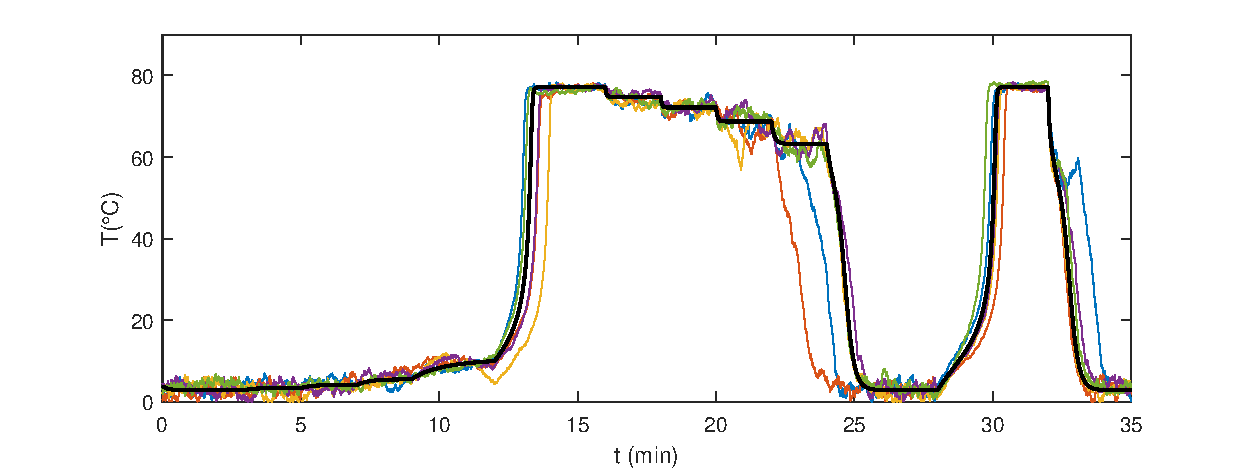
\includegraphics[width=1\linewidth]{images/4/4_6_ImplicitExplicit_3D.pdf}
        \caption{Implicit-Explicit method}
    \end{subfigure}
    \caption{5 realisations of the solution for the 3D CSTR SDE problem ($\sigma = 5$) using fixed step size}
    \label{4_6_EM_vs_IE_3D}
\end{figure}

\vspace{5cm}

\begin{figure}[p]
\centering
    \begin{subfigure}{0.8\linewidth}
        \centering
        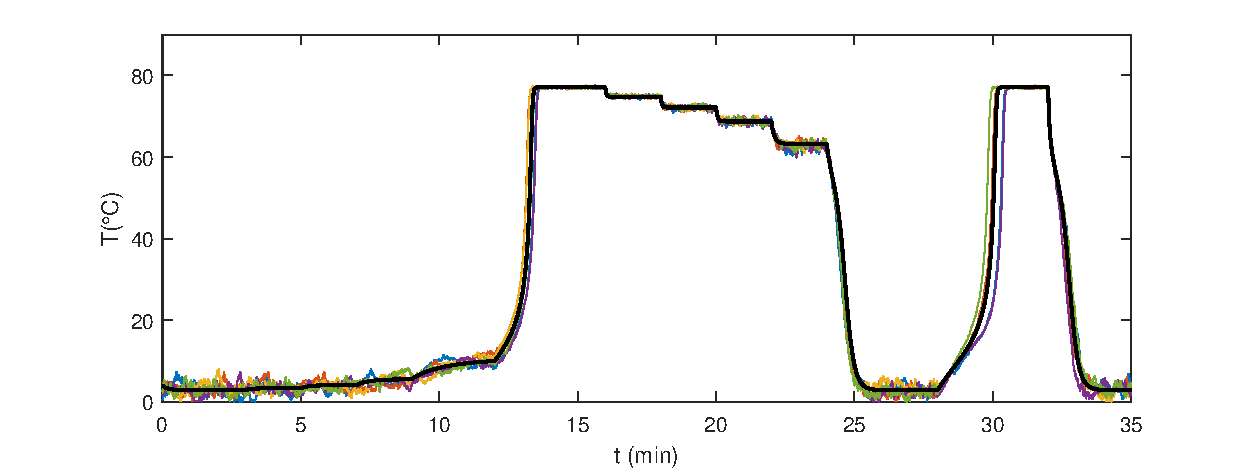
\includegraphics[width=1\linewidth]{images/4/4_6_EulerMaruyama_1D.pdf} 
        \caption{Euler-Maruyama method}
    \end{subfigure} \\
    \begin{subfigure}{0.8\linewidth}
        \centering
        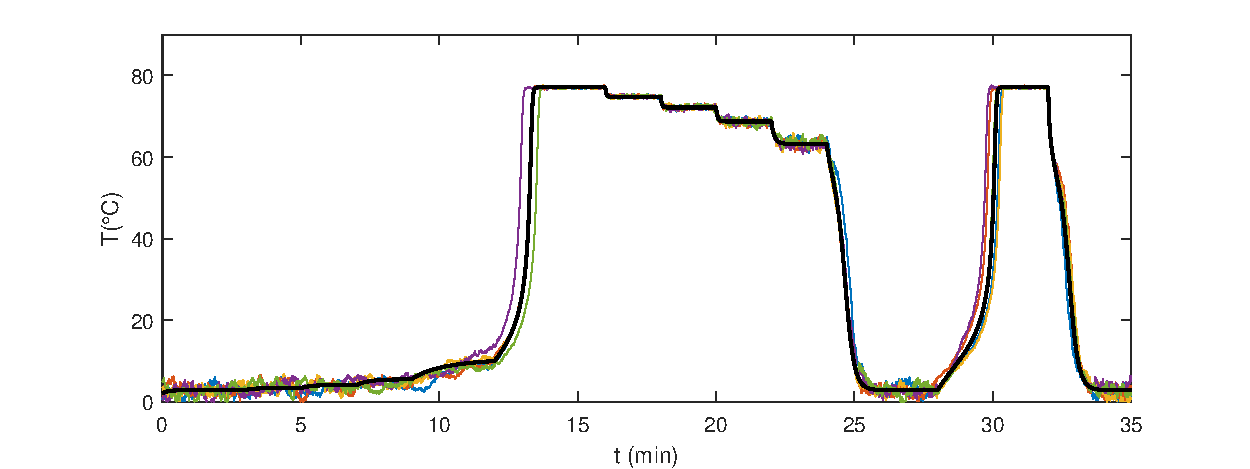
\includegraphics[width=1\linewidth]{images/4/4_6_ImplicitExplicit_1D.pdf}
        \caption{Implicit-Explicit method}
    \end{subfigure}
    \caption{5 realisations of the solution for the 1D CSTR SDE problem ($\sigma = 5$) using fixed step size}
    \label{4_6_EM_vs_IE_1D}
\end{figure}
\pagebreak

\section{Classical Runge-Kutta method with fixed time step size} \label{part5}
We consider again the initial value problem in (\ref{2_problem}).

\subsection{Describe the classical Runge-Kutta method with fixed step size} \label{5_1}

The classical Runge-Kutta is an iterative method used to calculate numerical approximations to the solution of initial value problems. It works by taking a time step size $h$, where we will perform the following calculations:

\begin{align*}
    &T_1 = t_n &&X_1 = x_n \\
    &T_2 = t_n + \frac{1}{2}h  &&X_2 = x_n + h\frac{1}{2}f(T_1, X_1) \\
    &T_3 = t_n + \frac{1}{2}h  &&X_3 = x_n + h\frac{1}{2}f(T_2, X_2) \\
    &T_4 = t_n + h  &&X_4 = x_n + hf(T_3, X_3) \\
\end{align*}
Once this is calculated, we can get the actual step that we will store as part of our solution as follows:
\begin{gather*}
    t_{n+1} = t_n + h \\
    x_{n+1} = x_n + h\left(\frac{1}{6}f(T_1, X_1) + \frac{1}{3}f(T_2,X_2) + \frac{1}{3}f(T_3, X_3) + \frac{1}{6}f(T_4,X_4)\right)
\end{gather*}
Note that the previous 8 calculations must be performed in every single step. To solve the initial value problem we just start from $x_0$, pick a step size $h$, and iterate over the algorithm.

\begin{table}[H]
    \centering
    \begin{tabular}{c|cccc}
    0   &     &     &     &     \\
    $\nicefrac{1}{2}$ & $\nicefrac{1}{2}$ &     &     &     \\
    $\nicefrac{1}{2}$ & 0   & $\nicefrac{1}{2}$ &     &     \\
    $1$   & 0   & 0   & $1$   &     \\ \hline
    x   & $\nicefrac{1}{6}$ & $\nicefrac{1}{3}$ & $\nicefrac{1}{3}$ & $\nicefrac{1}{6}$
    \end{tabular}
    \caption{Butcher Tableau of the classical Runge-Kutta method}
    \label{5_BT_RK4}
\end{table}

%%%%%%%%%%%%%%%%%%%%%%%%%%%%%%%%%%%%%%%%%%%%%%%%%%%%%%%%%%%%%%%%%%%%%%%%%%%%%%%%%%%%%%%%%%%%%%%%%%%

\subsection{Implement an algorithm in Matlab for the classical Runge-Kutta method with fixed time step size. Provide the code in your report.  Use a format that enables syntax highlighting. Comment on the code}
We implement the classical Runge-Kutta method with fixed time step size with the following code:
\begin{lstlisting}[caption = Classical Runge-Kutta method with fixed time step size, captionpos=b, label=1_ClassicRK4]
function [T, X] = ClassicRK4_fixed(fun,tspan,h,x0,args)
% time interval
t0 = tspan(1);
tf = tspan(end);
T = t0:h:tf;
N = size(T,2);
X = zeros(size(x0,1), N);
X(:,1) = x0;

for k = 1:N-1
    t = T(k);
    x = X(:,k);

    % Stage 1
    T1 = t;
    X1 = x;
    F1 = feval(fun,T1,X1,args{:});
    % Stage 2
    T2 = t + h/2;
    X2 = x + h/2*F1;
    F2 = feval(fun,T2,X2,args{:});
    % Stage 3
    T3 = T2;
    X3 = x + h/2*F2;
    F3 = feval(fun,T3,X3,args{:});
    % Stage 4
    T4 = t + h;
    X4 = x + h*F3;
    F4 = feval(fun,T4,X4,args{:});

    % final solution
    X(:,k+1) = x + h*(1/6*F1+1/3*F2+1/3*F3+1/6*F4);

end
end
\end{lstlisting}

This implementation uses the following input arguments:
\begin{itemize}
    \item \code{fun} is a pointer to a function where our IVP function $f$ is defined.
    \item \code{tspan} is a vector of two values stating the initial and final time of the simulation.
    \item \code{x0} is the initial condition, i.e. the value of $x(t_0)$.
    \item \code{h} is the fixed time step size we want for our simulation.
    \item \code{args} is an array that includes constants needed to calculate the IVP function ($\mu$ in the Van der Pol problem, $\lambda$ in the test equation, all the parameters in the CSTR problem).
\end{itemize}


%%%%%%%%%%%%%%%%%%%%%%%%%%%%%%%%%%%%%%%%%%%%%%%%%%%%%%%%%%%%%%%%%%%%%%%%%%%%%%%%%%%%%%%%%%%%%%%%%%%
\subsection{Test your problem for test equation. Discuss order and stability of the numerical method} \label{5_3}
We will proceed testing the classical Runge-Kutta method (RK4) in a similar manner as we did for the Explicit and Implicit Euler methods in part \ref{part1}. As the RK4 has order 4, we should observe the local error having order 5 and the global error having order 4. Results are shown in the folowing figures, setting $\lambda=-1$, $h=0.2$ for \ref{5_3_TE} and $\code{tspan}=[0, 30]$ for \ref{5_3_TE_errors}.

The shape of the local and global errors vs. time is very similar to the one obtained for the Explicit and Implicit Euler in Figure \ref{1_3_errors}. However, both having the same time step size, the solution of the RK4 is a lot more precise. The scale of the errors is not even comparable.

\begin{figure}[H]
    \centering
    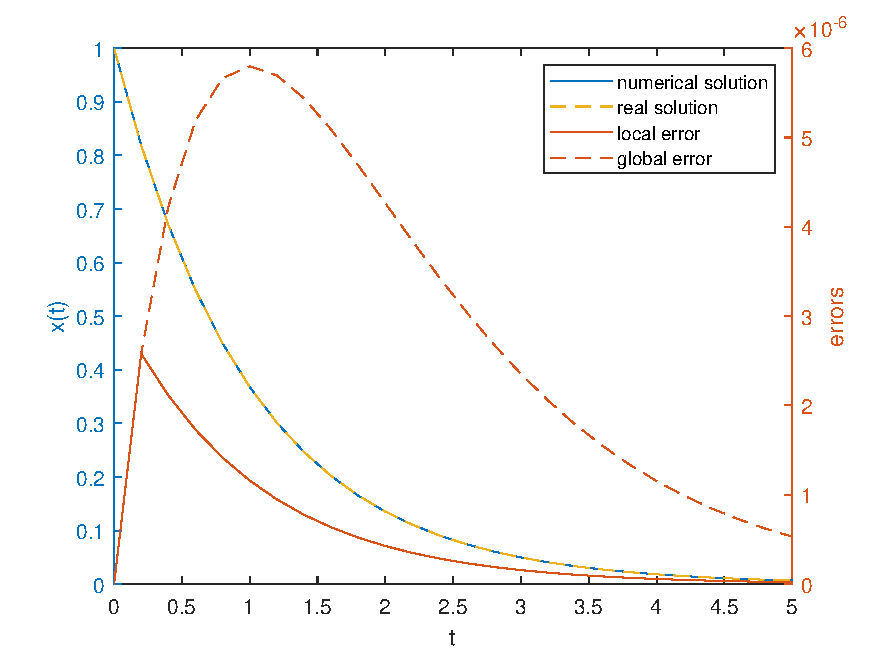
\includegraphics[width=0.7\linewidth]{images/5/5_3_TestEquation.pdf} 
    \caption{Solution and errors vs. time for the Test equation using fixed classical Runge-Kutta method}
    \label{5_3_TE}
\end{figure}

\begin{figure}[H]
\centering
    \begin{subfigure}{0.49\linewidth}
        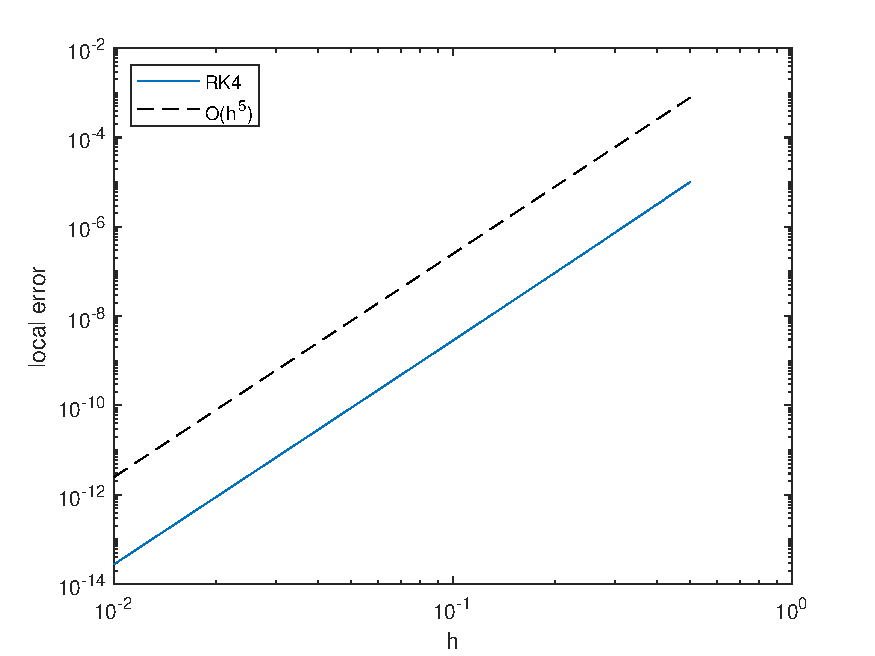
\includegraphics[width=\linewidth]{images/5/5_3_localerror.pdf}
        \caption{Local error}
    \end{subfigure}
    \begin{subfigure}{0.49\linewidth}
        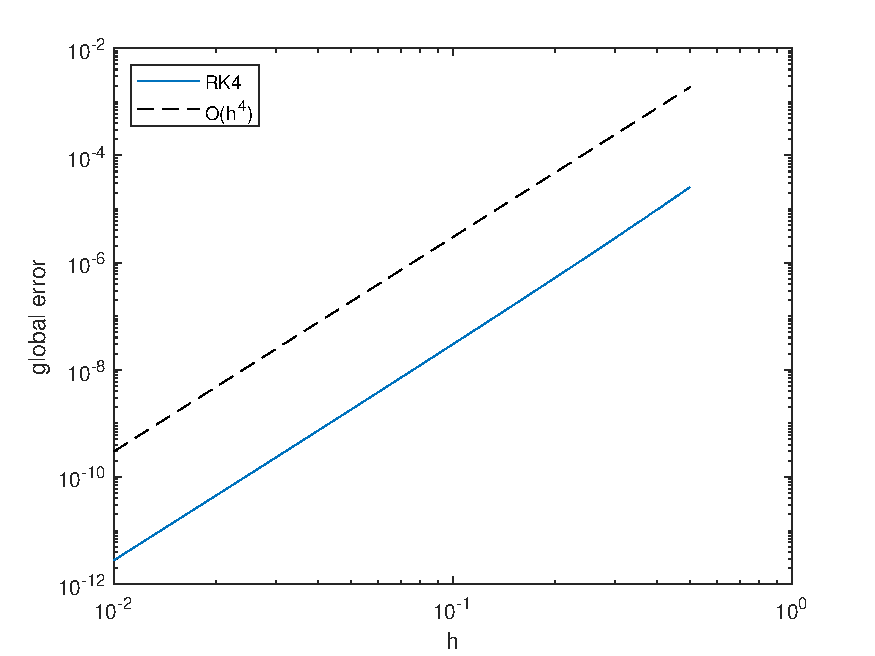
\includegraphics[width=\linewidth]{images/5/5_3_globalerror.pdf}
        \caption{Global error}
    \end{subfigure}
    \caption{Local and global errors vs. time-step size for the Test equation using fixed classical Runge-Kutta method}
    \label{5_3_TE_errors}
\end{figure}

For the stability of the method, the solution by a Runge-Kutta method for the test equation is given as:
\begin{equation} \label{stability_region_formula}
    x_{n+1} = R(h \lambda) x_n \hspace{1em} R(z) = 1 + z b'(I-zA)^(-1)e,
\end{equation}
where, A and b are the top right matrix and the bottom right vector in the Butcher Tableau \ref{5_BT_RK4}. The stability regions for complex values of $h\lambda$ are shown in Figure \ref{5_3_stability_regions}. Here we can observe that the method is neither A-stable, nor L-stable, given that there are regions on the left side plane that are greater than 1 and that $\lim_{z \to -\infty}|R(z)| \neq 0$.

\begin{figure}[H]
    \centering
    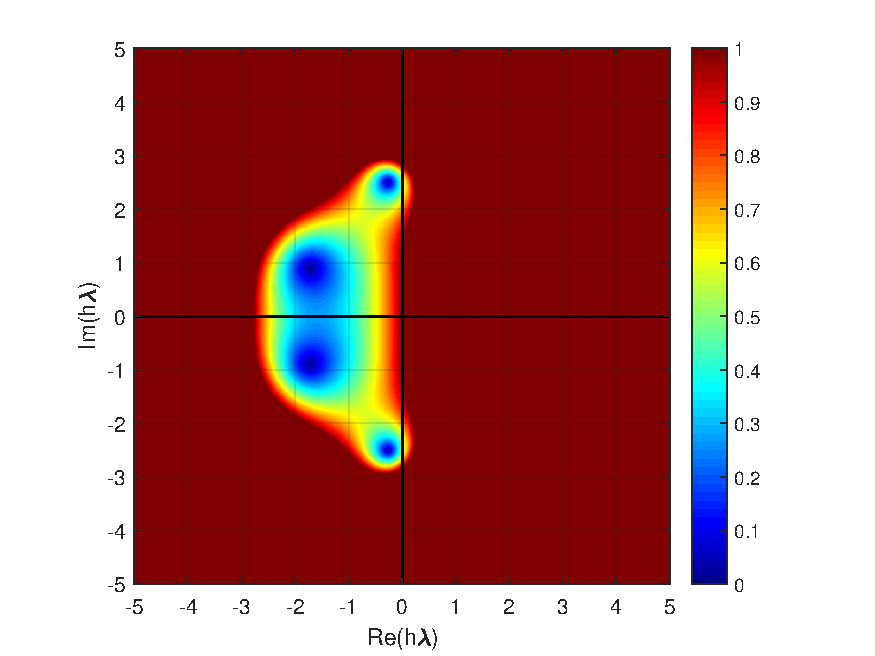
\includegraphics[width=0.7\linewidth]{images/5/5_3_stability_regions.pdf} 
    \caption{Values of $R(h\lambda)$ for the classical Runge-Kutta method}
    \label{5_3_stability_regions}
\end{figure}

%%%%%%%%%%%%%%%%%%%%%%%%%%%%%%%%%%%%%%%%%%%%%%%%%%%%%%%%%%%%%%%%%%%%%%%%%%%%%%%%%%%%%%%%%%%%%%%%%%%

\subsection{Test your algorithms on the Van der Pol problem \texorpdfstring{($\mathbf{\mu = 1.5}$ and $\mathbf{\mu = 15}$, $\mathbf{x_0 = [1.0;1.0]}$).}{(mu = 1.5 and mu = 15, x0 = [1.0;1.0]).}}
We can observe that the classical Runge-Kutta manages to approach the real solution with a way bigger step size than the Explicit Euler (Figures \ref{2_4_fixed_mu_1_5} and \ref{2_4_fixed_mu_15}) in both cases. However, for $\mu=15$ we need to lower the step size almost by a factor of 10 due to the larger stiffness of the problem. After all, the classical Runge-Kutta is a explicit method and thus suffer from the same problems as the Explicit Euler.

\begin{figure}[H]
    \centering
    \makebox[\textwidth][c]{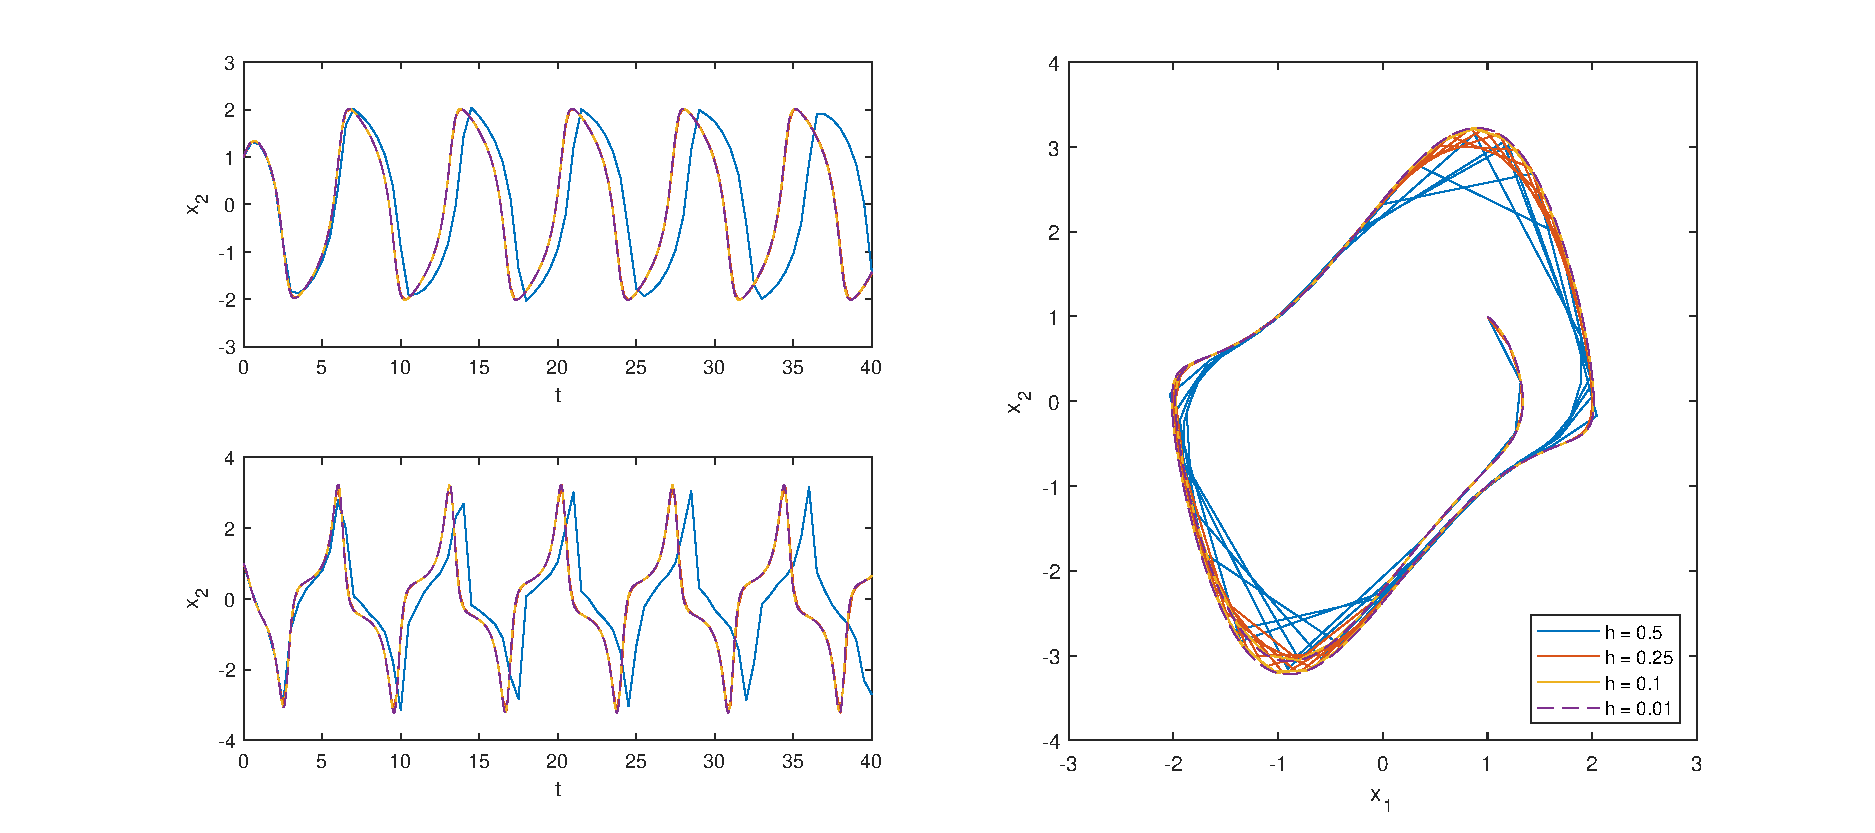
\includegraphics[width=1.25\textwidth]{images/5/5_4_RK4_mu_1_5.pdf}}
    \caption{Solution for the Van der Pol problem ($\mathit{\mu = 1.5}$) using classical Runge-Kutta with fixed step size}
    \label{5_4_RK4_mu_1_5}
\end{figure}

\begin{figure}[H]
    \centering
    \makebox[\textwidth][c]{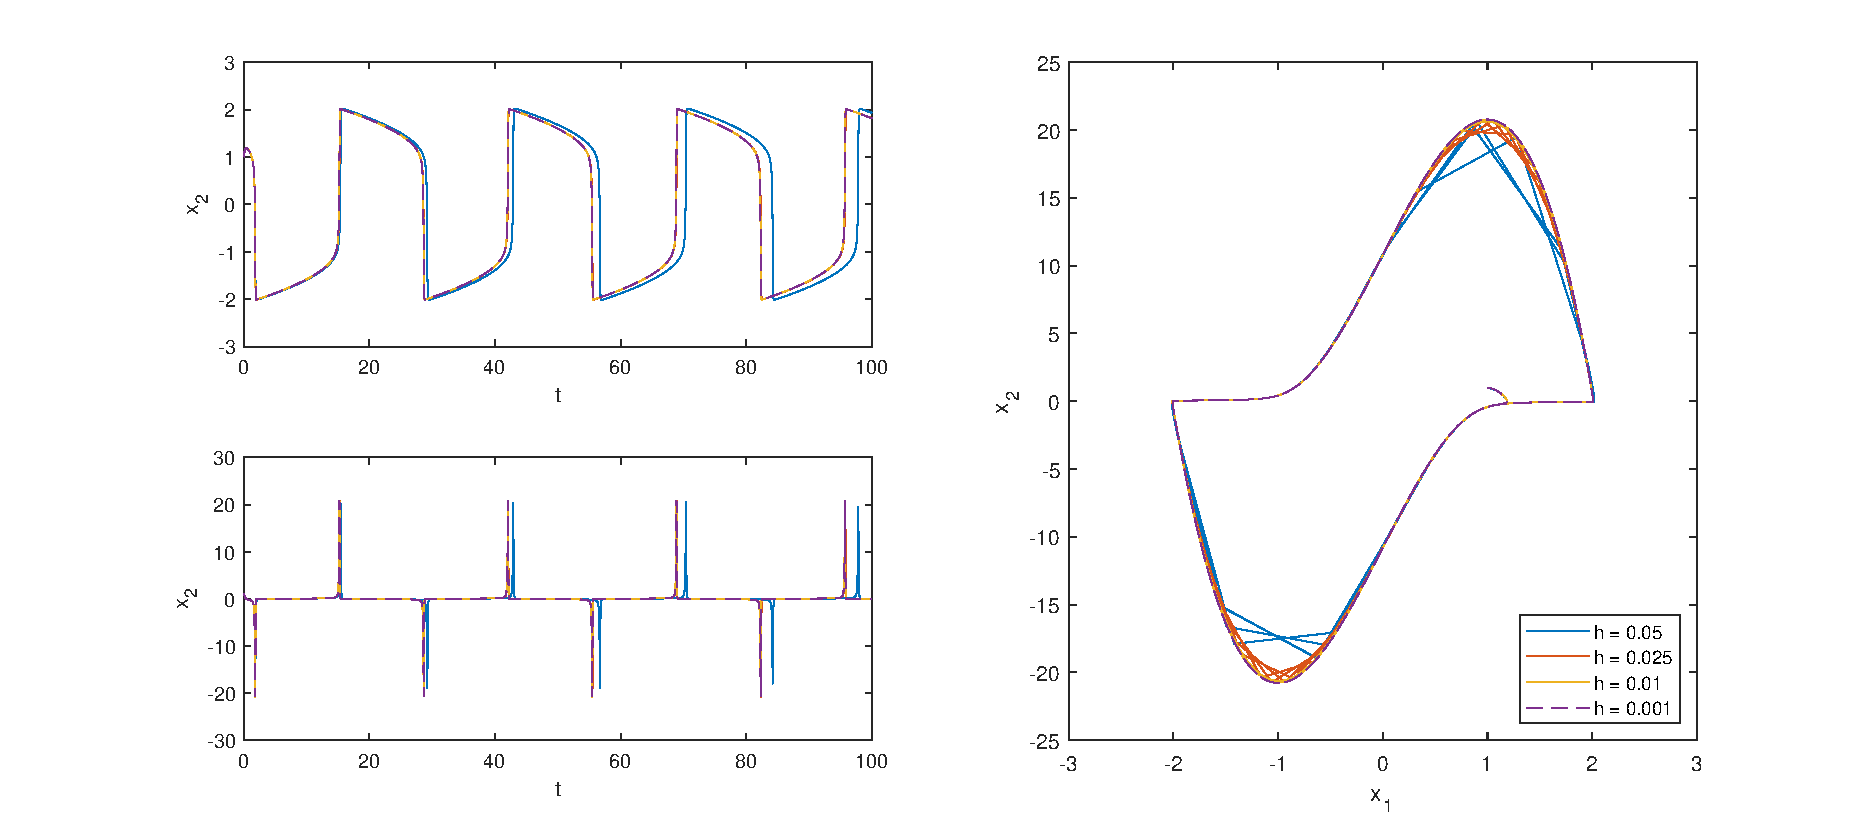
\includegraphics[width=1.25\textwidth]{images/5/5_4_RK4_mu_15.pdf}}
    \caption{Solution for the Van der Pol problem ($\mathit{\mu = 15}$) using classical Runge-Kutta with fixed step size}
    \label{5_4_RK4_mu_15}
\end{figure}


%%%%%%%%%%%%%%%%%%%%%%%%%%%%%%%%%%%%%%%%%%%%%%%%%%%%%%%%%%%%%%%%%%%%%%%%%%%%%%%%%%%%%%%%%%%%%%%%%%%

\subsection{Test  your  algorithms  on  the  adiabatic  CSTR  problem  described  in  the
papers uploaded to Learn (3D-version and 1D-version).}
For the CSTR problem, we can still see an increase in performance compared to the Explicit Euler (Figure \ref{2_5_3D_1D_hs}) but not as significant as in the Van der Pol case. We can still see the spiky behaviour when $T$ reaches its maximum (low $F$), when the problem is more stiff. The step size of $h=0.1$ already approaches the solution pretty good, only failing at some values in this stiff area of the problem.
\begin{figure}[H]
\centering
    \begin{subfigure}{0.8\linewidth}
        \centering
        \includegraphics[width=1\linewidth]{images/5/5_5_CSTR_3D.pdf} 
        \caption{CSTR 3D problem}
    \end{subfigure} \\
    \begin{subfigure}{0.8\linewidth}
        \centering
        \includegraphics[width=1\linewidth]{images/5/5_5_CSTR_1D.pdf}
        \caption{CSTR 1D problem}
    \end{subfigure}
    \caption{Solution for the CSTR problem using classical Runge-Kutta with fixed step size}
    \label{5_5_3D_1D}
\end{figure}

\subsection{Compare the results from your algorithms with the results you get using some of Matlab's ODE solvers}
As in this part the classical Runge-Kutta with fixed time step size has been the only one implemented, we cannot directly compare to the chosen Matlab solvers (\code{ode45} and \code{ode15s}), as they both use adaptive step size. We'll compare the classical Runge-Kutta in next section, Exercise \ref{6_6}, with its adaptive version.

\pagebreak

\section{Classical Runge-Kutta method with adaptive time step}
We consider again the initial value problem in (\ref{2_problem}).
\subsection{Describe the classical Runge-Kutta method with adaptive step size}
The classical Runge-Kutta is described in exercise \ref{5_1}. The only change introduced in this part will be implementing the error estimation using step doubling and the asymptotic step size controller.

%%%%%%%%%%%%%%%%%%%%%%%%%%%%%%%%%%%%%%%%%%%%%%%%%%%%%%%%%%%%%%%%%%%%%%%%%%%%%%%%%%%%%%%%%%%%%%%%%%%
\subsection{Implement an algorithm in Matlab for the classical Runge-Kutta method with adaptive time step size. Provide the code in your report.  Use a format that enables syntax highlighting. Comment on the code}
\begin{lstlisting}[caption = Classical Runge-Kutta method with adaptive time step size, captionpos=b, label=6_ClassicRK4_adaptive]
function [T,X,r_out,h_out,info] = ClassicRK4_adaptive(fun,tspan,h0,x0,abstol,reltol,args)

epstol = 0.8;
kpow = 0.2;
facmin = 0.1;
facmax = 5.0;

t0 = tspan(1);
tf = tspan(end);
t = t0;
h = h0;
x = x0;

T = t0;
X = x0;
r_out = [];
h_out = [];
info = zeros(1,4);

nfun = 0;
nstep = 0;
naccept = 0;

while t < tf
    if (t+h > tf)
        h = tf-t;
    end
    
    nfun = nfun + 1;
    AcceptStep = false;
    while ~AcceptStep
        x1 = ClassicRK4_step(fun,t,h,x,args);
        nfun = nfun + 4;
        
        hm = 0.5*h;
        tm = t + hm;
        xm = ClassicRK4_step(fun,t,hm,x,args);
        nfun = nfun + 4;
        x1hat = ClassicRK4_step(fun,tm,hm,xm,args);
        nfun = nfun + 4;
        nstep = nstep + 1;
        
        e = abs(x1hat-x1);
        r = max(e./max(abstol, abs(x1hat) .* reltol));
        AcceptStep = (r <= 1.0);
        
        if AcceptStep
            t = t+h;
            x = x1hat;
            
            T = [T,t];
            X = [X,x];
            r_out = [r_out, r];
            h_out = [h_out, h];
            naccept = naccept + 1;
        end
        
        h = max(facmin, min((epstol/r)^kpow, facmax)) * h;
    end
end

info(1) = nfun;
info(2) = nstep;
info(3) = naccept;
info(4) = nstep - naccept;

end
\end{lstlisting}

%%%%%%%%%%%%%%%%%%%%%%%%%%%%%%%%%%%%%%%%%%%%%%%%%%%%%%%%%%%%%%%%%%%%%%%%%%%%%%%%%%%%%%%%%%%%%%%%%%%
\subsection{Test your problem for test equation. Discuss order and stability of the numerical method}
Implementing the adaptive classical Runge-Kutta just as we did for the classical one leads us to the results shown below. It's curious to see that the relation between the local and global error vs. the tolerance. The relation between them was found empirically.

The stability of the method is already discussed in Exercise \ref{5_3}.

\begin{figure}[H]
    \centering
    \includegraphics[width=0.7\linewidth]{images/6/6_3_TestEquation.pdf} 
    \caption{Solution and errors vs. time for the Test equation using adaptive classical Runge-Kutta method}
    \label{6_3_TE}
\end{figure}

\begin{figure}[H]
\centering
    \begin{subfigure}{0.49\linewidth}
        \includegraphics[width=\linewidth]{images/6/6_3_localerror.pdf}
        \caption{Local error}
    \end{subfigure}
    \begin{subfigure}{0.49\linewidth}
        \includegraphics[width=\linewidth]{images/6/6_3_globalerror.pdf}
        \caption{Global error}
    \end{subfigure}
    \caption{Local and global errors vs. time-step size for the Test equation using adaptive classical Runge-Kutta method}
    \label{6_3_TE_errors}
\end{figure}

%%%%%%%%%%%%%%%%%%%%%%%%%%%%%%%%%%%%%%%%%%%%%%%%%%%%%%%%%%%%%%%%%%%%%%%%%%%%%%%%%%%%%%%%%%%%%%%%%%%
\subsection{Test your algorithms on the Van der Pol problem \texorpdfstring{($\mathbf{\mu = 1.5}$ and $\mathbf{\mu = 15}$, $\mathbf{x_0 = [1.0;1.0]}$).}{(mu = 1.5 and mu = 15, x0 = [1.0;1.0]).}}
The results for the Van der pol problem are shown below. When comparing to the Explicit Euler with adaptive results shown in Figures \ref{2_4_adaptive_mu_1_5} and \ref{2_4_adaptive_mu_15}, we can see that the method achieves better performance when working with same tolerances, or even larger. The change of frequency of the signals has disappeared completely and all tolerances approach the real solution pretty good. However, as it's an explicit method, it's still sensible to the stiffness of the Van der Pol with $\mu=15$. Specially, comparing Tables \ref{2_4_adaptive_mu_15_table} and \ref{6_4_adaptive_mu_15_table}, we can see how the number of necessary steps is a lot smaller in the Runge-Kutta. However, for smaller tolerances the number of function evaluations is higher. Thus, the Runge-Kutta method is a better alternative if we are interested in a very precise solution, with a very low tolerance.

\begin{figure}[H]
    \centering
    \makebox[\textwidth][c]{\includegraphics[width=1.25\textwidth]{images/6/6_4_adaptive_mu_1_5.pdf}}
    \caption{Solution for the Van der Pol problem ($\mathit{\mu = 1.5}$) using classical Runge-Kutta with adaptive step size}
    \label{6_4_RK4_mu_1_5}
\end{figure}

\begin{table}[H]
    \centering
    \begin{tabular}{@{}l|cccc@{}}
    \toprule
    Tolerances           & 0.5  & 0.05 & 0.001 & 1e-05 \\ \midrule
    Function evaluations & 1335 & 1690 & 2843  & 6440  \\
    Calculated steps     & 106  & 134  & 224   & 506   \\
    Accepted steps       & 63   & 82   & 155   & 368   \\
    Rejected steps       & 43   & 52   & 69    & 138   \\ \bottomrule
    \end{tabular}
    \caption{Parameters of the classical Runge-Kutta with adaptive step size for the Van der Pol problem ($\mathit{\mu = 1.5}$)}
    \label{6_4_adaptive_mu_1_5_table}
\end{table}

\begin{figure}[H]
    \centering
    \makebox[\textwidth][c]{\includegraphics[width=1.25\textwidth]{images/6/6_4_adaptive_mu_15.pdf}}
    \caption{Solution for the Van der Pol problem ($\mathit{\mu = 15}$) using classical Runge-Kutta with adaptive step size}
    \label{6_4_RK4_mu_15}
\end{figure}

\begin{table}[H]
    \centering
    \begin{tabular}{@{}l|cccc@{}}
    \toprule
    Tolerances           & 0.05  & 0.005 & 0.0001 & 1e-06 \\ \midrule
    Function evaluations & 10951 & 11526 & 14814  & 26382 \\
    Calculated steps     & 867   & 910   & 1164   & 2050  \\
    Accepted steps       & 547   & 606   & 846    & 1782  \\
    Rejected steps       & 320   & 304   & 318    & 268   \\ \bottomrule
    \end{tabular}
    \caption{Parameters of the classical Runge-Kutta with adaptive step size for the Van der Pol problem ($\mathit{\mu = 15}$)}
    \label{6_4_adaptive_mu_15_table}
\end{table}

\pagebreak

%%%%%%%%%%%%%%%%%%%%%%%%%%%%%%%%%%%%%%%%%%%%%%%%%%%%%%%%%%%%%%%%%%%%%%%%%%%%%%%%%%%%%%%%%%%%%%%%%%%
\subsection{Test  your  algorithms  on  the  adiabatic  CSTR  problem  described  in  the papers uploaded to Learn (3D-version and 1D-version).}
Just as in the Van der Pol, the classical Runge-Kutta with adaptive step size manages to outperform the convergence achieved by the Explicit Euler. It also deals a lot better with the stiff area of the problem. However, even though it needs less steps to achieve a better solution with the same tolerance, the extra amount of function evaluations per step makes it only worthed when the tolerance is pretty small.

\begin{figure}[H]
    \centering
    \makebox[\textwidth][c]{\includegraphics[width=1\textwidth]{images/6/6_5_3D_tols.pdf}}
    \caption{Solution for the CSTR 3D problem using classical Runge-Kutta with adaptive step size}
    \label{6_5_3D_tols}
\end{figure}

\begin{table}[H]
    \centering
    \begin{tabular}{@{}l|cccc@{}}
    \toprule
    Tolerances           & 0.02 & 0.005 & 0.001 & 1e-05 \\ \midrule
    Function evaluations & 2068 & 2168  & 2650  & 4274  \\
    Calculated steps     & 163  & 170   & 208   & 334   \\
    Accepted steps       & 112  & 128   & 154   & 266   \\
    Rejected steps       & 51   & 42    & 54    & 68    \\ \bottomrule
    \end{tabular}
    \caption{Parameters of the classical Runge-Kutta with adaptive step size for the CSTR 3D problem}
    \label{6_5_3D_tols_table}
\end{table}

\begin{figure}[H]
    \centering
    \makebox[\textwidth][c]{\includegraphics[width=1\textwidth]{images/6/6_5_1D_tols.pdf}}
    \caption{Solution for the CSTR 1D problem using classical Runge-Kutta with adaptive step size}
    \label{6_5_1D_tols}
\end{figure}

\begin{table}[H]
    \centering
    \begin{tabular}{@{}l|cccc@{}}
    \toprule
    Tolerances           & 0.02 & 0.005 & 0.001 & 1e-05 \\ \midrule
    Function evaluations & 1741 & 1909  & 2143  & 3425  \\
    Calculated steps     & 137  & 150   & 168   & 268   \\
    Accepted steps       & 97   & 109   & 127   & 209   \\
    Rejected steps       & 40   & 41    & 41    & 59    \\ \bottomrule
    \end{tabular}
    \caption{Parameters of the classical Runge-Kutta with adaptive step size for the CSTR 1D problem}
    \label{6_5_1D_tols_table}
\end{table}


%%%%%%%%%%%%%%%%%%%%%%%%%%%%%%%%%%%%%%%%%%%%%%%%%%%%%%%%%%%%%%%%%%%%%%%%%%%%%%%%%%%%%%%%%%%%%%%%%%%
\subsection{Compare the results from your algorithms with the results you get using some of Matlab's ODE solvers} \label{6_6}
For the Van der Pol problem, we tested the classical Runge-Kutta against \code{ode45} for the non-stiff case ($\mu = 1.5$), and against \code{ode15s} for the stiff case ($\mu = 15$). With this method, we are already approaching the ``big leagues" of ODE solvers. We can observe directly the effect that having a greater order of the error has on the solution: it's a lot more precise with big tolerances. Actually, the classical Runge-Kutta achieves similar accuracy to the \code{ode45}, when not better. However, this all comes with a cost, the number of function evaluations is also larger, but it's not as far from it as both Euler methods. As it's an explicit method, it doesn't stand a chance against the \code{ode15s} in the stiff case when looking at the number of function evaluations. However, the accuracy of the method is still surprisingly good, specially for low tolerances, where the \code{ode15s} misses the solution.

\begin{figure}[H]
    \centering
    \makebox[\textwidth][c]{\includegraphics[width=1.25\textwidth]{images/6/6_6_mu_1_5.pdf}}
    \caption{Solution for the Van der Pol problem ($\mathit{\mu = 1.5}$) using Classical Runge-Kutta vs. \code{ode45}}
    \label{6_6_mu_1_5}
\end{figure}

\begin{table}[H]
    \centering
    \begin{tabular}{@{}l|cc|cc@{}}
    \toprule
    \textbf{Method}      & \multicolumn{2}{c|}{\textbf{RK4}} & \multicolumn{2}{c}{\textbf{ode45}} \\
    Tolerances           & 0.01           & 0.0001           & 0.01            & 0.0001           \\ \midrule
    Function evaluations & 2071           & 4341             & 787             & 1357             \\
    Calculated steps     & 164            & 342              & 131             & 226              \\
    Accepted steps       & 103            & 237              & 100             & 180              \\
    Rejected steps       & 61             & 105              & 31              & 46               \\ \bottomrule
    \end{tabular}
    \caption{Parameters of the Classical Runge-Kutta vs. \code{ode45} for the Van der Pol problem ($\mathit{\mu = 1.5}$)}
    \label{6_6_adaptive_mu_1_5_table}
\end{table}

\begin{figure}[H]
    \centering
    \makebox[\textwidth][c]{\includegraphics[width=1.25\textwidth]{images/6/6_6_mu_15.pdf}}
    \caption{Solution for the Van der Pol problem ($\mathit{\mu = 15}$) using Classical Runge-Kutta vs. \code{ode15s}}
    \label{6_6_mu_15}
\end{figure}

\begin{table}[H]
    \centering
    \begin{tabular}{@{}l|cc|cc@{}}
    \toprule
    \textbf{Method}      & \multicolumn{2}{c|}{\textbf{RK4}} & \multicolumn{2}{c}{\textbf{ode15s}} \\
    Tolerances           & 0.01            & 0.0001          & 0.01            & 0.0001            \\ \midrule
    Function evaluations & 11442           & 14814           & 1273            & 2780              \\
    Calculated steps     & 905             & 1164            & 558             & 1327              \\
    Accepted steps       & 582             & 846             & 411             & 1094              \\
    Rejected steps       & 323             & 318             & 147             & 233               \\ \bottomrule
    \end{tabular}
    \caption{Parameters of the Classical Runge-Kutta vs. \code{ode15s} for the Van der Pol problem ($\mathit{\mu = 15}$)}
    \label{6_6_adaptive_mu_15_table}
\end{table}

For the CSTR problem, we see how the three of them achieve good performance. The classical Runge-Kutta approaches the solution better that the \code{ode45}, but having more function evaluations. The \code{ode15s} continues to be the best one for this problem, specially in the 1D case.

\begin{figure}[H]
    \centering
    \begin{subfigure}{0.8\linewidth}
        \centering
        \includegraphics[width=1\linewidth]{images/6/6_6_3D.pdf} 
        \caption{CSTR 3D problem}
    \end{subfigure} \\
    \begin{subfigure}{0.8\linewidth}
        \centering
        \includegraphics[width=1\linewidth]{images/6/6_6_1D.pdf}
        \caption{CSTR 1D problem}
    \end{subfigure}
    \caption{Solution for the CSTR problem using Classical Runge-Kutta vs. \code{ode45} and \code{ode15s}}
    \label{6_6_3D_1D}
\end{figure}

\begin{table}[H]
    \centering
    \begin{tabular}{@{}l|c|c|c@{}}
    \toprule
    \textbf{Method}      & \textbf{RK4} & \textbf{ode45} & \textbf{ode15s} \\
    Tolerances           & 0.01         & 0.01           & 0.01            \\ \midrule
    Function evaluations & 1978         & 1351           & 548             \\
    Calculated steps     & 155          & 1459           & 1612            \\
    Accepted steps       & 118          & 196            & 232             \\
    Rejected steps       & 37           & 27             & 36              \\ \bottomrule
    \end{tabular}
    \caption{Parameters of the Classical Runge-Kutta vs. \code{ode45} and \code{ode15s} for the CSTR-3D problem}
    \label{6_6_3D_table}
\end{table}

\begin{table}[H]
    \centering
    \begin{tabular}{@{}l|c|c|c@{}}
    \toprule
    \textbf{Method}      & \textbf{RK4} & \textbf{ode45} & \textbf{ode15s} \\
    Tolerances           & 0.01         & 0.01           & 0.01            \\ \midrule
    Function evaluations & 1906         & 1531           & 408             \\
    Calculated steps     & 150          & 1651           & 1316            \\
    Accepted steps       & 106          & 220            & 186             \\
    Rejected steps       & 44           & 33             & 30              \\ \bottomrule
    \end{tabular}
    \caption{Parameters of the Classical Runge-Kutta vs. \code{ode45} and \code{ode15s} for the CSTR-1D problem}
    \label{6_6_1D_table}
\end{table}



\pagebreak

\section{Dormand-Prince 5(4)}
We consider again the initial value problem in (\ref{2_problem}).

\subsection{Describe the Dormand-Prince (DOPRI54) method with adaptive time step size}
The DOPRI54 method is an explicit method of the Runge-Kutta family of ODE solvers. The method calculates a fourth- and fifth-order accurate solutions. The difference between them is used as an approximation of the local truncation error. Note that this approximation is obtained by only using an extra function evaluation, avoiding all the computational costs of other ways of approximating it (f.e. the step doubling we used in all the adaptive implementations before). This behaviour makes the DOPRI54 a very solid choice as an adaptive ODE solver. 

\begin{table}[H]
\centering
\begin{tabular}{c|ccccccc}
0    &            &             &            &          &               &          &      \\
1/5  & 1/5        &             &            &          &               &          &      \\
3/10 & 3/40       & 9/40        &            &          &               &          &      \\
4/5  & 44/45      & -56/15      & 32/9       &          &               &          &      \\
8/9  & 19372/6561 & -25360/2187 & 64448/6561 & -212/729 &               &          &      \\
1    & 9017/3168  & -355/33     & 46732/5247 & 49/176   & -5103/18656   &          &      \\
1    & 35/384     & 0           & 500/1113   & 125/192  & -2187/6784    & 11/84    &      \\ \hline
     & 35/384     & 0           & 500/1113   & 125/192  & -2187/6784    & 11/84    & 0    \\
     & 5179/57600 & 0           & 7571/16695 & 393/640  & -92097/339200 & 187/2100 & 1/40
\end{tabular}
\caption{Butcher Tableau of the Dormand-Prince 5(4) method}
\label{DOPRI54_Tableau}
\end{table}

%%%%%%%%%%%%%%%%%%%%%%%%%%%%%%%%%%%%%%%%%%%%%%%%%%%%%%%%%%%%%%%%%%%%%%%%%%%%%%%%%%%%%%%%%%%%%%%%%%%
\subsection{Implement an algorithm in Matlab for the DOPRI54 method with adaptive time step size. Provide the code in your report.  Use a format that enables syntax highlighting. Comment on the code}
\begin{lstlisting}[caption = Dormand-Prince 5(4) method with adaptive time step size, captionpos=b, label=7_DOPRI54_adaptive]
function [T_out,X_out,e_out,r_out,h_out,info] = DOPRI54_adaptive(fun,tspan,h0,x0,abstol,reltol,butcher,args)

% Controller parameters
epstol = 0.8;
kpow = 1/6;
facmin = 0.1;
facmax = 5.0;

t0 = tspan(1);
tf = tspan(end);
t = t0;
h = h0;
x = x0;

nx = size(x0,1);

T_out = t0;
X_out = x0;
e_out = zeros(nx,1);
r_out = [];
h_out = [];
info = zeros(4,1);

nfun = 0;
nstep = 0;
naccept = 0;

% Extract Butcher Tableau
s = butcher.stages;
AT = butcher.AT;
b = butcher.b;
c = butcher.c;
d = butcher.d;

% Allocate memory for the stages
T = zeros(1,s);
X = zeros(nx,s);
F = zeros(nx,s);

while t < tf
    
    % Size of last step
    if t+h > tf
        h = tf - t;
    end
    % First stage
    T(1) = t;
    X(:,1) = x;
    F(:,1) = feval(fun,T(1),X(:,1),args{:});
    nfun = nfun + 1;
    
    AcceptStep = false;
   
    while ~AcceptStep
        % Precalculated parameters
        hAT = h*AT;
        hb = h*b;
        hc = h*c;
        hd = h*d;

        % Following stages
        for i = 2:s
            T(i) = t + hc(i);
            X(:,i) = x + F(:,1:i-1)*hAT(1:i-1,i);
            F(:,i) = feval(fun,T(i),X(:,i),args{:});
            nfun = nfun + 1;
        end
        
        % Error estimation
        e = F*hd;
        xhat = x + F*hb;
        r = max(abs(e)./max(abstol,abs(xhat).*reltol));
         % Check conditon
        AcceptStep = r <=1;
        
        if AcceptStep
            t = t+h;
            x = xhat;
            
            T_out = [T_out,t];
            X_out = [X_out,x];
            e_out = [e_out,e];
            r_out = [r_out, r];
            h_out = [h_out, h];
            naccept = naccept + 1;
        end
        
        % step size controller (Asymptotic or second order PI)
        h = max(facmin,min((epstol/r)^kpow,facmax))*h;
        nstep = nstep+1;    
    end
end

info(1) = nfun;
info(2) = nstep;
info(3) = naccept;
info(4) = nstep - naccept;

end
\end{lstlisting}

%%%%%%%%%%%%%%%%%%%%%%%%%%%%%%%%%%%%%%%%%%%%%%%%%%%%%%%%%%%%%%%%%%%%%%%%%%%%%%%%%%%%%%%%%%%%%%%%%%%
\subsection{Test your problem for test equation. Discuss order and stability of the numerical method}
We will proceed testing the Dormand-Prince 5(4) method in a similar manner as we did for the classical Runge-Kutta method (RK4) in part \ref{part5}. The method has order 5 but, as the asked implementation is only for an adaptive method we can't show the same plots as for the fixe Runge-Kutta.
The shape of the local and global errors vs. time is similar to the one obtained for the adaptive classical Runge-Kutta in Figure \ref{6_3_TE}. Weirdly, the solution for the Dormand-Prince 5(4) has slightly more error. It's also worth noticing that the approximation of the error of the method is larger than the real local error, which is a nice thing. 

\begin{figure}[H]
    \centering
    \includegraphics[width=0.7\linewidth]{images/7/7_3_TestEquation.pdf} 
    \caption{Solution and errors vs. time for the Test equation using adaptive Dormand-Prince 5(4) method}
    \label{7_3_TE}
\end{figure}

\begin{figure}[H]
\centering
    \begin{subfigure}{0.49\linewidth}
        \includegraphics[width=\linewidth]{images/7/7_3_localerror.pdf}
        \caption{Local error}
    \end{subfigure}
    \begin{subfigure}{0.49\linewidth}
        \includegraphics[width=\linewidth]{images/7/7_3_globalerror.pdf}
        \caption{Global error}
    \end{subfigure}
    \caption{Local and global errors vs. tolerances for the Test equation using adaptive Dormand-Prince 5(4) method}
    \label{7_3_TE_errors}
\end{figure}

For the stability of the method, the solution of a member of the Runge-Kutta family of ODE solvers for the test equation is given as:
\begin{equation*}
    x_{n+1} = R(h \lambda) x_n \hspace{1em} R(z) = 1 + z b'(I-zA)^(-1)e,
\end{equation*}
where, A and b are the top right matrix and the bottom right vector in the Butcher Tableau \ref{DOPRI54_Tableau}. The stability regions for complex values of $h\lambda$ are shown in Figure \ref{7_3_stability_regions}. Here we can observe that the method is neither A-stable, nor L-stable, given that there are regions on the left side plane that are greater than 1 and that $\lim_{z \to -\infty}|R(z)| \neq 0$.

\begin{figure}[H]
    \centering
    \includegraphics[width=0.7\linewidth]{images/7/7_3_stability_regions.pdf} 
    \caption{Values of $R(h\lambda)$ for the Dormand-Prince 5(4) method}
    \label{7_3_stability_regions}
\end{figure}

\pagebreak

%%%%%%%%%%%%%%%%%%%%%%%%%%%%%%%%%%%%%%%%%%%%%%%%%%%%%%%%%%%%%%%%%%%%%%%%%%%%%%%%%%%%%%%%%%%%%%%%%%%
\subsection{Test your algorithms on the Van der Pol problem \texorpdfstring{($\mathbf{\mu = 1.5}$ and $\mathbf{\mu = 15}$, $\mathbf{x_0 = [1.0;1.0]}$).}{(mu = 1.5 and mu = 15, x0 = [1.0;1.0]).}}
The results for the Van der pol problem are shown below. When comparing to the Explicit Euler with adaptive results shown in Figures \ref{2_4_adaptive_mu_1_5} and \ref{2_4_adaptive_mu_15}, we can see that the method achieves better performance when working with same tolerances, or even larger. Contrary to what happened for the classical Runge-Kutta, the shift of frequency of the signals has reappeared completely and bigger tolerances don't work as good as before. Here we can observe a pretty strange behaviour, the biggest tolerance solution shifts negatively at some points. Also, as it's an explicit method, it's still sensible to the stiffness of the Van der Pol with $\mu=15$, although it handles the change in step size a lot better than the other ones. 

Finally, comparing both tables with the results from the adaptive classical Runge-Kutta (Tables \ref{6_4_adaptive_mu_1_5_table} and \ref{6_4_adaptive_mu_15_table}) we observe that, although the number of calculated steps is similar, the number of function evaluations is considerably lower in the Dormand-Prince 5(4), due to the way of calculating an approximate local error and not using step doubling.

\begin{figure}[H]
    \centering
    \makebox[\textwidth][c]{\includegraphics[width=1.25\textwidth]{images/7/7_4_adaptive_mu_1_5.pdf}}
    \caption{Solution for the Van der Pol problem ($\mathit{\mu = 1.5}$) using Dormand-Prince 5(4) with adaptive step size}
    \label{7_4_mu_1_5}
\end{figure}

\begin{table}[H]
    \centering
    \begin{tabular}{@{}l|cccc@{}}
    \toprule
    Tolerances           & 0.05 & 0.01 & 0.001 & 1e-05 \\ \midrule
    Function evaluations & 867  & 936  & 1194  & 2350  \\
    Calculated steps     & 131  & 141  & 180   & 352   \\
    Accepted steps       & 81   & 90   & 114   & 238   \\
    Rejected steps       & 50   & 51   & 66    & 114   \\ \bottomrule
    \end{tabular}
    \caption{Parameters of the Dormand-Prince 5(4) with adaptive step size for the Van der Pol problem ($\mathit{\mu = 1.5}$)}
    \label{7_4_adaptive_mu_1_5_table}
\end{table}

\begin{figure}[H]
    \centering
    \makebox[\textwidth][c]{\includegraphics[width=1.25\textwidth]{images/7/7_4_adaptive_mu_15.pdf}}
    \caption{Solution for the Van der Pol problem ($\mathit{\mu = 15}$) using Dormand-Prince 5(4) with adaptive step size}
    \label{7_4_mu_15}
\end{figure}

\begin{table}[H]
    \centering
    \begin{tabular}{@{}l|cccc@{}}
    \toprule
    Tolerances           & 0.05 & 0.005 & 0.0001 & 1e-06 \\ \midrule
    Function evaluations & 6729 & 6624  & 7590   & 10998 \\
    Calculated steps     & 979  & 959   & 1106   & 1608  \\
    Accepted steps       & 855  & 870   & 954    & 1350  \\
    Rejected steps       & 124  & 89    & 152    & 258   \\ \bottomrule
    \end{tabular}
    \caption{Parameters of the Dormand-Prince 5(4) with adaptive step size for the Van der Pol problem ($\mathit{\mu = 15}$)}
    \label{7_4_adaptive_mu_15_table}
\end{table}

%%%%%%%%%%%%%%%%%%%%%%%%%%%%%%%%%%%%%%%%%%%%%%%%%%%%%%%%%%%%%%%%%%%%%%%%%%%%%%%%%%%%%%%%%%%%%%%%%%%
\subsection{Test  your  algorithms  on  the  adiabatic  CSTR  problem  described  in  the papers uploaded to Learn (3D-version and 1D-version).}
Again, as in the Van der Pol, we need to set the tolerance a bit lower than in the classical Runge-Kutta for it to converge. However, it deals a lot better with the stiff area of the problem, specially for the 3D case. Again, we observe by comparing the tables that for the same number of calculated steps we need a lot less function evaluations.

\begin{figure}[H]
    \centering
    \makebox[\textwidth][c]{\includegraphics[width=1\textwidth]{images/7/7_5_3D_tols.pdf}}
    \caption{Solution for the CSTR 3D problem using Dormand-Prince 5(4) with adaptive step size}
    \label{7_5_3D_tols}
\end{figure}

\begin{table}[H]
    \centering
    \begin{tabular}{@{}l|cccc@{}}
    \toprule
    Tolerances           & 0.005 & 0.001 & 0.0001 & 1e-05 \\ \midrule
    Function evaluations & 1507  & 1423  & 1538   & 1918  \\
    Calculated steps     & 223   & 209   & 225    & 281   \\
    Accepted steps       & 169   & 169   & 188    & 232   \\
    Rejected steps       & 54    & 40    & 37     & 49    \\ \bottomrule
    \end{tabular}
    \caption{Parameters of the Dormand-Prince 5(4) with adaptive step size for the CSTR 3D problem}
    \label{7_5_3D_tols_table}
\end{table}

\begin{figure}[H]
    \centering
    \makebox[\textwidth][c]{\includegraphics[width=1\textwidth]{images/7/7_5_1D_tols.pdf}}
    \caption{Solution for the CSTR 1D problem using Dormand-Prince 5(4) with adaptive step size}
    \label{7_5_1D_tols}
\end{figure}

\begin{table}[H]
    \centering
    \begin{tabular}{@{}l|cccc@{}}
    \toprule
    Tolerances           & 0.005 & 0.001 & 0.0001 & 1e-05 \\ \midrule
    Function evaluations & 1397  & 1441  & 1408   & 1637  \\
    Calculated steps     & 206   & 213   & 206    & 240   \\
    Accepted steps       & 161   & 163   & 172    & 197   \\
    Rejected steps       & 45    & 50    & 34     & 43    \\ \bottomrule
    \end{tabular}
    \caption{Parameters of the Dormand-Prince 5(4) with adaptive step size for the CSTR 1D problem}
    \label{7_5_1D_tols_table}
\end{table}

%%%%%%%%%%%%%%%%%%%%%%%%%%%%%%%%%%%%%%%%%%%%%%%%%%%%%%%%%%%%%%%%%%%%%%%%%%%%%%%%%%%%%%%%%%%%%%%%%%%
\subsection{Compare the results from your algorithms with the results you get using some of Matlab's ODE solvers (in particular ode45 which implements the DOPRI54 method)}

For the Van der Pol problem, we tested the Dormad-Prince 4(5) method against \code{ode45} for the non-stiff case ($\mu = 1.5$), and against \code{ode15s} for the stiff case ($\mu = 15$). With this method, should be expecting a similar performance, if not exact same to the \code{ode45}, as the Matlab documentation says this is their implemented method. However, the results we obtain are actually different. This could be caused because Matlab implementation uses a different way of calculating the error other than the approximation from the method, or that we forgot to adjust some of the flags other than the actual tolerances. 

In the results, the Dormand-Prince achieves same accuracy as the \code{ode45}. IN the number of function evaluations though, we see a difference. For the Van der Pol it has a little bit more, but in the CSTR it has a lot less function evaluations. Their performance for this problem is also quite similar. As it's an explicit method, \code{ode15s} still remains the best choice for the stiff case, when looking at the number of function evaluations.

\begin{figure}[H]
    \centering
    \makebox[\textwidth][c]{\includegraphics[width=1.25\textwidth]{images/7/7_6_mu_1_5.pdf}}
    \caption{Solution for the Van der Pol problem ($\mathit{\mu = 1.5}$) using Dormand-Prince 5(4) vs. \code{ode45}}
    \label{7_6_mu_1_5}
\end{figure}

\begin{table}[H]
    \centering
    \begin{tabular}{@{}l|cc|cc@{}}
    \toprule
    \textbf{Method}      & \multicolumn{2}{c|}{\textbf{DOPRI45}} & \multicolumn{2}{c}{\textbf{ode45}} \\
    Tolerances           & 0.005             & 1e-05             & 0.005            & 1e-05           \\ \midrule
    Function evaluations & 960               & 2350              & 793              & 1903            \\
    Calculated steps     & 144               & 352               & 132              & 317             \\
    Accepted steps       & 96                & 238               & 103              & 270             \\
    Rejected steps       & 48                & 114               & 29               & 47              \\ \bottomrule
    \end{tabular}
    \caption{Parameters of the Dormand-Prince 5(4) vs. \code{ode45} for the Van der Pol problem ($\mathit{\mu = 1.5}$)}
    \label{7_6_adaptive_mu_1_5_table}
\end{table}

\begin{figure}[H]
    \centering
    \makebox[\textwidth][c]{\includegraphics[width=1.25\textwidth]{images/7/7_6_mu_15.pdf}}
    \caption{Solution for the Van der Pol problem ($\mathit{\mu = 15}$) using Dormand-Prince 5(4) vs. \code{ode15s}}
    \label{7_6_mu_15}
\end{figure}

\begin{table}[H]
    \centering
    \begin{tabular}{@{}l|cc|cc@{}}
    \toprule
    \textbf{Method}      & \multicolumn{2}{c|}{\textbf{DOPRI45}} & \multicolumn{2}{c}{\textbf{ode15s}} \\
    Tolerances           & 0.005             & 1e-05             & 0.005            & 1e-05            \\ \midrule
    Function evaluations & 6612              & 8728              & 1538             & 3364             \\
    Calculated steps     & 957               & 1273              & 670              & 1699             \\
    Accepted steps       & 870               & 1090              & 499              & 1456             \\
    Rejected steps       & 87                & 183               & 171              & 243              \\ \bottomrule
    \end{tabular}
    \caption{Parameters of the Dormand-Prince 5(4) vs. \code{ode15s} for the Van der Pol problem ($\mathit{\mu = 15}$)}
    \label{7_6_adaptive_mu_15_table}
\end{table}

\begin{figure}[H]
    \centering
    \begin{subfigure}{0.8\linewidth}
        \centering
        \includegraphics[width=1\linewidth]{images/7/7_6_3D.pdf} 
        \caption{CSTR 3D problem}
    \end{subfigure} \\
    \begin{subfigure}{0.8\linewidth}
        \centering
        \includegraphics[width=1\linewidth]{images/7/7_6_1D.pdf}
        \caption{CSTR 1D problem}
    \end{subfigure}
    \caption{Solution for the CSTR problem using Dormand-Prince 5(4) vs. \code{ode45} and \code{ode15s}}
    \label{7_6_3D_1D}
\end{figure}

\begin{table}[H]
    \centering
    \begin{tabular}{@{}l|c|c|c@{}}
    \toprule
    \textbf{Method}      & \multicolumn{1}{c|}{\textbf{DOPRI45}} & \multicolumn{1}{c|}{\textbf{ode45}} & \multicolumn{1}{c}{\textbf{ode15s}} \\
    Tolerances           & 0.005                                 & 0.005                               & 0.005                               \\ \midrule
    Function evaluations & 1507                                  & 1285                                & 551                                 \\
    Calculated steps     & 223                                   & 1376                                & 1634                                \\
    Accepted steps       & 169                                   & 200                                 & 245                                 \\
    Rejected steps       & 54                                    & 12                                  & 31                                  \\ \bottomrule
    \end{tabular}
    \caption{Parameters of the Dormand-Prince 5(4) vs. \code{ode45} and \code{ode15s} for the CSTR-3D problem}
    \label{7_6_3D_table}
\end{table}

\begin{table}[H]
    \centering
    \begin{tabular}{@{}l|c|c|c@{}}
    \toprule
    \textbf{Method}      & \multicolumn{1}{c|}{\textbf{DOPRI45}} & \multicolumn{1}{c|}{\textbf{ode45}} & \multicolumn{1}{c}{\textbf{ode15s}} \\
    Tolerances           & 0.005                                 & 0.005                               & 0.005                               \\ \midrule
    Function evaluations & 1419                                  & 1711                                & 416                                 \\
    Calculated steps     & 210                                   & 1874                                & 1398                                \\
    Accepted steps       & 159                                   & 237                                 & 207                                 \\
    Rejected steps       & 51                                    & 46                                  & 29                                  \\ \bottomrule
    \end{tabular}
    \caption{Parameters of the Dormand-Prince 5(4) vs. \code{ode45} and \code{ode15s} for the CSTR-1D problem}
    \label{7_6_1D_table}
\end{table}

\pagebreak

\section{ESDIRK23}

\subsection{Using  the  order  conditions  and  other  conditions  derive  the  ESDIRK23 method.}
We can characterize different classes of Runge-Kutta methods based on their $A$ matrix in the Butcher Tableau. Explicit Runge-Kutta methods (ERK) have a strictly lower triangular A-matrix, implying that the inner calculations in the algorithm to obtain the next step can be done directly. The classical Runge-Kutta (Table \ref{5_BT_RK4}) and Dormand-Prince 5(4) (Table \ref{DOPRI54_Tableau}) are some examples of ERK methods. However, just as we saw in previous parts, these methods suffer from stability limitations when applied to stiff problems.

The Fully Implicit Runge-Kutta methods (FIRK) are characterized by excellent stability properties making them a nice choice to solve these kind of problems. Their A-matrix is completely full. However, in each step of the method a system of $n \times s$ non-linear equations must be solved, normally by calling an iterative method and causing a huge computational cost. In the literature we can find different variations of the methods that try to achieve some of the stability properties of FIRK methods but reducing the computational cost, namely Diagonally Implicit Runge-Kutta (DIRK), Singly-Diagonally Implicit Runge-Kutta (SDIRK) and Explicit Singly-Diagonally Implicit Runge-Kutta (ESDIRK). \cite{Bagterp3}

In the ESDIRK familly of methods (Explicit Singly-Diagonally Implicit Runge-Kutta methods), the first step is explicit ($c_1 = 0$ and $a_{11} = 0$), the internal stages $2, \ldots, s$ are singly diagonally implicit and the last stage is the same as the next iteration first stage. The derivation of the ESDIRK23 method is pretty long and can be found in \cite{Bagterp3}. The Butcher Tableau of the method for $\gamma = \frac{2 - \sqrt{2}}{2}$is:

\begin{table}[H]
\centering
\begin{tabular}{c|ccc}
$0$       & $0$                          &                                 &                                  \\
$2\gamma$ & $\gamma$                     & $\gamma$                        &                                  \\
$1$       & $\frac{1 - \gamma}{2}$       & $\frac{1 - \gamma}{2}$          & $\gamma$                         \\ \hline
$x$       & $\frac{1 - \gamma}{2}$       & $\frac{1 - \gamma}{2}$          & $\gamma$                         \\
$\hat{x}$ & $\frac{6\gamma-1}{12\gamma}$ & $\frac{1}{12\gamma(1-2\gamma)}$ & $\frac{1-3\gamma}{3(1-2\gamma)}$
\end{tabular}
\caption{Butcher Tableau of the Explicit Singly-Diagonally Implicit Runge-Kutta 23 method}
\label{ESDIRK23_Tableau}
\end{table}

\subsection{  Plot  the  stability  region  of  the  ESDIRK23  method.   Is  it  A-stable?   Is it L-stable?  Discuss the practical implications of the stability region of ESDIRK23}
The stability region of the ESDIRK23 is calculated for the test equation using expression \ref{stability_region_formula} and substituting its corresponding values of the Butcher Tableau. The result is shown in Figure \ref{8_2_stability_regions}.

Here, we can observe that the method is not only A-stable but also L-stable. This basically means that the method handles really good stiff problems as expected, and without the extra computational cost of Fully Implicit Runge-Kutta methods.

\begin{figure}[H]
    \centering
    \includegraphics[width=0.7\linewidth]{images/8/8_2_stability_regions.pdf} 
    \caption{Values of $R(h\lambda)$ for the Explicit Singly-Diagonally Implicit Runge-Kutta 23 method}
    \label{8_2_stability_regions}
\end{figure}


\subsection{Implement ESDIRK23 with variable step size.}
For this part, we'll use the ESDIRK library given in the course codes. This library lets you select from different ESDIRK methods and implements them with adaptive step size. THe implementation is shown below:

\begin{lstlisting}[caption = ESDIRK23 method with adaptive time step size, captionpos=b, label=8_ESDIRK23_adaptive]
function [Tout,Xout,Gout,info,stats] = ESDIRK(fun,jac,t0,tf,x0,h0,absTol,relTol,Method,varargin)

%% ESDIRK23 Parameters 
%=========================================================================
% Runge-Kutta method parameters
switch Method
    case 'ESDIRK12'
        gamma = 1;
        AT = [0 0;0 gamma];
        c  = [0; 1];
        b  = AT(:,2);
        bhat = [1/2; 1/2];
        d  = b-bhat;
        p  = 1;
        phat = 2;
        s = 2;
    case 'ESDIRK23'
        gamma = 1-1/sqrt(2);
        a31 = (1-gamma)/2;
        AT = [0 gamma a31;0 gamma a31;0 0 gamma];
        c  = [0; 2*gamma; 1];
        b  = AT(:,3);
        bhat = [    (6*gamma-1)/(12*gamma); ...
            1/(12*gamma*(1-2*gamma)); ...
            (1-3*gamma)/(3*(1-2*gamma))    ];
        d  = b-bhat;
        p  = 2;
        phat = 3;
        s = 3;
    case 'ESDIRK34'
        gamma = 0.43586652150845899942;
        a31 = 0.14073777472470619619;
        a32 = -0.1083655513813208000;
        AT  = [0 gamma a31   0.10239940061991099768;
            0 gamma a32   -0.3768784522555561061;
            0 0     gamma 0.83861253012718610911;
            0 0     0     gamma                 ];
        c  = [0; 0.87173304301691799883; 0.46823874485184439565; 1];
        b  = AT(:,4);
        bhat = [0.15702489786032493710;
            0.11733044137043884870;
            0.61667803039212146434;
            0.10896663037711474985];
        d = b-bhat;
        p = 3;
        phat = 4;
        s = 4;
end


% error and convergence controller
epsilon = 0.8;
tau = 0.1*epsilon; %0.005*epsilon;
itermax = 20;
ke0 = 1.0/phat;
ke1 = 1.0/phat;
ke2 = 1.0/phat;
alpharef = 0.3;
alphaJac = -0.2;
alphaLU  = -0.2;
hrmin = 0.01;
hrmax = 10;
%========================================================================
tspan = [t0 tf]; % carsten
info = struct(...
            'Method',    Method,  ... % carsten
            'nStage',    s,       ... % carsten
            'absTol',    'dummy',  ... % carsten
            'relTol',    'dummy',  ... % carsten
            'iterMax',   itermax, ... % carsten
            'tspan',     tspan,   ... % carsten
            'nFun',      0, ...
            'nJac',      0, ...
            'nLU',       0, ...
            'nBack',     0, ...
            'nStep',     0, ...
            'nAccept',   0, ...
            'nFail',     0, ...
            'nDiverge',  0, ...
            'nSlowConv', 0);


        
%% Main ESDIRK Integrator
%========================================================================
nx = size(x0,1);
F = zeros(nx,s);
t = t0;
x = x0;
h = h0;

[F(:,1),g]  = feval(fun,t,x,varargin{:});
info.nFun = info.nFun+1;
[dfdx,dgdx] = feval(jac,t,x,varargin{:});
info.nJac = info.nJac+1;
FreshJacobian = true;
if (t+h)>tf
    h = tf-t;
end
hgamma = h*gamma;
dRdx = dgdx - hgamma*dfdx;
[L,U,pivot] = lu(dRdx,'vector');
info.nLU = info.nLU+1;
hLU = h;

FirstStep = true;
ConvergenceRestriction = false;
PreviousReject = false;
iter = zeros(1,s);

% Output
chunk = 100;
Tout = zeros(chunk,1);
Xout = zeros(chunk,nx);
Gout = zeros(chunk,nx); 

Tout(1,1) = t;
Xout(1,:) = x.';
Gout(1,:) = g.';

while t<tf
    info.nStep = info.nStep+1;
    %=====================================================================
    % A step in the ESDIRK method
    i=1;   
    diverging = false;
    SlowConvergence = false; % carsten
    alpha = 0.0;
    Converged = true;
    while (i<s) && Converged
        % Stage i=2,...,s of the ESDIRK Method
        i=i+1;
        phi = g + F(:,1:i-1)*(h*AT(1:i-1,i));

        % Initial guess for the state
         if i==2
             dt = c(i)*h;
             G = g + dt*F(:,1);
             X = x + dgdx\(G-g);
         else
             dt = c(i)*h;
             G  = g + dt*F(:,1);
             X  = x + dgdx\(G-g);
         end
        T = t+dt;
            
        [F(:,i),G] = feval(fun,T,X,varargin{:});
        info.nFun = info.nFun+1;
        R = G - hgamma*F(:,i) - phi;
%        rNewton = norm(R./(absTol + abs(G).*relTol),2)/sqrt(nx);
        rNewton = norm(R./(absTol + abs(G).*relTol),inf);
        Converged = (rNewton < tau);
        %iter(i) = 0; % original, if uncomment then comment line 154: iter(:) = 0;
        % Newton Iterations
        while ~Converged && ~diverging && ~SlowConvergence%iter(i)<itermax
            iter(i) = iter(i)+1;
            dX = U\(L\(R(pivot,1)));
            info.nBack = info.nBack+1;
            X = X - dX;
            rNewtonOld = rNewton;
            [F(:,i),G] = feval(fun,T,X,varargin{:});
            info.nFun = info.nFun+1;
            R = G - hgamma*F(:,i) - phi;
%            rNewton = norm(R./(absTol + abs(G).*relTol),2)/sqrt(nx);
            rNewton = norm(R./(absTol + abs(G).*relTol),inf);
            alpha = max(alpha,rNewton/rNewtonOld);
            Converged = (rNewton < tau);
            diverging = (alpha >= 1);
            SlowConvergence = (iter(i) >= itermax); % carsten
            %SlowConvergence = (alpha >= 0.5); % carsten
            %if (iter(i) >= itermax), i, iter(i), Converged, diverging, pause, end % carsten
        end
        %diverging = (alpha >= 1); % original, if uncomment then comment line 142: diverging = (alpha >= 1)*i;
        diverging = (alpha >= 1)*i; % carsten, recording which stage is diverging
    end
    %if diverging, i, iter, pause, end
    nstep = info.nStep;
    stats.t(nstep) = t;
    stats.h(nstep) = h;
    stats.r(nstep) = NaN;
    stats.iter(nstep,:) = iter;
    stats.Converged(nstep) = Converged;
    stats.Diverged(nstep)  = diverging;
    stats.AcceptStep(nstep) = false;
    stats.SlowConv(nstep)  = SlowConvergence*i; % carsten, recording which stage is converging to slow (reaching maximum no. of iterations)
    iter(:) = 0; % carsten
    %=====================================================================
    % Error and Convergence Controller
    if Converged
        % Error estimation
        e = F*(h*d);
%        r = norm(e./(absTol + abs(G).*relTol),2)/sqrt(nx);
        r = norm(e./(absTol + abs(G).*relTol),inf);
        CurrentStepAccept = (r<=1.0);
        r = max(r,eps);
        stats.r(nstep) = r;
        % Step Length Controller
        if CurrentStepAccept
            stats.AcceptStep(nstep) = true;
            info.nAccept = info.nAccept+1;
            if FirstStep || PreviousReject || ConvergenceRestriction
                % Aymptotic step length controller
                hr = 0.75*(epsilon/r)^ke0; 
            else
                % Predictive controller
                s0 = (h/hacc);
                s1 = max(hrmin,min(hrmax,(racc/r)^ke1));
                s2 = max(hrmin,min(hrmax,(epsilon/r)^ke2));
                hr = 0.95*s0*s1*s2;
            end
            racc = r;
            hacc = h;
            FirstStep = false;
            PreviousReject = false;
            ConvergenceRestriction = false;
            
            % Next Step
            t = T;
            x = X;
            g = G;
            F(:,1) = F(:,s);            
            
        else % Reject current step
            info.nFail = info.nFail+1;
            if PreviousReject
                kest = log(r/rrej)/(log(h/hrej));
                kest = min(max(0.1,kest),phat);
                hr   = max(hrmin,min(hrmax,((epsilon/r)^(1/kest))));
            else
                hr = max(hrmin,min(hrmax,((epsilon/r)^ke0)));
            end
            rrej = r;
            hrej = h;
            PreviousReject = true;
        end
   
        % Convergence control
        halpha = (alpharef/alpha);
        if (alpha > alpharef)
            ConvergenceRestriction = true;
            if hr < halpha
                h = max(hrmin,min(hrmax,hr))*h;
            else
                h = max(hrmin,min(hrmax,halpha))*h;
            end
        else
            h = max(hrmin,min(hrmax,hr))*h;
        end
        h = max(1e-8,h);
        if (t+h) > tf
            h = tf-t;
        end
        
        % Jacobian Update Strategy
        FreshJacobian = false;
        if alpha > alphaJac
            [dfdx,dgdx] = feval(jac,t,x,varargin{:});
            info.nJac = info.nJac+1;
            FreshJacobian = true;
            hgamma = h*gamma;
            dRdx = dgdx - hgamma*dfdx; 
            [L,U,pivot] = lu(dRdx,'vector');
            info.nLU = info.nLU+1;
            hLU = h;
        elseif (abs(h-hLU)/hLU) > alphaLU 
            hgamma = h*gamma;
            dRdx = dgdx-hgamma*dfdx;
            [L,U,pivot] = lu(dRdx,'vector');
            info.nLU = info.nLU+1;
            hLU = h;
        end        
    else % not converged
        info.nFail=info.nFail+1;
        CurrentStepAccept = false;
        ConvergenceRestriction = true;
        if FreshJacobian && diverging
            h = max(0.5*hrmin,alpharef/alpha)*h;
            info.nDiverge = info.nDiverge+1;
        elseif FreshJacobian
            if alpha > alpharef
                h = max(0.5*hrmin,alpharef/alpha)*h;
            else
                h = 0.5*h;
            end
        end
        if ~FreshJacobian
            [dfdx,dgdx] = feval(jac,t,x,varargin{:});
            info.nJac = info.nJac+1;
            FreshJacobian = true;
        end
        hgamma = h*gamma;
        dRdx = dgdx - hgamma*dfdx;
        [L,U,pivot] = lu(dRdx,'vector');
        info.nLU = info.nLU+1;
        hLU = h;
    end
    
    %=====================================================================
    % Storage of variables for output
    
    if CurrentStepAccept
       nAccept = info.nAccept;
       if nAccept > length(Tout);
           Tout = [Tout; zeros(chunk,1)];
           Xout = [Xout; zeros(chunk,nx)];
           Gout = [Gout; zeros(chunk,nx)];
       end
       Tout(nAccept,1) = t;
       Xout(nAccept,:) = x.';
       Gout(nAccept,:) = g.';
    end
end
info.nSlowConv = length(find(stats.SlowConv)); % carsten
nAccept = info.nAccept;
Tout = Tout(1:nAccept,1);
Xout = Xout(1:nAccept,:);
Gout = Gout(1:nAccept,:);

end

\end{lstlisting}

%%%%%%%%%%%%%%%%%%%%%%%%%%%%%%%%%%%%%%%%%%%%%%%%%%%%%%%%%%%%%%%%%%%%%%%%%%%%%%%%%%%%%%%%%%%%%%%%%%%
\subsection{Test your algorithms on the Van der Pol problem \texorpdfstring{($\mathbf{\mu = 1.5}$ and $\mathbf{\mu = 15}$, $\mathbf{x_0 = [1.0;1.0]}$).}{(mu = 1.5 and mu = 15, x0 = [1.0;1.0]).}}
The results for the Van der Pol problem using ESDIRK 23 method are shown below. We can see that the convergence of the solution is pretty good, but what's more interesting is the improvement in the "stiff" version of the problem ($\mu = 15$). Here, the method uses even less function evaluations than in the non-stiff problem, achieving also a great convergence. The only drawback of the method is working with non-stiff problems. Comparing Table \ref{8_4_adaptive_mu_1_5_table} with the results for Dormand-Prince 5(4) (Table \ref{7_4_adaptive_mu_1_5_table}), we can see how the number of evaluations increases considerably. For this type of problems, we can achieve better accuracy using an explicit method.

It's worth mentioning that the values of $r$ shown go past 1 because the algorithm used (\ref{8_ESDIRK23_adaptive}) stores every value of $h$ and $r$, not only the ones accepted. 
\begin{figure}[H]
    \centering
    \makebox[\textwidth][c]{\includegraphics[width=1.25\textwidth]{images/8/8_4_adaptive_mu_1_5.pdf}}
    \caption{Solution for the Van der Pol problem ($\mathit{\mu = 1.5}$) using ESDIRK23 with adaptive step size}
    \label{8_4_mu_1_5}
\end{figure}

\begin{table}[H]
    \centering
    \begin{tabular}{@{}l|cccc@{}}
    \toprule
    Tolerances           & 0.05 & 0.01 & 0.001 & 1e-05 \\ \midrule
    Function evaluations & 1196 & 1417 & 1864  & 6197  \\
    Calculated steps     & 178  & 220  & 356   & 1397  \\
    Accepted steps       & 117  & 158  & 312   & 1372  \\
    Rejected steps       & 61   & 62   & 44    & 25    \\ \bottomrule
    \end{tabular}
    \caption{Parameters of the ESDIRK23 with adaptive step size for the Van der Pol problem ($\mathit{\mu = 1.5}$)}
    \label{8_4_adaptive_mu_1_5_table}
\end{table}

\begin{figure}[H]
    \centering
    \makebox[\textwidth][c]{\includegraphics[width=1.25\textwidth]{images/8/8_4_adaptive_mu_15.pdf}}
    \caption{Solution for the Van der Pol problem ($\mathit{\mu = 15}$) using ESDIRK23 with adaptive step size}
    \label{8_4_mu_15}
\end{figure}

\begin{table}[H]
    \centering
    \begin{tabular}{@{}l|cccc@{}}
    \toprule
    Tolerances           & 0.05 & 0.01 & 0.001 & 1e-05 \\ \midrule
    Function evaluations & 740  & 814  & 1325  & 3763  \\
    Calculated steps     & 115  & 127  & 223   & 802   \\
    Accepted steps       & 78   & 98   & 188   & 782   \\
    Rejected steps       & 37   & 29   & 35    & 20    \\ \bottomrule
    \end{tabular}
    \caption{Parameters of the ESDIRK23 with adaptive step size for the Van der Pol problem ($\mathit{\mu = 15}$)}
    \label{8_4_adaptive_mu_15_table}
\end{table}


%%%%%%%%%%%%%%%%%%%%%%%%%%%%%%%%%%%%%%%%%%%%%%%%%%%%%%%%%%%%%%%%%%%%%%%%%%%%%%%%%%%%%%%%%%%%%%%%%%%
\subsection{Test  your  algorithms  on  the  adiabatic  CSTR  problem  described  in  the papers uploaded to Learn (3D-version and 1D-version).}
Not surprisingly, the ESDIRK 23 also shows great performance on the CSTR problem. It captures the solution greatly, and handles the stiffness when $F$ is low amazingly.

\begin{figure}[H]
    \centering
    \makebox[\textwidth][c]{\includegraphics[width=1\textwidth]{images/8/8_5_3D_tols.pdf}}
    \caption{Solution for the CSTR 3D problem using ESDRIK 23 with adaptive step size}
    \label{8_5_3D_tols}
\end{figure}

\begin{table}[H]
    \centering
    \begin{tabular}{@{}l|cccc@{}}
    \toprule
    Tolerances           & 0.005 & 0.001 & 0.0001 & 1e-05 \\ \midrule
    Function evaluations & 878   & 1095  & 1497   & 2454  \\
    Calculated steps     & 129   & 171   & 267    & 495   \\
    Accepted steps       & 90    & 120   & 227    & 455   \\
    Rejected steps       & 39    & 51    & 40     & 40    \\ \bottomrule
    \end{tabular}
    \caption{Parameters of the ESDIRK 23 with adaptive step size for the CSTR 3D problem}
    \label{8_5_3D_tols_table}
\end{table}

\begin{figure}[H]
    \centering
    \makebox[\textwidth][c]{\includegraphics[width=1\textwidth]{images/8/8_5_1D_tols.pdf}}
    \caption{Solution for the CSTR 1D problem using ESDIRK 23 with adaptive step size}
    \label{8_5_1D_tols}
\end{figure}

\begin{table}[H]
    \centering
    \begin{tabular}{@{}l|cccc@{}}
    \toprule
    Tolerances           & 0.005 & 0.001 & 0.0001 & 1e-05 \\ \midrule
    Function evaluations & 741   & 888   & 1226   & 1802  \\
    Calculated steps     & 107   & 130   & 201    & 339   \\
    Accepted steps       & 78    & 91    & 157    & 305   \\
    Rejected steps       & 29    & 39    & 44     & 34    \\ \bottomrule
    \end{tabular}
    \caption{Parameters of the ESDIRK 23 with adaptive step size for the CSTR 1D problem}
    \label{8_5_1D_tols_table}
\end{table}


%%%%%%%%%%%%%%%%%%%%%%%%%%%%%%%%%%%%%%%%%%%%%%%%%%%%%%%%%%%%%%%%%%%%%%%%%%%%%%%%%%%%%%%%%%%%%%%%%%%
\subsection{Compare the solution and the number of function evaluations with your own explicit Runge-Kutta method to the other solvers that you have used in this exam problem.  Discuss when it is appropriate to use ESDIRK23 and illustrate that with an example you choose.}

For the sake of comparison, we will compare the ESDIRK23 with the same Matlab solvers we already used for the entirety of the project. We're interested in seeing if the ESDIRK23 could be a good alternative to the \code{ode15s} for the stiff cases while still being usable for non-stiff problems (compared to \code{ode45}).

The results are very promising. The ESDIRK23 manages to achieve a convergent solution in the non-stiff problem (Figure \ref{8_6_mu_1_5}) without a huge increase in the number of function evaluations, specially if we take into account the huge difference between calculated steps. In the stiff Van der Pol problem it still has some more function evaluations than the \code{ode15s}, but nothing considering the difference all the other explicit methods had.

It's also curious to see how in the CSTR problem the method performs a lot less steps than the other ODEs, achieving overall good performance and failing a bit on the steps. This behaviour is easily solved by cranking a little bit tighter the tolerance. Overall, we can conclude that the ESDIRK23 achieves a good balance between accuracy and computation for both stiff and non-stiff problems.

\begin{figure}[H]
    \centering
    \makebox[\textwidth][c]{\includegraphics[width=1.25\textwidth]{images/8/8_6_mu_1_5.pdf}}
    \caption{Solution for the Van der Pol problem ($\mathit{\mu = 1.5}$) using ESDIRK23 vs. \code{ode45}}
    \label{8_6_mu_1_5}
\end{figure}

\begin{table}[H]
    \centering
    \begin{tabular}{@{}l|cc|cc@{}}
    \toprule
    \textbf{Method}      & \multicolumn{2}{c|}{\textbf{ESDIRK23}} & \multicolumn{2}{c}{\textbf{ode45}} \\
    Tolerances           & 0.01              & 0.0001             & 0.01            & 0.0001           \\ \midrule
    Function evaluations & 1417              & 3250               & 787             & 1357             \\
    Calculated steps     & 220               & 679                & 131             & 226              \\
    Accepted steps       & 158               & 645                & 100             & 180              \\
    Rejected steps       & 62                & 34                 & 31              & 46               \\ \bottomrule
    \end{tabular}
    \caption{Parameters of the ESDIRK23 vs. \code{ode45} for the Van der Pol problem ($\mathit{\mu = 1.5}$)}
    \label{8_6_adaptive_mu_1_5_table}
\end{table}

\begin{figure}[H]
    \centering
    \makebox[\textwidth][c]{\includegraphics[width=1.25\textwidth]{images/8/8_6_mu_15.pdf}}
    \caption{Solution for the Van der Pol problem ($\mathit{\mu = 15}$) using ESDIRK23 vs. \code{ode15s}}
    \label{8_6_mu_15}
\end{figure}

\begin{table}[H]
    \centering
    \begin{tabular}{@{}l|cc|cc@{}}
    \toprule
    \textbf{Method}      & \multicolumn{2}{c|}{\textbf{ESDIRK23}} & \multicolumn{2}{c}{\textbf{ode15s}} \\
    Tolerances           & 0.01              & 0.0001             & 0.01            & 0.0001           \\ \midrule
    Function evaluations & 2112              & 5111               & 1273            & 2780             \\
    Calculated steps     & 327               & 990                & 558             & 1327             \\
    Accepted steps       & 250               & 947                & 411             & 1094             \\
    Rejected steps       & 77                & 43                 & 147             & 233              \\ \bottomrule
    \end{tabular}
    \caption{Parameters of the ESDIRK23 vs. \code{ode15s} for the Van der Pol problem ($\mathit{\mu = 15}$)}
    \label{8_6_adaptive_mu_15_table}
\end{table}

\begin{figure}[H]
    \centering
    \begin{subfigure}{0.8\linewidth}
        \centering
        \includegraphics[width=1\linewidth]{images/8/8_6_3D.pdf} 
        \caption{CSTR 3D problem}
    \end{subfigure} \\
    \begin{subfigure}{0.8\linewidth}
        \centering
        \includegraphics[width=1\linewidth]{images/8/8_6_1D.pdf}
        \caption{CSTR 1D problem}
    \end{subfigure}
    \caption{Solution for the CSTR problem using ESDIRK23 vs. \code{ode45} and \code{ode15s}}
    \label{8_6_3D_1D}
\end{figure}

\begin{table}[H]
    \centering
    \begin{tabular}{@{}l|c|c|c@{}}
    \toprule
    \textbf{Method}      & \textbf{ESDIRK23} & \textbf{ode45} & \textbf{ode15s} \\
    Tolerances           & 0.001             & 0.001          & 0.001           \\ \midrule
    Function evaluations & 1095              & 1447           & 770             \\
    Calculated steps     & 171               & 1520           & 2248            \\
    Accepted steps       & 120               & 210            & 340             \\
    Rejected steps       & 51                & 29             & 62              \\ \bottomrule
        \end{tabular}
        \caption{Parameters of the ESDIRK23 vs. \code{ode45} and \code{ode15s} for the CSTR-3D problem}
        \label{8_6_3D_table}
    \end{table}

\begin{table}[H]
    \centering
    \begin{tabular}{@{}l|c|c|c@{}}
    \toprule
    \textbf{Method}      & \multicolumn{1}{c|}{\textbf{ESDIRK23}} & \multicolumn{1}{c|}{\textbf{ode45}} & \multicolumn{1}{c}{\textbf{ode15s}} \\
    Tolerances           & 0.001                                  & 0.001                               & 0.001                               \\ \midrule
    Function evaluations & 888                                    & 1315                                & 538                                 \\
    Calculated steps     & 130                                    & 1395                                & 1604                                \\
    Accepted steps       & 91                                     & 195                                 & 241                                 \\
    Rejected steps       & 39                                     & 22                                  & 48                                  \\ \bottomrule
    \end{tabular}
    \caption{Parameters of the ESDIRK23 vs. \code{ode45} and \code{ode15s} for the CSTR-1D problem}
    \label{8_6_1D_table}
\end{table}


\pagebreak

\section{Discussion and Conclusions}

\subsection{Discuss and compare the different solution methods for the test problem used (Van der Pol and CSTR).}
We've already commented out the results of each individual method in its corresponding part. We've also compared them indirectly when discussing each particular solution. This project's findings agree with what is stated in the literature: explicit methods have problems of stability when applied to stiff ODE systems and implicit methods can be used to overcome these problems. However, solving a non-linear system of equations is required in the internal steps of implicit methods, usually solved by calling an iterative method which increases the number of function calls, creating an overhead. Thus, implicit methods are only useful when working in stiff problems with really low tolerances, where we are interested in having a very precise solution.

During the project we've looked at different Explicit methods (Explicit Euler, classical Runge-Kutta and Dormand-Prince 5(4)) and we've seen how the convergence of the solution gets better as we chose methods of higher orded. However, all these methods perform poorly when applied to stiff problems so, we tried two different implicit architectures, Implicit Euler and Explicit Simply-Diagonally Implicit Runge-Kutta 2(3) method. Both achieve overall good performance when working with stiff problems. However, the magic of the ESDIRK23 is that it manages to also keep the computational cost pretty low for non-stiff problems.

In this chapter, we are interested in the performance of the models. In order to achieve this, we'll take a look at how the different stats of every model evolve through different tolerances when applied to each particular problem. The results are shown in the following figures.

The first realisation we can make is that the ODE solvers from Matlab achieve very good performance in the Van der Pol problem (low no. of function evaluations), both in the stiff and in the non-stiff case. In the CSTR problem, however, their no. of calculated steps is ridiculously high, which makes them worse in the no. of function evaluations, of course. This behaviour is quite strange, and it could be caused by several reasons. It could be that the solvers from Matlab are optimised for certain, more common, problems. It could also be the fact that, due to the way the flow function has been defined with Matlab, the last hidden state is not passed to the next iteration of the flow function because we cannot access these values. Thus, the initial hidden state is reseted every time there's a change in the flow function. This, however, only occurs 20+ times which is not enough to justify a deviation this huge.

Taking a look at our implemented methods, the ESDIRK23 and DOPRI4(5) are the ones that achieve best performance. This is no surprise and was already observed in their corresponding parts. However, the slope of function evaluations is a little bit higher on the ESDIRK23 than on the DOPRI54, caused by the fact that the latter is fully explicit while the ESDIRK23 is not. In the stiff Van der Pol (Figure \ref{9_mu_15}), as well as in the CSTR cases but less noticeable, we can see how the performance of the ESDIRK outcomes the DOPRI54 for large tolerances. We've already shown that for these tolerances both methods have pretty good convergence.

It's also worth noticing how both Explicit and Implicit Euler have similar slopes in all the problems, and they are the worst performing ones, both in the number of function evaluations and in convergence as shown before. The classical Runge-Kutta, although its simplicity, manages to have a very good performance overall, both in computations and convergence of the solution.

In conclusion, this project has shown the enormous potential of the Runge-Kutta family of methods. It has also shown the difficulty of dealing with stiff problems, and how to adapt to each different problem by using explicit-implicit methods. Among the ODE solvers implemented for the project we can find Explicit Euler, Implicit Euler, Classical Runge-Kutta, Dormand-Prince 5(4) and ESDIRK23, aswell as SDE solvers: Euler-Maruyama and Implicit-Explicit. We analysed their stability regions and tested them on two different problems (Van der Pol and CSTR, each one with two cases). Lastly, we've developed the idea of using a semi-implicit method in order to find the balance between computational cost and better handling stiffness, with overal good results.

\begin{figure}[H]
    \centering
    \makebox[\textwidth][c]{\includegraphics[width=1.25\textwidth]{images/9/9_mu_1_5.pdf}}
    \caption{Performance comparison for the Van der Pol problem ($\mathit{\mu = 1.5}$)}
    \label{9_mu_1_5}
\end{figure}

\begin{figure}[H]
    \centering
    \makebox[\textwidth][c]{\includegraphics[width=1.25\textwidth]{images/9/9_mu_15.pdf}}
    \caption{Performance comparison for the Van der Pol problem ($\mathit{\mu = 15}$)}
    \label{9_mu_15}
\end{figure}

\begin{figure}[H]
    \centering
    \makebox[\textwidth][c]{\includegraphics[width=1.25\textwidth]{images/9/9_3D.pdf}}
    \caption{Performance comparison for the CSTR-3D problem}
    \label{9_3D}
\end{figure}

\begin{figure}[H]
    \centering
    \makebox[\textwidth][c]{\includegraphics[width=1.25\textwidth]{images/9/9_1D.pdf}}
    \caption{Performance comparison for the CSTR-1D problem }
    \label{9_1D}
\end{figure}
\pagebreak

\section*{Appendix}
This report, as well as all the Matlab codes, figures and results included in this project have been created by Jorge Sintes Fernández and are available in the GitHub repository: \url{https://github.com/JorgeSintes/scientific_computing}
\printbibliography

\pagebreak

% \section*{Appendix}
This report, as well as all the Matlab codes, figures and results included in this project have been created by Jorge Sintes Fernández and are available in the GitHub repository: \url{https://github.com/JorgeSintes/scientific_computing}


\end{document}